% !TeX spellcheck = en_US
\documentclass[twoside,11pt,openright]{report}
\usepackage[latin1]{inputenc}
\usepackage[american]{babel}
\usepackage{a4}
\usepackage{latexsym}
\usepackage{amssymb}
\usepackage{amsmath}
\usepackage{epsfig}
\usepackage[T1]{fontenc}
\usepackage{quattrocento} % Java font
\usepackage{lmodern}
\usepackage[style=numeric,defernumbers,backend=biber,maxnames=999]{biblatex}
\usepackage{color}
\usepackage{datetime}
\usepackage{epstopdf}
\usepackage[hidelinks,linktoc=all]{hyperref}
\usepackage[nameinlink,noabbrev,capitalize]{cleveref} % If removing capitalize, change definition for listing as well
\usepackage{xcolor}
\usepackage{listings}
\usepackage{caption}
\usepackage{algorithm}
\usepackage{algpseudocode}
\usepackage{subfig}
\usepackage{tikz}
\usetikzlibrary{shapes,arrows,automata,positioning}
\usepackage{syntax}
\usepackage{chngcntr}
\usepackage{microtype}
\usepackage{xspace}
\usepackage{setspace}

\captionsetup{font={it}}

\addbibresource{primary.bib}
\addbibresource{secondary.bib}
\DeclareSourcemap{
  \maps[datatype=bibtex]{
    \map{
      \perdatasource{primary.bib}
      \step[fieldset=keywords, fieldvalue={, primary}, append]
    }
    \map{
      \perdatasource{secondary.bib}
      \step[fieldset=keywords, fieldvalue={, secondary}, append]
    }
  }
}
\makeatletter
\define@key{blx@bib2}{prefixnumbers}{%
  \def\blx@prefixnumbers{#1}%
  \iftoggle{blx@defernumbers}
    {}
    {\iftoggle{blx@labelnumber}
       {\blx@warning{%
          Option 'prefixnumbers' requires global\MessageBreak
          'defernumbers=true'}}
       {}}}
\makeatother

\newcommand*\centermathcell[1]{\omit\hfil$\displaystyle#1$\hfil\ignorespaces}
\counterwithin{algorithm}{chapter}
\newcommand{\algorithmSize}{\footnotesize}
\makeatletter
\renewcommand{\ALG@beginalgorithmic}{\algorithmSize}
\makeatother
\newenvironment{thesisalgorithm}{\begin{algorithm}\captionsetup{font=footnotesize}\algorithmSize}{\end{algorithm}}

\lstset{
	language=Java,
	tabsize=2,
	basicstyle=\footnotesize,
	xleftmargin=.05\textwidth,
	morekeywords={assume,assert}
}
\DeclareMathAlphabet{\mathpzc}{OT1}{pzc}{m}{it}
\DeclareCaptionFont{white}{\color{white}}
\DeclareCaptionFormat{listing}{\colorbox{gray}{\parbox{\textwidth}{#1#2#3}}}
\captionsetup[lstlisting]{format=listing,labelfont=white,textfont=white}
\crefname{lstlisting}{Listing}{Listings}
\Crefname{lstlisting}{Listing}{Listings}
\renewcommand*\ttdefault{txtt}

\newcommand{\classname}[1]{\textsf{#1}}
\newcommand{\code}[1]{\lstinline|#1|}
\newcommand{\rename}{{\downarrow}}
\newcommand{\is}{~~\longrightarrow~~}

\renewcommand{\topfraction}{1}
\renewcommand{\bottomfraction}{1}
\renewcommand{\floatpagefraction}{0.8}
\renewcommand{\dblfloatpagefraction}{1}
\renewcommand{\textfraction}{0.1}

\newcommand*{\vcenterimage}[2]{\vcenter{\hbox{\includegraphics[scale=#2]{#1}}}}
\newcommand*{\vcenterarrow}{\vcenter{\hbox{\scalebox{1.0}{$\longrightarrow$}}}}


 \algnewcommand\algorithmicmatch{\textbf{match}}
 \algnewcommand\algorithmiccase{\textbf{case}}
 \algnewcommand\Skip{\textbf{skip}}
 \algnewcommand\matches{\textbf{matches}\xspace}
 \algnewcommand\Let{\textbf{let}\xspace}
 % New "environments"
 \algdef{SE}[MATCH]{Match}{EndMatch}[1]{\algorithmicmatch\ #1}{\algorithmicend\ \algorithmicmatch}%
 \algdef{SE}[CASE]{Case}{EndCase}[1]{\algorithmiccase(#1):}{\algorithmicend\ \algorithmiccase}%
 \algtext*{EndMatch}%
 \algtext*{EndCase}%


\newenvironment{thesisquote}[1]{%
  \quote \def\argone{#1}% Store argument for later use.
  ``\ignorespaces}{\unskip''\footnote{\argone}\endquote
}

\newcommand{\unsat}{\textsc{unsat}\xspace}
\newcommand{\pass}{\textsc{pass}\xspace}
\newcommand{\fail}{\textsc{fail}\xspace}
\newcommand{\nopath}{\textsc{no-path}\xspace}

\newcommand{\rawAlgorithmName}[2]{{\small #1{\footnotesize #2}}}
\newcommand{\algorithmName}[2]{\rawAlgorithmName{#1}{#2}\xspace}

\newcommand{\SYNERGY}{\algorithmName{S}{YNERGY}}
\newcommand{\YOGI}{\algorithmName{Y}{OGI}}
\newcommand{\CUTE}{\algorithmName{C}{UTE}}
\newcommand{\SLAM}{\algorithmName{S}{LAM}}
\newcommand{\BLAST}{\algorithmName{B}{LAST}}
\newcommand{\DART}{\algorithmName{D}{ART}}
\newcommand{\Zthree}{\algorithmName{Z}{3}}
\newcommand{\jCUTE}{\algorithmName{j}{CUTE}}

\newcommand{\rawDASH}{\rawAlgorithmName{D}{ASH}}
\newcommand{\DASH}{\rawDASH\xspace}
\newcommand{\DASHnamed}[1]{\rawDASH$_{#1}$\xspace}
\newcommand{\DASHint}{\DASHnamed{int}}
\newcommand{\DASHcall}{\DASHnamed{call}}
\newcommand{\DASHforj}{\algorithmName{D}{ASH4j}}

\newcommand{\Java}{{\quattrocento Java}\xspace}

\begin{document}

%%%%%%%%%%%%%%%%%%%%%%%%%%%%%%%%%%%%%%%%%%%%%%%%%%%%%%%%%%%%%%%%%%%%%%%
\pagestyle{empty} 
\pagenumbering{roman} 
\vspace*{\fill}\noindent{\rule{\linewidth}{1mm}\\[4ex]
{\Huge\sf A study of the DASH algorithm for\\software property checking}\\[2ex]
{\huge\sf Kasper F�ns, 20083881}\\[2ex]
{\huge\sf Jacob Hougaard, 20083206}\\[2ex]
\noindent\rule{\linewidth}{1mm}\\[4ex]
\noindent{\Large\sf Master's Thesis, Computer Science\\[1ex] 
May 2014  \\[1ex] Advisor: Anders M�ller\\[15ex]}\\[\fill]}

\includegraphics{figs/logo.eps}\clearpage
%%%%%%%%%%%%%%%%%%%%%%%%%%%%%%%%%%%%%%%%%%%%%%%%%%%%%%%%%%%%%%%%%%%%%%%

\pagestyle{plain}
\chapter*{Abstract}
\addcontentsline{toc}{chapter}{Abstract}
Developing error-free programs is a challenging and difficult task. Researchers at Microsoft Research have developed the \DASH algorithm to verify that Windows NT device drivers are free of errors and have presented the algorithm in the \DASH article~\cite{dash2010}. \DASH is able to identify errors, by concretely executing a given program and to prove it as correct by refining a model of the program. The \DASH article is compact, and the goal of this thesis is to uncover undescribed details by implementing a subset of \DASH and then present the algorithm in detail. We also investigate whether the \DASH algorithm has unknown weaknesses.

We have implemented two subsets of \DASH. The first can analyze single-procedure integer programs and the second is an extension with interprocedural analysis. The implementation process was guided by test programs of increasing complexity, for which the implementation must determine whether the test programs contain errors or not.

We have found numerous details and special cases that were not disclosed in the \DASH article. We have presented solutions to these cases and incorporated them into our presentation of \DASH. Furthermore, we have also found example programs where \DASH keeps refining the model infinitely. Our implementation is able to analyze programs written in a limited subset of \Java. The limited subset includes static methods with integer arithmetic. Our implementation is released to the general public, unlike \DASH, based on the assessment that it would be helpful for others that wish to understand \DASH\footnote{Public repository: \url{https://github.com/foens/dash}}.

\chapter*{Resum\'e}
\addcontentsline{toc}{chapter}{Resum\'e}
Udvikling af fejlfrie programmer er b�de en udfordrende og vanskelig opgave. Forskere hos Microsoft Research har udviklet \DASH algoritmen for at kunne verificere at Windows NT drivere er fejlfrie og har beskrevet algoritmen i \DASH artiklen~\cite{dash2010}. \DASH kan identificere fejl ved at afvikle et program konkret og kan bevise at det er korrekt ved at forfine en model over programmet. \DASH artiklen er kompakt og form�let i dette speciale er at finde ubeskrevne detaljer ved at implementere en delm�ngde af \DASH og derefter pr�sentere algoritmen i detaljer. Vi unders�ger ogs� om \DASH algoritmen har ukendte svagheder.

Vi har implementeret to delm�ngder af \DASH. Den f�rste kan analysere heltals programmer med kun \'en procedure, og den anden er en udvidelse med interprocedural analyse. Implementeringsprocessen blev styret af testprogrammer med stigende kompleksitet, hvor implementeringen skulle afg�re om testprogrammerne indeholdte fejl eller ej.

Vi har fundet adskillige detaljer og s�rtilf�lde, som ikke fremgik af \DASH artiklen. Vi har pr�senteret l�sninger til disse tilf�lde og tilf�jet dem i vores pr�sentation af \DASH. Derudover har vi ogs� fundet eksempler p� programmer hvor \DASH forfiner modellen i en uendelighed. Vores implementering er i stand til at analysere programmer skrevet i en begr�nset delm�ngde af \Java. Den begr�nsede delm�ngde inkluderer statiske metoder med heltalsaritmetik. Vores implementering er frit tilg�ngelig for offentligheden, i mods�tning til \DASH, ud fra en vurdering af at det kan v�re behj�lpeligt for andre der vil forst� \DASH\footnote{Offentligt repository: \url{https://github.com/foens/dash}}.

\chapter*{Acknowledgements}
\addcontentsline{toc}{chapter}{Acknowledgments}
Thanks to our thesis supervisor Anders M�ller for valuable feedback on this thesis and for the lengthy discussions about the \DASH algorithm. The Microsoft employee Aditya V. Nori requires special thanks for the numerous emails he has answered for us, which have cleared up many details about the \DASH implementation. Thanks to Mathias Schwarz for kick-starting us on how to use the Soot \Java library. Thanks to Kent Grigo for comments on various parts of the thesis.

\vspace{2ex}
\begin{flushright}
  \emph{Kasper F�ns and Jacob Hougaard,}\\
  \emph{Aarhus, May 1, 2014.}
\end{flushright}

\tableofcontents
\pagenumbering{arabic}
\setcounter{secnumdepth}{2}

%%%%%%%%%%%%%%%%%%%%%%%%%%%%%%%%%%%%%%%%%%%%%%%%%%%%%%%%%%%%%%%%%%%%%%%

\chapter{Introduction}
\label{ch:introduction}
Software writing is a daunting task. The computer is mindless in the sense that it can only do what it is told, therefore all software programmers must go into absolute detail in how the program behaves. When software misbehaves, it can crash the program or corrupt data, which will leave the end user in disarray. This reflects badly on the software programmer or company that produced the program. When drivers crash, they do not only crash the program, they crash the complete operating system, which may require a reboot. Since such crashes are highly problematic, drivers often undergo rigorous reviews. Such reviews can be done manually by having a person check the code for errors or, more recently, software tools have emerged that can automatically check certain properties of the code.

\DASH is such an algorithm that can automatically check safety properties by both concretely executing and abstractly analyzing a given C-program~\cite{dash2010}. It uses an under-approximation for finding errors and an over-approximation to prove the absence of errors. \DASH executes the code both concretely and symbolically to maintain its abstractions. Concrete executions expand the under-approximation while refinements of the over-approximation make it more precise. An error is reported whenever an error state is reached by concrete execution, and the program has been validated whenever the over-approximation cannot reach the error state. \DASH is developed by Microsoft to check safety properties in Windows NT device drivers. An example of a safety property could be that locks are acquired and released correctly. If safety properties are defined thoroughly and algorithms such as \DASH are used, it is highly unlikely that device drivers crash the operating system.

The authors of \DASH have described their implementation in the \DASH journal article~\cite{dash2010}. Articles can be compact, simplistic, and straight to the point, with the result that some details may be missing. When reading such an article, the reader can often convince himself that implementing such an algorithm is straightforward. However, it can be the case that non-disclosed problems arise when implementing an algorithm since all details must be handled. Often articles only point out how superior their algorithms are whereas shortcomings are often not described. Such shortcomings are hard to find unless one knows the intricate details of the algorithm being described.

In this thesis, we seek to describe the \DASH algorithm in detail and investigate whatever corner cases we might strike. To do so, we implement the \DASH algorithm in \Java such that it can analyze a limited subset of \Java.

\section{Thesis statement}
\begin{quote}
	\textit{What challenges are there in implementing the \DASH algorithm for a restricted subset of \Java?}
\end{quote}

Expanding the thesis statement raises some questions:

\begin{itemize}
	\item First of all, how does \DASH work? The paper where \DASH is described is compact and the authors leave out a lot of details~\cite{dash2010}. What are these details and how can they be addressed? We believe that implementing \DASH is an effective strategy for finding these details. Conversely, by writing pseudocode that incorporates the missing details, we believe it may be possible to obtain a cleaner and more complete algorithm.
	
	\item When reading about \DASH, it seems like a wonderful algorithm. The \DASH article does not describe any weaknesses, so is it possible to find interesting examples of programs for which \DASH gives up?
	
	\item \DASH has been developed by Microsoft to verify NT device drivers, which are usually simpler than ordinary C programs. Can \DASH be implemented to handle standard \Java constructs? For example, \DASH has support for structs as used in the programming language C, but how could one support \Java objects? \Java also includes an enormous and complex Standard Library, should it be mocked or analyzed by \DASH?
\end{itemize}

\section{Method}
We seek to answer the above questions by using a method inspired by test-driven development~\cite{FlexibleReliableoftware2010}. We start by constructing the smallest possible program, and then construct an implementation that answers correctly on it. The first program we want to answer correctly on is shown in \cref{fig:intro:firstProgram}. The program contains no code, and it is simple to implement a version of \DASH that answers correctly by always answering that a program is correct. However, when the implementation also needs to answer correctly on a second test program seen in \cref{fig:intro:secondProgram}, much more work is needed. Implementing \DASH correctly for these two programs is nontrivial, as it requires us to load the program, instrument it and execute a test that reaches the \code{error} statement. We will continue along this methodology by adding increasingly complex test programs and have our implementation answer correctly on them. In this way, our methodology is heavily inspired by test-driven development.

\begin{figure}
\newsavebox{\firstTest}
\begin{lrbox}{\firstTest}
\begin{lstlisting}
void testNoError()
{

}
\end{lstlisting}
\end{lrbox}
\newsavebox{\secondTest}
\begin{lrbox}{\secondTest}
\begin{lstlisting}
void testError()
{
	error;
}
\end{lstlisting}
\end{lrbox}

\centering
\subfloat[First test program]
{
	\usebox{\firstTest}
	\label{fig:intro:firstProgram}
}
\hfil
\subfloat[Second test program]
{
	\usebox{\secondTest}
	\label{fig:intro:secondProgram}
}
\caption
{
	\protect\subref{fig:intro:firstProgram} shows the first test program we want our \DASH implementation to analyze. The program never fails as there is no code in it. An implementation could answer correctly by always stating that a given program is correct.
	When we introduce \protect\subref{fig:intro:secondProgram}, we force ourselves to write much more code to check whether an \code{error} statement is reached. The reason is that an implementation of \DASH needs to run a concrete test that reaches the error statement, and this requires a good deal of infrastructure. Thus, implementing a version of \DASH that answers correctly on both these programs is nontrivial.
}

\end{figure}

We seek to uncover implementation details not described in \DASH by implementing increasingly larger subsets of \DASH for a realistic programming language:

\begin{itemize}
	\item A version of \DASH that is able to analyze simple integer programs without any kinds of dependencies and without any procedure calls.
	
	\item A version of \DASH that is able to analyze integer programs with procedure calls.
\end{itemize}

These implementations should be able to analyze small integer programs and find subtle errors in them. The small programs will be presented throughout this thesis together with the \DASH implementations.

We leave it as future work to add support for \Java objects, exceptions and types such as booleans and doubles.

\section{Outline}
We describe the terminology and work leading to the \DASH algorithm in \cref{ch:dashBackground} after which we present \DASHint, a \DASH algorithm able to analyze a single procedure that performs integer arithmetic in \cref{ch:dashInt}. In \cref{ch:dashCall}, we present \DASHcall which extends \DASHint with interprocedural analysis. \Cref{ch:dashImplementation} describes the implementation details for implementing \DASH in \Java to analyze a limited subset of \Java programs. In \Cref{ch:futureWork}, we describe what future work could be conducted. We conclude in \cref{ch:conclusion}.

%%%%%%%%%%%%%%%%%%%%%%%%%%%%%%%%%%%%%%%%%%%%%%%%%%%%%%%%%%%%%%%%%%%%%%%

\chapter{DASH Background}
\label{ch:dashBackground}
\DASH~\cite{dash2010} is an algorithm that can check safety properties. \DASH builds on the \SYNERGY algorithm~\cite{synergy2006}, which combines testing and verification methods. While \SYNERGY only analyzes a single C-procedure without pointers, the \DASH algorithm can analyze interprocedural programs with pointers.

In this chapter we start by describing the concepts used in \DASH, what safety properties are, what a property checker does and two broad classes of techniques used by property checkers, namely testing and verification. \SYNERGY is then described, which is an algorithm that uses a combination of testing and verification techniques. Finally, a small introduction to \DASH is provided at the end of the chapter.

\section{Temporal safety properties}
\label{sec:safetyProperties}
Safety properties specify that \textit{something bad} does not happen in a program. Examples for which are \textit{deadlock detection}, \textit{releasing a lock that has not been acquired} or \textit{closing a file that has already been closed}. Many such safety properties can conceptually be detected by a finite state machine that runs besides the program and observes what the program does.

As an example we will use the \textit{lock acquire/release} safety property that specifies that locks should not be doubly acquired or released -- i.e. calls to \code{acquire()} and \code{release()} should be interleaved, always starting with a call to \code{acquire()}. These requirements are captured by the finite state machine shown in \cref{fig:openCloseExample:fsm}. The machine will start in the \code{UNLOCKED} state. When the program makes a call to \code{acquire()} the state machine will follow the edge to the \code{LOCKED} state. If the program acquires the lock again without releasing it, the machine will end up in the \code{ERROR} state, which captures that the safety property has been violated.

\begin{figure}
\newsavebox{\openCloseExample}
	\begin{lrbox}{\openCloseExample}
\begin{lstlisting}[numbers=left,mathescape]
void example() {
	do {
		acquire();
		nOld = n;
		request = external.listHead;
		if(request $\neq$ null) {
			external.listHead = r.next;
			release();
			// do stuff not needing lock
			...
			n++;
		}
	} while(nOld $\neq$ n)
	release();
}
	\end{lstlisting}
	\end{lrbox}
	
	
\newsavebox{\openCloseExampleCombined}
	\begin{lrbox}{\openCloseExampleCombined}
\begin{lstlisting}[mathescape]
void example() {
	state = UNLOCKED;
	do {
		if(state == UNLOCKED) state = LOCKED;
		if(state == LOCKED) state = ERROR;
		acquire();
		nOld = n;
		request = external.listHead;
		if(request $\neq$ null) {
			external.listHead = r.next;
			if(state == LOCKED) state = UNLOCKED;
			if(state == UNLOCKED) state = ERROR;
			release();
			
			// do stuff not needing lock
			...
			n++;
		}
	} while(nOld $\neq$ n)
	if(state == LOCKED) state = UNLOCKED;
	if(state == UNLOCKED) state = ERROR;
	release();
}
	\end{lstlisting}
	\end{lrbox}
	\centering
	\subfloat[Finite state machine $\varphi_{lock}$]
	{
		\label{fig:openCloseExample:fsm}
		\begin{minipage}[c][1\width]{0.44\textwidth}
	  	\centering
	  		\begin{tikzpicture}[>=stealth',shorten >=1pt,auto,node distance=4cm,scale=0.6,transform shape]
	   	 	 \node[initial,state] (U)     	            {\code{UNLOCKED}};
	   	 	 \node[state]         (L) [above of=U]      {\code{LOCKED}};
	   		 \node[state]         (E) [below right=0.5cm and 3cm of L] {\code{ERROR}};
			   		
			   		
			   	 	\path[->] 
	     		 (U) edge [bend left]  node                 {acquire()} (L)
	        		 edge              node [sloped, above] {release()} (E)
	     		 (L) edge [bend left]  node                 {release()} (U)
	        		 edge              node [sloped, above] {acquire()} (E)
	     		 (E) edge [loop above] node                 {acquire(), release()} (E);
			\end{tikzpicture}
		\end{minipage}
	}
	\hfill
	\subfloat[Example program $\mathpzc{P}_{ex}$]
	{
		\usebox{\openCloseExample}\label{fig:openCloseExample:code}
	}
	
	\vfill
	\subfloat[Combined program and finite state machine $\mathpzc{P}_{ex} \circ \varphi_{lock}$]
	{
		\usebox{\openCloseExampleCombined}\label{fig:openCloseExample:combined}
	}
	\caption
	{
		Checking the safety property ``\textnormal{a lock is not acquired or released two times in row}'', can be determined by using the finite state machine $\varphi_{lock}$ depicted in \protect\subref{fig:openCloseExample:fsm}. State machines can be described using the \classname{SLIC} specification language~\protect\cite{slic2001}.
		Each time either \code{acquire()} or \code{release()} is called the finite state machine changes its internal state. If the \code{ERROR} state is reached, the safety property has been violated. 
		An example program $\mathpzc{P}_{ex}$ seen in \protect\subref{fig:openCloseExample:code} uses locks for mutual exclusion.
		The program shown in \protect\subref{fig:openCloseExample:combined} shows that the finite state machine $\varphi_{lock}$ and the program $\mathpzc{P}_{ex}$ can be combined to a single program $\mathpzc{P}_{ex} \circ \varphi_{lock}$, and checking the safety property is converted to a reachability test of the statement \code{state = ERROR}.
	}
	\label{fig:openCloseExample}
\end{figure}

An example program, borrowed from \SLAM~\cite{slam2001}, can be seen in \cref{fig:openCloseExample:code}. The program is meant to process interrupt requests in a Windows device driver. The \code{external} variable is shared among many threads and locks are required to enforce mutual exclusion while altering the state of the variable. The lock is acquired only in line 3 and released in line 8 and 14. It is not directly evident that this program satisfies the locking safety property. Property checkers, which will be described in the next section, can check if a given program $\mathpzc{P}$ satisfies a safety property $\varphi$.

The program shown in \cref{fig:openCloseExample:combined} is a combination of the finite state machine $\varphi_{lock}$ in \cref{fig:openCloseExample:fsm} and the original program $\mathpzc{P}_{ex}$ in \cref{fig:openCloseExample:code} and we denote the combined program as $\mathpzc{P}_{ex} \circ \varphi_{lock}$. Notice that the state machine has been embedded into the program. The problem of checking if a safety property $\varphi$ is satisfied by a program $\mathpzc{P}$ can thus be converted to a reachability test in the combined program $\mathpzc{P} \circ \varphi$:
\[ 
	\mathpzc{P} \textit{ satisfies } \varphi 
	\equiv
	 \textit{It is impossible to reach the \code{ERROR} state in } \mathpzc{P} \circ \varphi
\]
 
Such a translation is routinely completed in property checkers such as the \SLAM~\cite{slam2001} and \BLAST~\cite{blast2007} tools. In a \Java program one could use \code{assert e} statements to state safety properties. The \code{assert e} statement can, in the context of safety properties, be seen as syntactic sugar for \code{if(!e) state = ERROR}. An example \Java program using an \code{assert} statement can be seen in \cref{fig:abs}. \Cref{fig:abs} actually contains a subtle bug\footnote{\raisebox{\depth}{\rotatebox{180}{Pass \code{Integer.MIN\_VALUE} to \code{abs} and it will return the same value due to overflow.}}}.

\begin{figure}
\newsavebox{\absExample}
\begin{lrbox}{\absExample}
\begin{lstlisting}
int abs(int a)
{
	if(a < 0)
		a = -a;
	assert a >= 0;
	return a;
}
\end{lstlisting}
\end{lrbox}
\centering
\usebox{\absExample}
\caption{\Java example stating a safety property using an \code{assert} statement.}
\label{fig:abs}

\end{figure}

If we want to specify that no \classname{NullPointerException}s are allowed to happen in a \Java program, we would instrument the program such that all accesses of an object \code{o}, like \code{o.var} or \code{o.method()}, would have the check \code{assert o != null} added before it. Then it is the property checker's job to verify that objects cannot be \code{null} when accessed.

The next section describes property checkers and techniques used to implement them.



\section{Property checker}
A property checker is a program that is able to check if a given safety property is satisfied. If a property checker is \textit{sound}, it means that whenever it reports a violation of a safety property it is an actual violation, however it may not be able to find all violations. If a property checker is \textit{complete}, it will report all actual violations, but may also report false positives. It is desirable for a property checker to be both sound, complete, and always halt, since then all violations are reported and none of them are spurious.

For any real programming language and safety property the property checking problem is easily seen to be undecidable using Rice's theorem: the language is Turing complete and the properties are non-trivial~\cite{martin2003introduction}. This implies that a given property checker cannot answer correctly on all programs. A property checker must thus be unsound, incomplete or may not terminate with an answer for some programs. 

Property checkers usually use algorithms that can be divided into two broad categories: \textit{testing} and \textit{verification}. Testing tries to violate the safety property by running the program concretely, with some input parameters, and observe if any of the safety properties are violated. Verification tries to construct a proof that shows a safety property cannot be violated. Each of these techniques have strengths and weaknesses. The techniques are described below.

\section{Testing}
As described above, testing tries to execute the program concretely and observe if any of the safety properties are violated. The tests executed can be seen as an under-approximation of the programs state space, since the possible program state of course includes the state space found executing the tests. Since it is an under-approximation technique it is not always possible to verify that the safety properties are never violated. However, when a safety property is reported as violated, there are no false positives since it was found during concrete execution and therefore testing is sound but not complete.

Random testing is a technique where a program is executed with random input. Intuitively, random testing has poor code coverage and certain program points have a very low probability to be exercised. An example of such a program can be seen in \cref{fig:randomHard}, which has been borrowed from \DART~\cite{dart2005}. To violate the \code{assert} statement the random testing tool has to pick $x=10$ and $y\neq10$, which is unlikely given the vast amount of possible input values. Given that integers are $32$ bits large, there are $2^{32}\cdot2^{32}$ possible input values. Since only values with $x=10$ and $y\neq10$ reaches the error, there are $1\cdot(2^{32}-1)$ input values which will violate the \code{assert} statement. Assuming a uniform distribution, there is only a $2.328\cdot10^{-10}$ probability to pick one of these input values. Another problem with random testing is that many different tests may exercise the exact same program path. This is redundant and hurts performance. In \cref{fig:randomHard} there are three classes of inputs that executes different program paths: those with $x=y$, those where $x\neq y \wedge 2x \neq x+10$ and lastly those where $x\neq y \wedge 2x = x+10$. Running anything more than three concrete test runs will thus result in redundant executions.

\begin{figure}
\newsavebox{\randomHard}
\begin{lrbox}{\randomHard}
\begin{lstlisting}[mathescape]
void foo(int x, int y)
{
	if(x $\neq$ y)
		if(2x == x+10)
			assert false;
}
\end{lstlisting}
\end{lrbox}
\centering
\usebox{\randomHard}
\caption{Low probability to reach an error state using random testing.}
\label{fig:randomHard}
\end{figure}

\DART~\cite{dart2005} and \CUTE~\cite{cute2005} improve the situation. Instead of randomly generating input, they try to generate input that directs their execution towards unvisited branches of the code. They accomplish this by executing the program both concretely and symbolically, which they termed concolic execution. Symbolic execution works by abstractly interpreting the program using symbolic variables in place of concrete values. They record branch conditions that they meet, try to negate one of them and use a constraint solver to generate a new input that may reach an unvisited branch. In this way they are able to easily find the error in \cref{fig:randomHard}. 

Using concolic execution raises code coverage considerably, however, most of the time 100\% coverage cannot be achieved. There are multiple reasons for not reaching full code coverage. For example, programmers often use defensive programming to catch bugs early, however, most of the time the error conditions cannot be triggered due to the program being correct. Also notice that if \code{assert e} statements are treated as \code{if (!e) state = ERROR} then programs which are correct can never reach full code coverage. Also, in complex programs, the path constraint generated cannot be solved automatically. For example, solving \code{sha256(x) == y} would be very hard if \code{y} has a specific value. The hashing function \code{sha256} is specifically created such that it is hard to find an input \code{x} that leads to a specific output \code{y}.

\section{Verification}
\label{sec:verification}
Verification is a method that strives to provide a proof that a given safety property cannot be violated. Verification tools try to generate an abstraction of the program that shows it is free of errors. Such a model of a program must contain all executions possible in the program, if some executions are missing those could be the ones that lead to an error.

Concretely, a model could be a control flow graph containing predicates about the state of variables at each program point. An example model for the code in \cref{fig:randomHard} can be seen in \cref{fig:randomHardExampleAbstraction}. Execution starts in \code{START} and ends if the \code{ERROR} or \code{EXIT} statements are reached. Edges correspond to statements and nodes simply record predicates about the state of the program variables at that point. It can be seen that the model records that when node 1 is reached, the variables $x$ and $y$ must be different. It is not possible to verify that \code{ERROR} is unreachable since the underlying code from \cref{fig:randomHard} indeed contains an error.

\begin{figure}
	\centering
	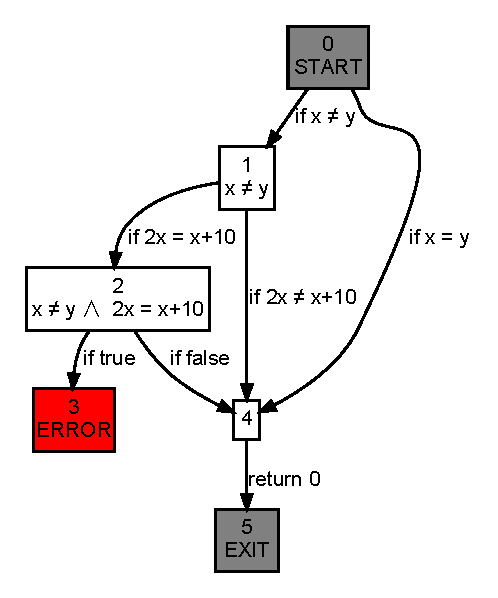
\includegraphics[height=7cm]{figs/exampleAbstraction/exampleAbstraction.eps}
	\caption{Abstraction that models the code in \cref{fig:randomHard}. The condition inside \code{assert false} has been negated and a special \code{ERROR} node has been added. Notice that node 4 cannot limit the values of $x$ nor $y$ since many executions paths with different valuations of the variables join there.}
	\label{fig:randomHardExampleAbstraction}
\end{figure}

A tool could try to construct a precise model of the program, a model that contains a path if and only if that path is possible in the program. Such models tend to capture too many constraints about the program, some of which might not be needed to check a given safety property. Since model checking in general is undecidable we know that such models are often too complex to verify. Instead, verification tools tend to create over-approximate abstractions that are simpler but contains executions that are not possible in the actual program. If it is possible to show that an over-approximate abstraction is error-free, then the program must also be error-free, since the program is contained in the model.

If, however, the model includes a path that leads to an error, it is uncertain if it signals a real error or if the path exists because the model is too coarse. If such paths are reported as errors, some of them can be spurious: verification is complete but usually not sound. Verification tools usually start with a very coarse abstraction and then try to refine it by pruning spurious paths that leads to an error.

The tools \SLAM~\cite{slam2001} and \BLAST~\cite{blast2007} take verification to the next level. They both start with a coarse abstraction of the program. The tools then search for paths leading to errors in their abstract model of the program. If no such paths exist, they are done. However, when a path exists in their abstractions, they check if that path is feasible in the original program by executing the path symbolically and using a constraint solver to validate the constraints generated. If the path is feasible, they have found a true error. If the path is not feasible, then their abstractions are too coarse and they refine their abstractions with new predicates. Such tools are both sound and complete, but unfortunately will not always halt with an answer. Both \SLAM and \BLAST have small sources of unsoundness and incompleteness in them. For example, \BLAST does not model integer overflow, some infeasible paths cannot be proved as such by their decision procedures, and \SLAM uses a logical model of memory where pointer arithmetic is ignored.

\section{Synergy}
\SYNERGY is a predecessor to \DASH and builds on lightweight symbolic execution and testing from \CUTE and verification methods as used in \SLAM and \BLAST. \SYNERGY maintains both an under-approximation like \CUTE but also maintains an over-approximation of the program like \SLAM and \BLAST. The over-approximation is used to guide what tests to execute while the tests guide which refinements of the abstraction are to be made. In a sense the two techniques work together in synergy, thereby the algorithm's name.

The algorithm first finds a path to an error in the over-approximation and then tries to create concrete input to the procedure-under-test such that at least one unexplored step in the path is executed. If \SYNERGY is not able to generate such input, it removes the path from the over-approximation. If \SYNERGY is able to move at least a single step forward, it concretely executes the program and thereby increases the under-approximation. \SYNERGY is able to analyze single-procedure C programs with integer variables and arithmetic.

\section{DASH}
\DASH~\cite{dash2010} builds on the ideas of \SYNERGY~\cite{synergy2006}. \DASH can additionally handle interprocedural programs with pointers and has a more efficient implementation. As in \SYNERGY, \DASH maintains an over- and under-approximation of the program being tested.

There are three possible outcomes of executing \DASH on a program instrumented with a safety property: 1) \DASH never halts and executes forever, 2) \DASH halts and reports that the safety property is violated and 3) \DASH states that the program never violates the safety property. If \DASH reports that the safety property is violated, then \DASH has found a concrete execution the causes a safety property violation. If \DASH reports that the safety property is never violated then the over-approximation is a proof thereof, since the states violating the property are no longer present in the over-approximation. This implies that \DASH is both sound and complete, if it terminates.

Our presentation of the \DASH algorithm is fundamentally different from the original presentation in the \DASH article~\cite{dash2010}. Our presentation tries to remove points of confusion while also adding missing details that are not described properly in the article.

To run \DASH on a program instrumented with a safety property, as was described in \cref{sec:safetyProperties}, one constructs the initial over-approximate abstraction and runs \DASH on it. The abstraction of the program is initially equivalent to the control flow graph of the program where variables are not constrained yet. When given the abstraction, \DASH will perform the same operations as \SYNERGY does. It will first try to find a path in the abstraction that leads to an error. It will check if the path is feasible in the original program at least one step beyond a so-called frontier. If the path is feasible, it will be executed concretely and \DASH will detect if an error was reached during execution. If the path is not feasible, the over-approximation will be refined to remove the infeasible path. If \DASH is not able to find a path to an error in the over-approximation, the program satisfies the safety property.

\DASH as presented by the \DASH article can load test input for concrete executions when starting up, such that the under-approximation can be kick-started. In this presentation this technique has been left out as it only serves as an optimization.

Our presentation of \DASH is broken up into two implementations:
\begin{enumerate}
	\item \DASHint is an implementation that can handle a single procedure which is allowed to take integer arguments, perform integer arithmetic but it is not allowed to call other procedures. \DASHint is essentially equivalent to the \SYNERGY algorithm.
	
	\item \DASHcall is an extension of \DASHint that can also handle calls to other procedures. Only the main procedure may use the \code{error} statement. This limitation can be rectified by using global variables and checking them in the main procedure. See  \cref{sec:dashCall:errorInSubprocedures} for how this could be done.
\end{enumerate}

We describe each of these implementations separately, starting with \DASHint in \cref{ch:dashInt}. \DASHcall is explained in \cref{ch:dashCall}.

%%%%%%%%%%%%%%%%%%%%%%%%%%%%%%%%%%%%%%%%%%%%%%%%%%%%%%%%%%%%%%%%%%%%%%%

\chapter{Analyzing integer programs with DASH$_{int}$}
\label{ch:dashInt}
This chapter presents the \DASHint algorithm, which is able to analyze single procedure integer programs and thus constitutes a subset of the \DASH algorithm.

\DASHint is divided into multiple procedures that together implement the \DASHint algorithm. The main procedure of \DASHint is \classname{DashLoop}. It calls other procedures which in turn may again call other procedures. \cref{fig:dashInt:procedureOverview} shows the call hierarchy for each procedure of the \DASHint algorithm and in which section the procedure is described.

\begin{figure}

\newcommand{\procedureAt}[2]{\classname{#1}\\{\small#2}}

\begin{spacing}{0.8}
\begin{tikzpicture}[%
	->,
	shorten >=2pt,
	>=stealth,
	node distance=0.91cm,
	pil/.style={
	->,
	thick,
	shorten =2pt,}
]

\node [align=left]												       (loop)   {\procedureAt{DashLoop}{\cref{sec:dashInt:mainLoop}}};
\node [align=left, above right=2cm and 1cm of loop] 	    	       (path)   {\procedureAt{FindAbstractErrorPath}{\cref{sec:dashInt:findabstracterrorparth}}};
\node [align=left, right=of loop, below=of path.west,anchor=west]      (trace)  {\procedureAt{ConvertToRegionTraceWithAbstractFrontier}{\cref{sec:dashInt:convertToRegionTrace}}};
\node [align=left, right=of loop, below=of trace.west,anchor=west]     (extend) {\procedureAt{ExtendFrontier}{\cref{sec:dashInt:extendFrontier}}};
 \node [align=left, above right=-0.4cm and 1.5cm of extend,anchor=west](symb)   {\procedureAt{ExecuteSymbolic}{\cref{sec:dashInt:executeSymbolic}}};
 \node [align=left, right=of extend, below=of symb.west,anchor=west]   (sat)    {\procedureAt{IsSAT}{\cref{sec:dashInt:isSat}}};
 \node [align=left, right=of extend, below=of sat.west,anchor=west]    (pred)   {\procedureAt{RefinePred}{\cref{sec:dashInt:refinePred}}};
  \node [align=left, right=of pred,anchor=west]                        (wp)     {\procedureAt{WP}{\cref{sec:dashInt:wp}}};


\node [align=left, right=of loop, below=of extend.west,anchor=west](test) {\procedureAt{RunTest}{\cref{sec:dashInt:runtest}}};
\node [align=left, right=of loop, below=of test.west,anchor=west]  (error) {\procedureAt{IsErrorRegionReached}{\cref{sec:dashInt:iserrorregionreached}}};
\node [align=left, right=of loop, below=of error.west,anchor=west] (refine) {\procedureAt{RefineGraph}{\cref{sec:dashInt:refinegraph}}};



\draw[->] (loop.east) --(path.west);
\draw[->] (loop.east) --(trace.west);
\draw[->] (loop.east) --(extend.west);
 \draw[->] (extend.east) --(symb.west);
 \draw[->] (extend.east) --(sat.west);
 \draw[->] (extend.east) --(pred.west);
  \draw[->] (pred.east) --(wp.west);
\draw[->] (loop.east) --(test.west);
\draw[->] (loop.east) --(error.west);
\draw[->] (loop.east) --(refine.west);
\end{tikzpicture}
\end{spacing}
\caption
{
	Overview over called procedures in \DASHint. The procedures are listed in call order. For example \classname{DashLoop} calls \classname{ExtendFrontier} before \classname{RunTest}.
}
\label{fig:dashInt:procedureOverview}
\end{figure}

The next sections describe what types of programs \DASHint handles and the key region graph data structure. Afterwards the algorithm itself is presented starting with the \classname{DashLoop} procedure. Then all sub procedures of \classname{DashLoop} are described, excluding \classname{ExtendFrontier} and its sub procedures, which has been given their own sections because of their importance. After all of the procedures used by \DASHint have been explained, we perform a complete walk through of how \DASHint analyzes the example procedure \code{abs} introduced in \cref{ch:dashBackground}. Finally, we describe key problems encountered and changes we have made to implement \DASHint in \cref{sec:dashInt:challenges}.

\section{Program structures supported by DASH$_{int}$}
This section describes in detail what types of programs \DASHint analyzes and what are assumed about them.

\DASHint analyzes programs instrumented with \code{error} statements that are executed whenever a desired safety property has been violated. Thus the safety property itself is never passed to \DASHint and the objective is instead to ensure that no \code{error} statements are reachable. This type of program transformation was presented in \cref{ch:dashBackground}, \cref{fig:openCloseExample}.

The program $\mathpzc{P}$ is restrained to a single procedure where the following statements are allowed:
\begin{itemize}
	\item Assignments of the form \code{v := e} where \code{v} is a local variable and \code{e} is an expression.
	
	\item Conditionals of the form \code{if c goto l} where \code{c} is a conditional expression and \code{l} is a program location.
	
	\item An \code{error} statement.
\end{itemize}

The \code{return} statement is allowed but seen as no-operation statement. Expressions and conditionals are restricted to simple forms and a grammar is given in \cref{fig:dashInt:grammar}. The expressions and conditionals are constrained, such that they are side effect free and cannot be nested.

\begin{figure}
\centering
\setlength{\grammarindent}{6.5em}
\begin{grammar}
<expr> ::= <operand>
   \alt '-' <operand>
   \alt <operand> <binop> <operand>

<binop> ::= '+'
          | '-'
          | '*'
          | '/'
          | '\%'
          | '\textasciitilde'
          | '\^{}'
          | '|'
          | '\&'
          | '$\ll$'
          | '$\gg$'
          | '$\ggg$'

<cond> ::= '\code{true}'
      \alt '\code{false}'
      \alt <operand> <cond-op> <operand>


<cond-op> ::= '=='
         | '$\neq$'
         | '\textless'
         | '\textgreater'
         | '$\leq$'
         | '$\geq$'

<operand> ::= <identifier>
          \alt <constant>
\end{grammar}
\caption
{
	Grammar showing the allowed forms for expressions and conditionals.
}
\label{fig:dashInt:grammar}
\end{figure}
Nested expression or expressions with side effects can be rewritten to simple expressions by introducing new temporary variables. The \code{while} and \code{for} loop constructs can be desugared into \code{if c goto l} and \code{goto l} statements. Simple \code{goto l} statements can be modeled using \code{if true goto l}.

The example procedure \code{abs} from \cref{fig:abs}, here reproduced as \cref{fig:dashInt:exampleProgram}, functions as a running example program for explaining \DASHint. Notice that the program is not written in a form that \DASH can analyze. Translating it to a version that can be analyzed is straightforward since the \code{if} statement can easily be converted to an \code{if c  goto l} statement and the \code{assert} statement is analogues to an \code{if} with an \code{error} statement inside. The raw desugared version, which can be analyzed by \DASH, is shown in \cref{fig:dashInt:exampleProgramDesugared}.

\begin{figure}
\newsavebox{\dashIntAbsProgramSugared}
\begin{lrbox}{\dashIntAbsProgramSugared}
\begin{lstlisting}[showlines=true,mathescape]
int abs(int a)
{
	if(a < 0)
		a = -a;
	assert a $\geq$ 0;
	return a;
}





\end{lstlisting}
\end{lrbox}

\newsavebox{\dashIntAbsProgramDesugared}
\begin{lrbox}{\dashIntAbsProgramDesugared}
\begin{lstlisting}[mathescape]
int abs(int a)
{
	if a $\geq$ 0 goto l1;
	a = -a;

 l1:
	if a $\geq$ 0 goto l2;
	error;

 l2:
	return a;
}
\end{lstlisting}
\end{lrbox}
\centering
\subfloat[\DASHint example procedure \code{abs}.]
{
	\usebox{\dashIntAbsProgramSugared}
	\label{fig:dashInt:exampleProgram}
}
\hfil
\subfloat[Desugared version of \code{abs}.]
{
	\usebox{\dashIntAbsProgramDesugared}
	\label{fig:dashInt:exampleProgramDesugared}
}
\caption
{
	\protect\subref{fig:dashInt:exampleProgram} shows the \code{abs} procedure  in a non-desugared version. \protect\subref{fig:dashInt:exampleProgramDesugared} shows the same procedure but desugared into a form that \DASHint accepts.
}
\end{figure}

\section{Region Graph}
\label{sec:dashInt:regionGraph}
A \textit{region graph} is the central data structure used by \DASH. It models both the over-approximation and under-approximation of the reachable state space. A region graph is essentially the same as the example abstraction mentioned in \cref{sec:verification} used by verification tools, but with the added feature that it also contains concrete executions that represent the under-approximation. In the \DASH paper the under-approximation is contained in a separate data structure called a \textit{forest}. We chose to embed the states from the forest directly into the region graph, due to frequent lookup of which states that are contained in a region.

A region graph is a set of nodes and edges. Nodes are called regions and model a set of states that satisfy the predicate that is attached to the region. Edges between nodes are labeled with the program statements. Initially the region graph is equivalent to the control flow graph for the program. The first region is called the \textit{initial region}, which is the region that exists before any statements have been executed. If a region has an outgoing edge labeled with an \code{error} statement, the region is termed an \textit{error region}. Our regions keep the edges with an \code{error} statement, but these could have been removed and concrete execution would have to halt if an error region was reached.

When creating a region graph, \code{if c goto l} statements become two edges with assumes, one with \code{assume c} and the other with \lstinline[mathescape]{assume $\neg$c}. When presenting the graphs, the following conventions apply:

\newcommand{\graphcolor}[2]{\textbf{\textcolor[HTML]{#1}{#2}}}

\begin{itemize}
	\item Regions are displayed as boxes, and edges between them correspond to potential program state transitions. Regions initially have a unique identification number assigned but it is only used for presenting the graphs. Edge labels correspond to statements in the program.
	
	\item For \code{assume c} statements, only the condition \code{c} is written as edge labels to preserve space. To distinguish them from other edge labels, the condition \code{c} is written with a \graphcolor{0000FF}{blue} font.
	
	\item The initial region is colored \graphcolor{808080}{gray}. The special error regions, the regions before an \code{error} statement, are colored \graphcolor{FF0000}{red}. Regions and edges that cannot be reached from the initial region are colored \graphcolor{FFD700}{yellow}. Unreachable error regions are colored \graphcolor{F75D59}{light red}.
	
	\item A region models all states that satisfies the attached predicate. An example predicate could be $a > 0$. Predicates are shown below the region identification number. If the region predicate is \code{true}, which is trivially satisfied by all states, it is omitted for brevity.
	
	\item Regions can have concrete states attached to them originating from a concrete execution of the procedure. The list of states are shown in curly braces \{\dots\}, with individual states in square brackets [\ldots]. They constitute the under-approximation maintained by \DASH. A number $\#n$ represents how many statements have been executed before reaching the state. An example state could be $\#3[a\mapsto0]$. Without $\#n$ it can be hard to distinguish states inside a loop from each other.
\end{itemize}

\cref{fig:dashInt:regionGraph:initial} shows the initial region graph for the \code{abs} procedure presented in \cref{fig:dashInt:exampleProgram}. Notice that the region graph is identical to the control flow graph of the program.

\Cref{fig:dashInt:regionGraph:traceIncluded} shows the region graph after a test has been executed and the concrete states have been added to the region graph. It can be seen that \code{abs} was called with $a \mapsto 0$. It can also be seen that the error region has not been reached by the test, since the error region contains no states. The concrete states of a particular concrete execution are linked together as a doubly-linked list. It is therefore possible to find both the parent and child state of a particular state.

\begin{figure}
	\centering
	\subfloat[Initial graph]
	{
		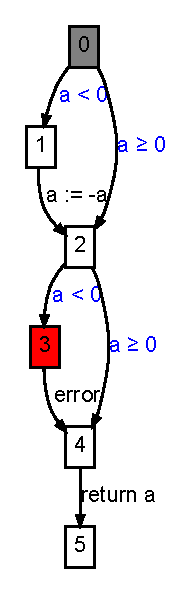
\includegraphics[height=7cm]{{figs/subtleAbsOverflowFail/2test.graph.0.init}.eps}
		\label{fig:dashInt:regionGraph:initial}
	}
	\hfil
	\subfloat[States added]
	{
		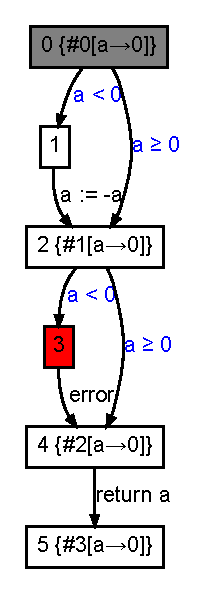
\includegraphics[height=7cm]{{figs/subtleAbsOverflowFail/5test.graph.0}.eps}
		\label{fig:dashInt:regionGraph:traceIncluded}
	}
	\hfil
	\subfloat[With predicates, splitting region 2]
	{
		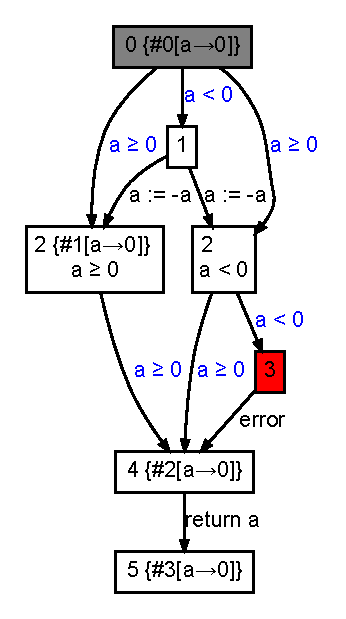
\includegraphics[height=7cm]{{figs/subtleAbsOverflowFail/8test.graph.1}.eps}
		\label{fig:dashInt:regionGraph:withPredicates}
	}
	\caption
	{
		\protect\subref{fig:dashInt:regionGraph:initial} shows the initial region graph for the \code{abs} procedure seen in \cref{fig:dashInt:exampleProgram}. \protect\subref{fig:dashInt:regionGraph:traceIncluded} shows how states from a concrete execution are added to the region graph. It can be seen that \code{abs} was called with $a \mapsto 0$. \protect\subref{fig:dashInt:regionGraph:withPredicates} shows how equivalence classes of states are modeled in the graph, here by splitting region 2.
	}
\end{figure}

Formally, let $\Sigma$ be the state space for a procedure $P$. It contains all the different valuations of the variables known by $P$. Program state can be altered when statements are executed which naturally defines a function $\to: \Sigma \to \Sigma$ from one state to another for $P$.

The region graph models equivalence classes of states $\Sigma_\simeq$, such that states in an equivalence class are thought to have the same properties. An example could be that all states with $x > 0$ are modeled to be in the same equivalence class. \Cref{fig:dashInt:regionGraph:withPredicates} shows how such equivalence classes can be expressed in the region graph. Region $2$ has been split into two. One with the predicate $a < 0$ and the other with the negation $a \geq 0$. The region with the predicate $a \geq 0$ cannot enter the error region $3$, since an edge has been removed. The edge would have been labeled with an \code{assume} $a < 0$ statement, which cannot be satisfied under the condition $a \geq 0$.

Edges in the region graph correspond to possible state changes between equivalence classes and we denote the edges $\to_\simeq: \Sigma_\simeq \times \Sigma_\simeq$.

When \DASH begins execution, the region graph is equivalent to the control flow graph of the program and all regions contain the single predicate \code{true}, which allows any variable to take any value. Whenever the \DASH algorithm refines the abstraction, a region is split into two using a predicate that is suitable for refinement. The main algorithm, including refinement, will be explained in the following sections. 

\section{The main loop}
\label{sec:dashInt:mainLoop}
\classname{DashLoop} is the main loop of \DASHint and pseudocode is provided in \cref{alg:dashInt:dashloop}. It takes a procedure $P$ and a region graph $G$ as input and will return \pass or \fail depending on whether an error region is reachable. If it reports a failure, it will also return the input values needed to reach the error region. In case the program passes, the refined region graph will be returned as proof of the error region being unreachable.

\begin{thesisalgorithm}
\caption{\classname{DashLoop}$(P, G = \langle \Sigma_\simeq, \rightarrow_\simeq \rangle)$}
\label{alg:dashInt:dashloop}
Returns:\\
(\fail, $t$), where $t$ is a list of input values for reaching error; or\\
(\pass, $G$), where $G$ is a proof that the error cannot be reached.\\

\begin{algorithmic}[1]
	\Loop		
		\State $\tau := \classname{FindAbstractErrorPath}(G)$
		\If{$\tau=\nopath$}
			\State \Return $(\pass, G)$
		\EndIf\\
		
		\State $\tau_c := \classname{ConvertToRegionTraceWithAbstractFrontier}(\tau, G)$
		\State $\langle t, \rho \rangle := \classname{ExtendFrontier}(\tau_c, P)$
		\If{$t \neq \unsat$}
			\State $G := \classname{RunTest}(t, P, G)$
			\If{$\classname{IsErrorRegionReached}(G)$}
				\State \Return $(\fail, t)$
			\EndIf
		\Else
			\State $G := \classname{RefineGraph}(\rho, \tau_c, G)$
		\EndIf
	\EndLoop
\end{algorithmic}
\end{thesisalgorithm}

\classname{DashLoop} starts by calling \classname{FindAbstractErrorPath} to find an abstract error path $\tau$ in the region graph $G$ that leads to an error region. Whenever we refer to a \textit{path} or write $\tau$ it is the abstract error path returned by \classname{FindAbstractErrorPath} we are referring to. If \classname{FindAbstractErrorPath} is unable to find a path that leads to an error region, then the graph $G$ proves that no error state is reachable in $P$ since $G$ is an over-approximation of $P$. If a path is found, then \classname{ConvertToRegionTraceWithAbstractFrontier} finds the last region in the abstract error path $\tau$ with a concrete state. This region is denoted $S_{k-1}$. The state found in $S_{k-1}$ is followed back to the initial region and this leads to the trace $\langle S_0, \ldots, S_{k-1} \rangle$ that constitutes the first part returned by \classname{ConvertToRegionTraceWithAbstractFrontier}. The last part of the trace is the region in $\tau$ right after $S_{k-1}$ which we denote $S_k$. The edge between $S_{k-1}$ and $S_k$ is termed the \textit{frontier}. The new trace $\tau_c= \langle S_0, \ldots, S_{k-1}, S_k \rangle$, returned by \classname{ConvertToRegionTraceWithAbstractFrontier}, is created in this way such that the trace leading up to the frontier is known to be feasible. If the trace is found infeasible, it must be because of the frontier edge. Whenever we refer to a \textit{trace} or use the symbol $\tau_c$, then we are referring to the trace returned by \classname{ConvertToRegionTraceWithAbstractFrontier}.

The next step is to attempt to extend the frontier by finding a test input that will cross the frontier edge when executed concretely. This will bring us at least one step closer to the error region and to showing that the error region is reachable. The \classname{ExtendFrontier} procedure attempts to find such test input, but if such a test does not exist, it finds a predicate that can be used to refine the region graph, such that the current trace $\tau_c$ is eliminated from $G$. If \classname{ExtendFrontier} finds a test input, then it will return the pair $\langle t, \text{\code{true}} \rangle$, where $t$ is the input values that will push execution over the frontier edge. \classname{RunTest} is used to execute the test on an instrumented version of $P$, where for each executed statement the concrete state of the variables is saved in the reached region. An updated region graph is returned from \classname{RunTest}, with the new concrete states added.

If an error region is reached during concrete execution, then \classname{RunTest} has added a state to it. The procedure \classname{IsErrorRegionReached} returns \code{true} if there is an error region that contains a concrete state. If \classname{IsErrorRegionReached} returns \code{true} then the input values $t$ must be the input that led to the error being reached. This is evident since the error regions are checked after each \classname{RunTest} invocation, and thus before \classname{RunTest} was called with $t$, the error regions did not contain any states. Therefore the concrete state must have arisen because of the latest \classname{RunTest} invocation with $t$ as input. 

Even if the test did not reach the error region sought by the path $\tau$, the frontier has been advanced and concrete states will have come closer to the error region. Given that \classname{FindAbstractErrorPath} uses a deterministic graph search algorithm, which is not a requirement, the same abstract path will be found in the next iteration of \classname{DashLoop}. However \classname{ConvertToRegionTraceWithAbstractFrontier} will find a longer trace where the frontier has been pushed forward. Remember that the last test crossed the last frontier, and therefore a state was added to region $S_k$. This pushes the next frontier found by \classname{ConvertToRegionTraceWithAbstractFrontier} forward by at least one region and in this way progress is achieved.

If \classname{ExtendFrontier} is not able to find a test input, then it returns a suitable refinement predicate $\rho$. The definition of a suitable refinement predicate is provided in \cref{sec:dashInt:refinePred}, but the basic property is that it excludes the current trace $\tau_c$ and if the predicate is not satisfied at region $S_{k-1}$ then region $S_k$ cannot be reached. \classname{RefineGraph} refines the region graph by using these properties of the refinement predicate. Specifically it splits region $S_{k-1}$ into two. One which has the refinement predicate $\rho$ added and one with the negation $\neg\rho$ added. Because of the properties that $\rho$ has, the region with $\neg\rho$ added cannot reach $S_k$ and therefore the edge to $S_k$ is removed. The refinement process of splitting region $S_{k-1}$ into two can be seen in \cref{fig:dashInt:refineRegion} and is also explained in greater detail in \cref{sec:dashInt:refinePred}.

\begin{figure}
\def \scale {0.65}
	\centering
	$\vcenterimage{figs/refineRegion/before.eps}{\scale}
	\vcenterarrow
	\vcenterimage{figs/refineRegion/after.eps}{\scale}$
	\caption
	{
		Refinement process of region $S_{k-1}$, which contains the region predicate $\rho_{k-1}$, using the refinement predicate $\rho$. Notice that the region with $\neg\rho$ added has the edge to region $S_k$ removed.
	}
	\label{fig:dashInt:refineRegion}
\end{figure}

The resulting graph is a better approximation of the program. The graph reflects that to follow the edge $(S_{k-1}, S_k)$ then $\rho$ must be satisfied. \classname{DashLoop} starts the next iteration and tries to find a new abstract error path to the error region, since the current one has now been eliminated.

\classname{DashLoop} has now been described. We now begin to describe the procedures that \classname{DashLoop} calls, starting with \classname{FindAbstractErrorPath}.

\subsection{\classname{FindAbstractErrorPath}}
\label{sec:dashInt:findabstracterrorparth}
The goal of \classname{FindAbstractErrorPath} is to find a path in the region graph $G$ from the initial region to an error region. If the error regions are unreachable, then the special value \nopath is returned. The \DASH article does not describe how the path should be found. It could be implemented using a standard breadth-first search from the initial region, stopping when an error region is encountered. 

One could also use a depth-first search, and this should not make a difference to how \DASH works. However, for a developer, it is most beneficial to describe the shortest path leading to an error, instead of a longer one involving irrelevant operations.

\Cref{fig:dashInt:pathExample:regionGraph} shows the region graph for the \code{abs} procedure after an initial test has been executed, without reaching the error region. The path $\langle 0, 2, 3 \rangle$ is shown in \Cref{fig:dashInt:pathExample:abstractpath} using dashed red edges (\graphcolor{FF0000}{- - -}). It is the shortest abstract error path found by \classname{FindAbstractErrorPath} using a breadth-first algorithm. By convention, whenever we present a path in a region graph, the path is always shown using dashed red edges.

The path is converted by \classname{ConvertToRegionTraceWithAbstractFrontier} to a trace that follows a concrete execution. We describe \classname{ConvertToRegionTraceWithAbstractFrontier} in the next section.

\begin{figure}
\def \height {6.3cm}
	\centering
	\begingroup
	\captionsetup[subfigure]{width=3cm}
	\subfloat[Region graph]
	{
		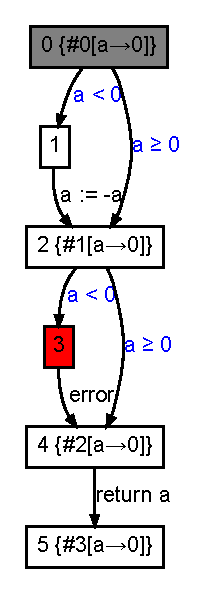
\includegraphics[height=\height]{{figs/subtleAbsOverflowFail/5test.graph.0}.eps}
		\label{fig:dashInt:pathExample:regionGraph}
	}
	\hfil
	\subfloat[Abstract error path $\langle 0, 2, 3 \rangle$]
	{
		\includegraphics[height=\height]{{figs/subtleAbsOverflowFail/6test.graph.1.path}.eps}
		\label{fig:dashInt:pathExample:abstractpath}
	}
	\hfil
	\subfloat[Concrete error trace with frontier]
	{
		\includegraphics[height=\height]{{figs/subtleAbsOverflowFail/7test.graph.1.trace}.eps}
		\label{fig:dashInt:pathExample:concfrontier}
	}
	\endgroup
	\caption
	{
		\protect\subref{fig:dashInt:pathExample:regionGraph} shows the region graph for the \code{abs} procedure in \cref{fig:dashInt:exampleProgram} where \code{abs} has been called with the concrete input $a \mapsto 0$ and concrete states have been added to the graph.
		\protect\subref{fig:dashInt:pathExample:abstractpath} shows the abstract error path with dashed red lines found by \classname{FindAbstractErrorPath}.
		\protect\subref{fig:dashInt:pathExample:concfrontier} shows the path converted to a trace. The part that follows a concrete execution is shown with green edges while the frontier edge is shown in red.
	}
	\label{fig:dashInt:pathExample}
\end{figure}

\subsection{\classname{ConvertToRegionTraceWithAbstractFrontier}}
\label{sec:dashInt:convertToRegionTrace}
\classname{ConvertToRegionTraceWithAbstractFrontier} is responsible for converting an abstract error path $\tau$ into a trace that follows a concrete execution for as long as possible, and then takes one extra step in the direction of the abstract error path. This is completed by finding the last region in $\tau$ that contains a state, which we name $S_{k-1}$ for the region and $s_{k-1}$ for the particular state. If the region contains multiple states, then the newest one is chosen. The reason for picking the newest state is described in \cref{sec:dashInt:challenges:whichStateToPick}.

The parent relationship of $s_{k-1}$ is used to search backwards to the initial region and the execution trace $\langle s_0, \ldots, s_{k-1} \rangle$ is obtained. It is assumed that one can find the regions which the states are attached to, such that the trace $\langle S_0, \ldots, S_{k-1} \rangle$ of regions can be obtained. This is the part of the trace that follows a concrete execution. Notice that $\langle S_0, \ldots, S_{k-1} \rangle$ might not follow the path taken by $\tau$, which we describe in \cref{sec:dashInt:challenges:mustTraceFollowPath}. Next the frontier edge is added, by adding region $S_k$, which is the region located after region $S_{k-1}$ in the abstract path. The trace $\tau_c = \langle S_0, \ldots, S_{k-1}, S_k \rangle$ is returned. The frontier is unexplored in the sense that no concrete test have ever crossed that particular edge in the abstraction.

\cref{fig:dashInt:pathExample:concfrontier} shows the trace $\tau_c=\langle0,2,3\rangle$ found when the path shown in \cref{fig:dashInt:pathExample:abstractpath} is converted. The part of the trace $\langle S_0, \ldots, S_{k-1} \rangle$ that follows a concrete execution is shown using \graphcolor{00FF00}{green} edges while the frontier $(S_{k-1}, S_k)$ is shown in \graphcolor{FF0000}{red}. The path $\tau$, from which $\tau_c$ is created, is nearly always longer than $\tau_c$. The only case where they have the same length, is when $S_k$ is an error region and $S_{k-1}$ already contains a state from a concrete execution. In the cases where the path is longer than the trace, the remaining part of the path, the part from region $S_k$ to the error region, is shown using red dashed edges (\graphcolor{FF0000}{- - -}) to aid the reader in where the path $\tau$ sought to reach. Thus, the reader should remember that when a trace $\tau_c$ is depicted in a figure, then the dashed lines are \textit{not} part of the trace.

The reason that \DASH converts an abstract error path into a region trace with a frontier is because then it is known that the part of the trace that follows a concrete execution is feasible. Thus \DASH knows that region $S_{k-1}$ is reachable. If \DASH finds that the whole trace is infeasible, then \DASH knows that it is the frontier edge that made it infeasible. Then the frontier is refined by \classname{RefineGraph}, as explained later in \cref{sec:dashInt:refinegraph}, such that the trace $\tau_c$ is excluded from the region graph and the abstraction is made more precise.

The first time an abstract error path $\tau$ is converted to a trace $\tau_c$ there are no regions in $G$ that has been reached by concrete execution. For this case \classname{ConvertToRegionTraceWithAbstractFrontier} assumes that there is a concrete state in the initial region, even though there is not. The trace $\tau_c$ does then only contain the frontier edge, which is the first edge contained in the path $\tau$. This assumption is not problematic since all test executions start in the initial region and therefore trivially reaches it.

\subsection{\classname{RunTest}}
\label{sec:dashInt:runtest}
\classname{RunTest} is responsible for executing a procedure P concretely and record the concrete states for each executed statement. \classname{RunTest} is given a list of input values $t$, the procedure $P$ and the graph $G$. It runs a concrete test on $P$ with $t$ as input. During execution the state of the variables is recorded and added to the graph $G$. The concrete states are later used to check if the test reached an error region and to compute traces as described in \cref{sec:dashInt:convertToRegionTrace}.

The states can be recorded by executing an instrumented version of $P$ and recording concrete values of variables at each program point. Alternatively one could simulate the code and then record the state at each step in the simulator.

Common for both solutions are that they need to follow the concrete execution in the region graph to insert the states in the correct regions. For example, if execution is at a region which has multiple outgoing edges, \classname{RunTest} needs to figure out what edge the current concrete execution takes. Since the equivalence classes modeled are disjoint there is only a single edge that can be traversed. To check if an \code{assume c} edge is traversable, the conjunction of the region predicate and the condition \code{c} has to evaluate to \code{true} by inserting the concrete values of all variables into them. For assignment edges the state needs to be updated first and then the region predicates can be evaluated, to find the single one that evaluates to \code{true}.

The implementation of \DASH in \YOGI used a simulator to both concretely execute tests and to perform symbolic execution, whereas our \Java implementation uses an instrumented version to execute the test~\cite{dash2010}. We describe our \classname{RunTest} implementation in \cref{sec:dashImpl:runtest}.

\subsection{\classname{IsErrorRegionReached}}
\label{sec:dashInt:iserrorregionreached}
\classname{IsErrorRegionReached}  is responsible for checking if an error region has been reached. \classname{IsErrorRegionReached} takes as input the region graph $G$. It then runs through all regions and checks if a concrete state has been added to an error region, in which case the error region has been reached. If a state is found in an error region then the procedure returns \code{true}, otherwise it returns \code{false}. The pseudocode for \classname{IsErrorRegionReached} is shown in \cref{alg:dashInt:isErrorRegionReached}. Notice that the syntax \textbf{let} $\langle \_, states \rangle = S$ is used to unpack region $S$ into its region predicate and its contained states. However, an underscore \_ is used to denote that the region predicate is unused for this particular procedure.

\begin{thesisalgorithm}
\caption{\classname{IsErrorRegionReached}($G = \langle \Sigma_\simeq, \rightarrow_\simeq \rangle$)}
\label{alg:dashInt:isErrorRegionReached}
Returns:\\
\code{true}, if a test has reached an error region; or\\
\code{false}, if no test has.\\

\begin{algorithmic}[1]
	\For{$S \in \Sigma_\simeq$}
		\State \Let $\langle \_, states \rangle = S$
		\If{$\classname{IsErrorRegion}(S) \wedge states \neq \emptyset$}
			\State \Return \code{true}
		\EndIf
	\EndFor
	\State \Return \code{false}
\end{algorithmic}
\end{thesisalgorithm}

To prevent an expensive search through all regions an actual implementation should maintain a set of error regions and only loop through that particular set to check if one of them contains a newly added state. Another solution could be to let \classname{RunTest} report if an error region was reached during execution. \classname{RunTest} could do this be setting a flag if it adds a state to an error region.

\subsection{\classname{RefineGraph}}
\label{sec:dashInt:refinegraph}
\classname{RefineGraph} is responsible for altering the region graph such that a trace $\tau_c$ that was found infeasible, i.e. test input could not be generated for it, is removed from the graph and therefore from the over-approximation. A suitable refinement predicate is used to refine the region graph. How the suitable refinement predicate is obtained is described in \cref{sec:dashInt:refinePred}.

\classname{RefineGraph} takes as input an infeasible trace $\tau_c$, a suitable refinement predicate $\rho$ and the region graph $G$ to refine. The pseudocode for \classname{RefineGraph} is given in \cref{alg:dashInt:refinegraph}.

\begin{thesisalgorithm}
\caption{\classname{RefineGraph}($\rho, \tau_c = \langle S_0, \ldots, S_{k-1}, S_k \rangle, G = \langle \Sigma_\simeq, \rightarrow_\simeq \rangle$)}
\label{alg:dashInt:refinegraph}
Returns: $\langle \Sigma_\simeq, \rightarrow_\simeq \rangle$, the refined region graph.
\begin{algorithmic}[1]
	\State \Let $\langle \rho_{k-1}, states \rangle = S_{k-1}$
	\\
	
	\If{$k = 1$} \Comment{Initial region refinement}
		\State \Return $\langle \Sigma_\simeq, \rightarrow_\simeq \setminus {(S_0, S_1)} \rangle$
	\EndIf
	
	\\
	
	\State $\Sigma_\simeq^* := \Sigma_\simeq \setminus \{S_{k-1}\}$ \Comment{Remove $S_{k-1}$}
	\State $\rightarrow_\simeq^* := \rightarrow_\simeq \setminus \{(S, S_{k-1}) \mid S \in \classname{Parents}(S_{k-1}) \}$
	\State $\rightarrow_\simeq^* := \rightarrow_\simeq^* \setminus \{(S_{k-1}, S) \mid S \in \classname{Children}(S_{k-1})\}$	
	\\	
	
	\State $\rho_{k-1}^* := \classname{Simplify}(\rho_{k-1} \wedge \neg \rho)$
	\State $S_{k-1}^* := \langle \rho_{k-1}^*, states \rangle$
	\State $\Sigma_\simeq^* := \Sigma_\simeq^* \cup \{S_{k-1}^*\}$  \Comment{Insert $S_{k-1}^*$}
	\State $\rightarrow_\simeq^* := \rightarrow_\simeq^* \cup \{(S, S_{k-1}^*) \mid S \in \classname{Parents}(S_{k-1})\}$	
	\State $\rightarrow_\simeq^* := \rightarrow_\simeq^* \cup \{(S_{k-1}^*, S) \mid S \in \classname{Children}(S_{k-1})\}$	
	\\	
	
	\State $\rho_{k-1}^{**} := \classname{Simplify}(\rho_{k-1} \wedge \rho)$
	\State $S_{k-1}^{**} := \langle \rho_{k-1}^{**}, \emptyset \rangle$
	\State $\Sigma_\simeq^*$ := $\Sigma_\simeq^* \cup \{ S_{k-1}^{**}\}$
	\State $\rightarrow_\simeq^* := \rightarrow_\simeq^* \cup 	\{(S_{k-1}^{**}, S) \mid S \in \classname{Children}(S_{k-1})\}$
	\If{$\classname{IsSAT}(\rho_{k-1}^{**}) \neq \unsat$} \Comment{Add incoming edges if $\rho_{k-1}^{**}$ is satisfiable}
		\State $\rightarrow_\simeq^* := \rightarrow_\simeq^* \cup \{(S, S_{k-1}^{**}) \mid S \in \classname{Parents}(S_{k-1})\}$
	\EndIf
	
	\\
	
	\State $\rightarrow_\simeq^* := \rightarrow_\simeq^* \setminus \{(S_{k-1}^*, S_k)\}$ \Comment{Remove frontier edge from $S_{k-1}^*$}
	\State \Return $\langle \Sigma_\simeq^*, \rightarrow_\simeq^* \rangle$
\end{algorithmic}
\end{thesisalgorithm}

Lines 3-5 handle the special case of refining the initial region. We first describe the general refinement idea and will come back to this special case afterwards.

The general idea is to split the region before the frontier edge, such that the equivalence class modeled by that region is split into two: one class that will not enter the region after the frontier and one class that might enter it. This is completed by using the given suitable refinement predicate $\rho$. \classname{RefineGraph} creates two new regions that contain the same predicate as the original, but where one region has $\rho$ added and one has $\neg\rho$ added. Thus the equivalence class is split into two. The frontier edge is removed from the region that has $\neg\rho$ added as that edge is now impossible to follow, because of the properties of $\rho$.

More formally, a refinement at the frontier edge $(S_{k-1}, S_k)$ is completed by splitting region $S_{k-1}$ into two. Let $\rho_{k-1}$ be the region predicate of $S_{k-1}$ and let $states$ be the concrete states attached to the region. We can then write region $S_{k-1}$ as $S_{k-1}=\langle\rho_{k-1}, states \rangle$. When region $S_{k-1}$ is split, two new regions are created: $S_{k-1}^*=\langle \rho_{k-1} \wedge \neg \rho, states \rangle$ and $S_{k-1}^{**}=\langle \rho_{k-1} \wedge \rho, \emptyset \rangle$. Notice that region $S_{k-1}^*$, which has $\neg\rho$ added as a predicate, contains all the concrete states that was attached to region $S_{k-1}$. The reason for this is that \classname{RefinePred}, as described in \cref{sec:dashInt:refinePred}, computes a refinement predicate that moves all the concrete states to $S_{k-1}^*$. The two new regions replace the region $S_{k-1}$ that was split. The refinement process was depicted in \cref{fig:dashInt:refineRegion}, when \classname{DashLoop} was described.

Lines 7-9 in the pseudocode remove the split region $S_{k-1}$ from the region graph. Lines 11-15 create and insert region $S_{k-1}^*$. Lines 17-23 insert region $S_{k-1}^{**}$. As can be seen in lines 11 and 17, the predicates attached to the new regions are simplified. We elaborate on how these predicates are simplified in \cref{sec:dashInt:challenges:refineGraph:usatRegions}. Simplification is optional but can be used to keep the predicates concise.

In some cases there are no states that can satisfy the predicate $\rho_{k-1} \wedge \rho$ added to region $S_{k-1}^{**}$. Thus the equivalence class that is modeled is empty. In other words the predicate $\rho_{k-1} \wedge \rho$ is unsatisfiable and thus equivalent to \code{false}. This is detected in line 21 with a call to \classname{IsSAT}, which returns \unsat if the predicate is unsatisfiable. For this case we add the region to the graph but refrain from adding incoming edges. The region is thus carved out of the graph and becomes unreachable. Had we added the incoming edges then \classname{FindAbstractErrorPath} would be able to find a path through the region. Without this check some programs are refined infinitely, as we describe in \cref{sec:dashInt:challenges:refineGraph:usatRegions}. We could have removed the region altogether, however, we keep it as it makes it easier to interpret a series of graphs when regions are not disappearing.

\subsubsection{Refinement of the initial region}
\label{sec:dashInt:refinegraph:initialRegion}
We have had troubles with how \DASH, as described in the \DASH article, handles refinements of the initial region. We elaborate on this in \cref{sec:dashInt:challenges:initialRegion}.

When \classname{RefineGraph} refines an outgoing edge from the initial region, the edge is removed without splitting the initial region. This is completed in lines 3-5 in the \classname{RefineGraph} pseudocode.

In general, if there exists only one path that can reach an edge, and have it as the frontier, then if the path is found infeasible, the edge can be removed altogether. Since no other paths can lead to it, no harm has been made by removing it. If another path could lead down to the edge, then that path may lead to a different state that could allow the edge to be traversed. We require that only one path leads to the initial region, and then removing the edge when refining the initial region is a valid refinement.

There are cases where the initial region may be reached by more than one trace. For example, when the initial region is part of a loop, a trace could reach the initial region by taking $x$ iterations of the loop. Thus more than one trace lead to the initial region. For such cases we could hoist the initial region by constructing a dummy initial region above with an \code{assume true} edge leading to the original initial region.

\subsubsection{Refinement example}
\cref{fig:dashInt:refinegraph} provides an example of refinement.  \cref{fig:dashInt:refinegraph:beforesplit} shows the trace $\tau_c = \langle 0, 2, 3 \rangle$ that is being analyzed. The trace is found to be infeasible due to two inconsistent assumptions on the edges, and region $2$ is split in two. The result of the split is seen in \cref{fig:dashInt:refinegraph:aftersplit}. The two regions, marked with red borders, are those that were created from the split of region $2$. The refinement predicate $\rho = a{<}0$ was used to perform the split and it is placed on one of the regions while the negation $\neg\rho = a{\geq}0$ is placed on the other region. The region with $\neg\rho$ added has had the frontier edge removed. Thus there is no edge from it to region $3$ anymore.

The trace $\tau_c = \langle 0, 2{:}a{<}0 \rangle$ found in the refined graph can be seen in \cref{fig:dashInt:refinegraph:aftersplitnewtrace}. Since there are two regions with region number $2$ we disambiguate the regions by additionally specifying the region predicate using the syntax $regionNumber{:}predicate$. The new trace passes through the region with $\rho$ added. As can be seen, the frontier edge has been pushed one step backwards in the trace compared to the trace in \cref{fig:dashInt:refinegraph:beforesplit}.

\begin{figure}
\def \height {6cm}
	\centering
	\subfloat[Before refinement]
	{
		\includegraphics[height=\height]{{figs/subtleAbsOverflowFail/7test.graph.1.trace}.eps}
		\label{fig:dashInt:refinegraph:beforesplit}
	}
	\hfil
	\subfloat[After refinement]
	{
		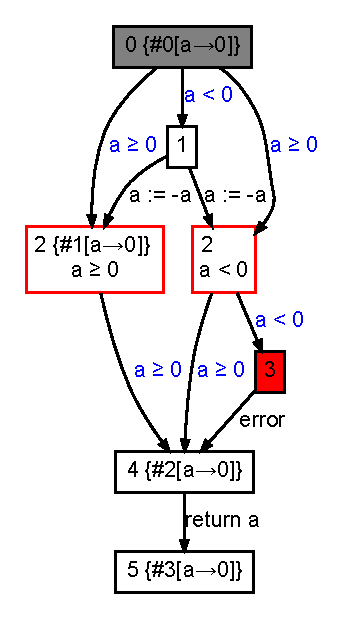
\includegraphics[height=\height]{{figs/subtleAbsOverflowFail/10test.graph.2.redboxes}.eps}
		\label{fig:dashInt:refinegraph:aftersplit}
	}
	\hfil
	\subfloat[New trace]
	{
		\includegraphics[height=\height]{{figs/subtleAbsOverflowFail/10test.graph.2.trace}.eps}
		\label{fig:dashInt:refinegraph:aftersplitnewtrace}
	}
	\caption
	{
		\protect\subref{fig:dashInt:refinegraph:beforesplit} shows an example region graph before refinement. \DASH tries to find a test that crosses the frontier marked with the red edge into the error region but the trace is infeasible and the graph is refined.
		\protect\subref{fig:dashInt:refinegraph:aftersplit} shows that region $2$ has been split and $\rho = 0 < a$ has been added to right region and $\neg \rho$ has been added to the left region.
		\protect\subref{fig:dashInt:refinegraph:aftersplitnewtrace} shows the trace found in the next iteration. The frontier edge has been pushed backwards.
	}
	\label{fig:dashInt:refinegraph}
\end{figure}

\section{\classname{ExtendFrontier}}
\label{sec:dashInt:extendFrontier}
\classname{ExtendFrontier} takes as input a trace $\tau_c$ constructed by \classname{ConvertToRegionTraceWithAbstractFrontier} and the procedure $P$. It either returns a test input that follows $\tau_c$, which effectively advances the frontier closer to the error region, or if such a test input does not exist, it returns a suitable refinement predicate that is used by \classname{RefineGraph} to eliminate the trace from the region graph. The pseudocode for \classname{ExtendFrontier} is given in \cref{alg:dashInt:extendFrontier}.

\classname{ExtendFrontier} starts by having the trace $\tau_c$ symbolically executed by calling \classname{ExecuteSymbolic}. The call results in the path constraint $\phi$, that models the requirements for executing the trace $\tau_c$ up to and including the frontier in the program $P$. The path constraint is passed to a SAT solver with a call to the \classname{IsSAT} procedure. The SAT solver attempts to find values for all the variables referenced in the constraint, such that the path constraint $\phi$ is satisfied. If the SAT solver succeeds in finding such values, then those are assigned to $t$. The test input $t$ includes all the arguments needed to call $P$ such that the trace $\tau_c$ is executed. The test input $t$ is returned as $\langle t,$ \code{true}$ \rangle$.

If the SAT solver was unable to satisfy the constraint then \unsat is returned by \classname{IsSAT}. The procedure \classname{RefinePred} is then called to compute a suitable refinement predicate $\rho$, which is returned as $\langle \unsat, \rho \rangle$ from \classname{ExtendFrontier}. 

The smaller sub procedure \classname{IsSAT} is described next whereas the larger \classname{ExecuteSymbolic} is described in \cref{sec:dashInt:executeSymbolic}. \classname{RefinePred} is described in \cref{sec:dashInt:refinePred}.

\begin{thesisalgorithm}
\caption{\classname{ExtendFrontier}($\tau_c, P$)}
\label{alg:dashInt:extendFrontier}
Returns:\\
$\langle t,$ \code{true}$ \rangle$, if the frontier can be extended; or\\
$\langle \unsat, \rho \rangle$, if the frontier cannot be extended

\begin{algorithmic}[1]
	\State $\phi := \classname{ExecuteSymbolic}(\tau_c, P)$
	\State $t := \classname{IsSAT}(\phi, P)$
	\If{$t = \unsat$}
		\State $\rho := \classname{RefinePred}(\tau_c)$
	\Else
		\State $\rho :=$ \code{true}
	\EndIf
	\State \Return $\langle t, \rho \rangle$
\end{algorithmic}
\end{thesisalgorithm}

\subsection{\classname{IsSAT}}
\label{sec:dashInt:isSat}
\classname{IsSAT} takes as input the path constraint $\phi$ and the procedure $P$. It then tries to find an assignment of values to the variables in the constraint, such that the constraint is satisfied. This is completed by using a theorem prover. The \DASH implementation in \YOGI and our own implementation of \DASH use the \Zthree theorem prover\footnote{\Zthree can be found at \url{http://z3.codeplex.com/}}.

If the constraint can be satisfied, then the values of all the variables are extracted and returned. If the constraint cannot be satisfied, then \unsat is returned to signal that no assignment to the variables could satisfy the constraint.

Sometimes the parameters of procedure $P$ are not mentioned in the path constraint $\phi$. This occurs when a parameter has not been used in any \code{assume} statements in the trace. However, an argument value is required for \classname{RunTest} to be able to concretely execute $P$. For this case, \classname{IsSAT} is given the procedure $P$ such that it can find the missing parameters and give them a default value of zero.

\section{\classname{ExecuteSymbolic}}
\label{sec:dashInt:executeSymbolic}
\classname{ExecuteSymbolic} is responsible for executing a trace $\tau_c$ symbolically and thereby computing the path constraint $\phi$, that should be feasible if and only if it is possible to execute $\tau_c$, including the frontier, in $P$. \classname{ExecuteSymbolic} maintains two pieces of information:

\begin{itemize}
	\item A map $\mathpzc{S}$ from symbolic variables to symbolic expressions. The notation $\mathpzc{S}:=\mathpzc{S}[f \mapsto q]$ overwrites $\mathpzc{S}$'s entry for $f$, such that $f$ now has the value $q$.
	
	\item A path constraint $\phi$, which accumulates individual path constraints and region predicates that are encountered during symbolic execution of $\tau_c$.
\end{itemize}

The pseudocode for \classname{ExecuteSymbolic} is provided in \cref{alg:dashInt:executeSymbolic}. The algorithm has two main parts: 1) initialization (lines 1-3) and 2) execution of the trace $\tau_c$ (lines 4-13). As can be seen, the auxiliary sub procedure \classname{SymbolicEval} is called throughout the code. The next section describes \classname{SymbolicEval} and thereafter the two main parts of \classname{ExecuteSymbolic} are presented in detail.

\begin{thesisalgorithm}
\caption{\classname{ExecuteSymbolic}($\tau_c=\langle S_0,\ldots,S_{k} \rangle, P$)}
\label{alg:dashInt:executeSymbolic}
Returns: $\phi$, the path constraint for reaching and crossing the frontier

\begin{algorithmic}[1]
	\State \Let $\langle \rho_0, \_ \rangle = S_{0}$
	\State $\mathpzc{S}:= [v \mapsto v_0 \mid v \in \classname{params}(P)]$
	\State $\phi := \classname{SymbolicEval}(\rho_0, \mathpzc{S})$
	\For{$i = 0$ \textbf{to} $k - 1$}
		\State $op := \classname{Op}(S_i, S_{i + 1})$
		\Match{$op$}
			\Case{\code{v := e}}
				\State $\mathpzc{S} := \mathpzc{S}[\code{v} \mapsto \classname{SymbolicEval}(\code{e}, \mathpzc{S})]$
			\EndCase
			\Case{\code{assume c}}
				\State $\phi := \phi \wedge \classname{SymbolicEval}(\code{c},\mathpzc{S})$
			\EndCase
		\EndMatch
		\State \Let $\langle \rho_{i+1}, \_ \rangle = S_{i+1}$
		\State $\phi := \phi \wedge \classname{SymbolicEval}(\rho_{i+1}, \mathpzc{S})$
	\EndFor
	\State \Return $\phi$	
	
\end{algorithmic}
\end{thesisalgorithm}

\subsection{\classname{SymbolicEval}}
\classname{SymbolicEval} takes two arguments, where the first is an expression, which can be a region predicate, a conditional expression, or an arithmetic expression. The second argument is the symbolic map $\mathpzc{S}$ which functions as is the environment that the first argument is to be evaluated under. The return value is a symbolically evaluated expression.

Example arguments to \classname{SymbolicEval} could be the region predicate or conditional expression $a>2$ and the map $\mathpzc{S}=\{a \mapsto 4\}$. In this example \classname{SymbolicEval} will replace $a$ with $4$, returning the predicate $4>2$.

An arithmetic example could be the expression $x+1$ and the map $\mathpzc{S}=\{x \mapsto (a + 4) * 3\}$. When the expression is symbolically evaluated it becomes $(a + 4) * 3 + 1$. Thus, \classname{SymbolicEval} simply substitutes variables mentioned in an expression with their symbolic expressions in the map $\mathpzc{S}$.

\subsection{Initialization of symbolic execution}
Initialization of \classname{ExecuteSymbolic} is completed by the lines 1-3 in \cref{alg:dashInt:executeSymbolic}. The region predicate $\rho_0$ is unpacked from region $S_0$ in line 1. An initial symbolic variable $v_0$ are assigned to each of the input variables $v \in \classname{params}(P)$ in line 2. Line 3 assigns the symbolically evaluated region predicate of $S_0$ to the path constraint $\phi$. Notice that in \DASHint, the predicate attached to region $S_0$ is always \code{true} due to how \classname{RefineGraph} handles refinement of the initial region described in \cref{sec:dashInt:refinegraph:initialRegion}. However, in \DASHcall initial regions can have non-\code{true} predicates assigned to them, and we therefore symbolically executes them in \DASHint as well.

\subsection{Executing the trace $\tau_c$}
The \code{for} loop in lines 4-13 is responsible for executing $\tau_c$, which includes the frontier. If the statement is an assignment statement \code{v := e}, then \code{e} is evaluated by \classname{SymbolicEval} and the resulting expression is used to update the symbolic map $\mathpzc{S}$ for the variable \code{v}. This occurs in lines 7-8. Lines 9-10 detect if the statement is an \code{assume c} statement, in which case the condition \code{c} is symbolically evaluated by \classname{SymbolicEval} and the result is added to the path constraint $\phi$. Additionally, all region predicates on the path are evaluated and added to the path constraint $\phi$ in line 12.

The path constraint $\phi$ is returned in line 14. At this point $\phi$ is the full path constraint for following the complete trace $\tau_c$. One should notice that if the frontier edge in $\tau_c$ is not included in $\phi$, then $\phi$ is guaranteed to be satisfiable. The reason is that the trace $\tau_c$ up until the frontier follows a concrete execution, which assures that the path constraint is satisfiable. An example of symbolic execution is presented in the next section.

\subsection{Examples of symbolic execution}
This section contains two examples for symbolic execution. The first example emphasizes what the symbolic map $\mathpzc{S}$ contains and how it is updated. The second example executes a trace and constructs the path constraint $\phi$ for it.

\subsubsection{Symbolic map example}
The first example is the symbolic execution of the code in \cref{fig:dashInt:executeSymbolicExample:example}. \Cref{fig:dashInt:executeSymbolicExample:symbolicmap} contains a table describing the symbolic map after each statement. The first entry in the table shows the initialization of the symbolic map $\mathpzc{S}$. The parameter $a$ is given the initial symbolic variable $a_0$. When the assignment in line 3 is executed, the symbolic map is updated by adding the mapping $q \mapsto a_0$. When executing \code{r := q + 1}, the symbolic map is updated again such that $r \mapsto a_0 + 1$. Notice that $q$ was symbolically executed, inserting the value $a_0$ in its place.

\begin{figure}
	\newsavebox{\executeSymbolicExample}
	\begin{lrbox}{\executeSymbolicExample}
\begin{lstlisting}[label=lst:executeSymbolicExample,numbers=left]
int inc(int a)
{
	int q := a;
	int r := q + 1;
	return r;
}
	\end{lstlisting}
	\end{lrbox}
	\centering
	\subfloat[Example program]
	{
		\usebox{\executeSymbolicExample}\label{fig:dashInt:executeSymbolicExample:example}
	}
	\hfil
	\subfloat[Memory map $S$]
	{
		\begin{tabular}{|l|l|}
			\hline
			Line number & $\mathpzc{S}$ after executing statement \\ \hline
			2 \textit{(initialization)}  & $\{a \mapsto a_0 \}$          \\ \hline
			3   & $\{a \mapsto a_0, q \mapsto a_0$ \}                    \\ \hline
			4   & $\{a \mapsto a_0, q \mapsto a_0, r \mapsto a_0 + 1$ \} \\ \hline
			5   & $\{a \mapsto a_0, q \mapsto a_0, r \mapsto a_0 + 1$ \} \\ \hline
		\end{tabular}
		\label{fig:dashInt:executeSymbolicExample:symbolicmap}
	}
	\caption
	{
		\protect\subref{fig:dashInt:executeSymbolicExample:example} shows an example program and \protect\subref{fig:dashInt:executeSymbolicExample:symbolicmap} shows the contents of the symbolic memory map $\mathpzc{S}$ after each line has been symbolically executed.
	}
	\label{fig:dashInt:executeSymbolicExample}
\end{figure}

\subsubsection{Symbolically executing a trace}
\label{sec:dashInt:executeSymbolic:exampleTrace}
This example will symbolically execute a trace in the \code{abs} procedure. The trace executed is $\tau_c = \langle 0, 1, 2{:}a{<}0 \rangle$, as shown in \cref{fig:dashInt:executesymbolic:trace}.

\begin{figure}
	\centering
	\subfloat
	{
		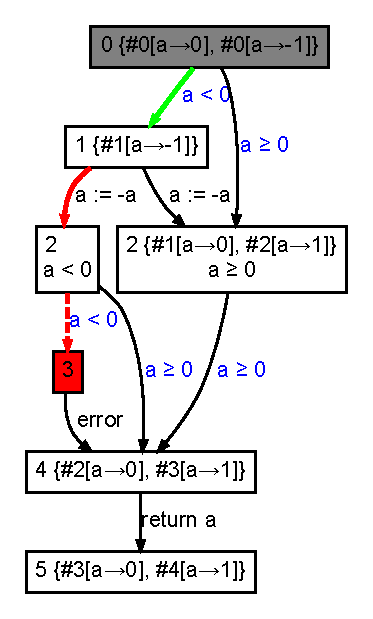
\includegraphics[height=7cm]{{figs/subtleAbsOverflowFail/16test.graph.4.trace}.eps}
	}
	\caption
	{
		The trace used as an example to show symbolic execution. The green part of the trace comes from following a concrete execution whereas no concrete states have crossed the red frontier statement. The red dashed line originates from the abstract error path, from which the trace was generated and is included only to show the direction the path was headed.
	}
	\label{fig:dashInt:executesymbolic:trace}
\end{figure}

First, initialization is performed. The first step is to initialize the symbolic map $\mathpzc{S}$ with initial symbolic variables for each parameter. The \code{abs} procedure only takes $a$ as an input parameter. The symbolic map $\mathpzc{S}$ is therefore initialized to $\{a \mapsto a_0\}$. The next step is to symbolically evaluate the region predicate for region $0$, which is \code{true}. After symbolic evaluation the expression is still \code{true}, which is the value $\phi$ is initialized to in line 3 of \classname{ExecuteSymbolic}.

The first iteration of the \code{for} loop starts by executing the green edge $(0, 1)$, which includes an \code{assume} $a<0$ statement. Symbolically evaluating the expression yields $a_0<0$. The expression is added to the path constraint $\phi$ which becomes \code{true} $\wedge~a_0 < 0$. The last step of the \code{for} loop is to symbolically evaluate the region predicate from region $1$, which is \code{true} and adding it to $\phi$ yields \code{true} $\wedge~a_0 < 0~\wedge$ \code{true}.

The second iteration of the \code{for} loop executes the edge $(1, 2{:}a{<}0)$ with the assignment \code{a := -a}. \classname{SymbolicEval} symbolically evaluates the expression $-a$, which results in $-a_0$ and assigning it to $a$ updates the symbolic map $\mathpzc{S}$ such that it becomes $\{a \mapsto -a_0\}$. The region predicate $a<0$ is then symbolically evaluated to $-a_0<0$ and added to $\phi$. The final path constraint $\phi$ returned by \classname{ExecuteSymbolic} is \code{true} $\wedge~a_0 < 0~\wedge$ \code{true} $\wedge~-a_0 < 0$. Simplifying the path constraint $\phi$, by removing the redundant \code{true} predicates from it, yields $a_0 < 0 \wedge -a_0 < 0$. This captures the constraints that need to be satisfied by a given value for $a_0$ if the trace seen in \cref{fig:dashInt:executesymbolic:trace} is to be followed.

\section{\classname{RefinePred}}
\label{sec:dashInt:refinePred}
\classname{RefinePred} is called by \classname{ExtendFrontier} when the path constraint $\phi$ for a trace $\tau_c$ has been found \unsat. Thus the trace is infeasible and \classname{RefinePred}'s task is to find a suitable refinement predicate that can be used by \classname{RefineGraph}.

\classname{RefinePred} takes as input the trace $\tau_c$ that has been found infeasible. This implies that the frontier could not be crossed. \classname{RefinePred} must find a suitable refinement predicate $\rho$ that eliminates any future concrete executions along $\tau_c$. The refinement predicate is used to split region $S_{k-1}$, the region before the frontier, into two new regions $S_{k-1}^*$ and $S_{k-1}^{**}$ as described in \cref{sec:dashInt:refinegraph}. The pseudocode for \classname{RefinePred} is provided in \cref{alg:dashInt:refinePred}. Lines 4-8 provide a loop optimization, which is explained in \cref{sec:dashInt:refinePred:loopOptimization}.

\begin{thesisalgorithm}
\caption{\classname{RefinePred}$(\tau_c= \langle S_0, \ldots, S_{k-1}, S_k\rangle)$}
\label{alg:dashInt:refinePred}
Returns: $\rho$, a suitable predicate for refinement.
\begin{algorithmic}[1]
	\State \Let $\langle \_, states_{k-1} \rangle = S_{k-1}$
	\State \Let $\langle \rho_k, \_ \rangle = S_k$
	
	\State $op := \classname{Op}(S_{k-1}, S_k)$
	\If{$op$ \matches \code{assume c}}
		\If{$k > 1 \wedge \forall s \in states_{k-1}: \classname{Eval}(\neg \rho_k, s)$ = \code{true}}
			\State \Return $\rho_k$
		\EndIf
	\EndIf
	\State \Return $\classname{WP}(op, \rho_k)$ 
\end{algorithmic}
\end{thesisalgorithm}

A suitable predicate $\rho$ must have the following characteristics with respect to the trace $\tau_c$, that has the frontier edge $(S_{k-1}, S_k)$, before it is a good candidate for a refinement predicate:
\begin{enumerate}
	\item All concrete executions that follow $\tau_c$ must satisfy $\neg\rho \wedge \rho_{k-1}$ at $S_{k-1}$. $S_{k-1}$ is the region before the frontier and $\rho_{k-1}$ is the region predicate of $S_{k-1}$.
	
	\item It is not possible to reach the region after the frontier $S_k$ for any execution that reaches $S_{k-1}^*$, which has the predicate $\neg\rho \wedge \rho_{k-1}$. Therefore the edge between $S_{k-1}^*$ and $S_k$ can be removed.
\end{enumerate}

Ignoring the loop optimization in lines 4-8, \classname{RefinePred} always returns the weakest precondition computed by the procedure \classname{WP}. The next section describes how the weakest precondition $\rho_{wp}$ is computed. After having introduced the weakest precondition we argue that $\rho_{wp}$ is a suitable predicate.

\subsection{Weakest precondition computed by \classname{WP}}
\label{sec:dashInt:wp}
The goal of the \classname{WP} procedure is to compute the weakest precondition for a postcondition $p$ and an operation $op$. It has two properties:
\begin{itemize}
	\item It is a precondition, such that if $\rho_{wp} = \classname{WP}(op, p)$ holds before $op$ then $p$ holds after $op$ has been executed.
	\item It is the weakest of all preconditions, such that for all other preconditions $P'$ that holds for $op$ and $p$, then $P'$ implies $\rho_{wp}$.
\end{itemize}

There are only two possible operations in \DASHint, namely assignments \code{v := e} and \code{assume c} statements.

For assignments, \classname{WP} is calculated by replacing the assigned variable \code{v} in $p$ with \code{e}, which is written as $p[\code{e}/\code{v}]$. Calculating the weakest precondition for the assignment \code{x := 4} with the postcondition $z > x$ proceeds like:
\begin{align*}
\classname{WP}(\code{x := 4}, z > x) \is& (z > x)[4/x]\\
	\is& z > 4
\end{align*}

For \code{assume c} statements, the condition \code{c} is added to $p$: \classname{WP}$\left(\text{\code{assume c}}, p\right)=\code{c}\wedge p$. For example:
\begin{align*}
\classname{WP}(\text{\code{assume} x > 4}, x < 10) \is& x > 4 \wedge x < 10
\end{align*}

Notice that the \DASH article uses a special procedure \classname{WP$_\alpha$} where aliasing is considered. \DASHint does not support pointers and therefore aliasing cannot occur which simplifies \classname{WP} considerably. 

The pseudocode for \classname{WP} is shown in \cref{alg:dashInt:wp}. We argue in the next section that the weakest precondition $\rho_{wp}$ is a suitable predicate.

\begin{thesisalgorithm}
\caption{\classname{WP}($op, p$)}
\label{alg:dashInt:wp}
Returns: $\rho_{wp}$, the weakest precondition for $op$, such that $p$ evaluates to \code{true} after executing $op$.

\begin{algorithmic}[1]
	\Match{$op$} 
		\Case{v := e}
			\State \Return $p[\code{e}/\code{v}]$
		\EndCase
		\Case{\code{assume c}}
			\State \Return $\code{c} \wedge p$
		\EndCase
	\EndMatch
\end{algorithmic}
\end{thesisalgorithm}

\subsection{The weakest precondition is a suitable predicate}
The classical weakest precondition $\rho_{wp}$ can be used as a suitable predicate: 

\begin{enumerate}
	\item We know that no execution of $\tau_c$ is able to cross the frontier since we were not able to find a test input with the SAT solver in \classname{ExtendFrontier}. Assume for contradiction that there exists an execution in $\tau_c$ that satisfies $\rho_{wp}$ at $S_{k-1}$, then that execution would be able to cross the frontier, by the definition of $\rho_{wp}$. The SAT solver would then have found the input, but the SAT solver did not find such an input. Therefore no concrete execution in $\tau_c$ satisfies $\rho_{wp}$ and consequently all concrete executions that follow $\tau_c$ must satisfy $\neg\rho_{wp}$ at region $S_{k-1}$.
	
	\item Let $s$ be a state that satisfies $\neg \rho_{wp}$ and let $\rho_k$ be the region predicate on region $S_k$. Assume for contradiction that $\rho_k$ is satisfied after executing the frontier operation $op$, when in the state $s$. Let then $P_s$ be a predicate that is only satisfied by $s$. $P_s$ is then a precondition for $op$ and $\rho_k$, due to the assumption that $s$ satisfies $\rho_k$ after having executed $op$. Since $P_s$ is a precondition, and $\rho_{wp}$ is the weakest precondition, then by the definition of a weakest precondition, $P_s$ implies $\rho_{wp}$, which means that $s$ must satisfy $\rho_{wp}$. This is a contradiction, since we assumed that $s$ satisfied $\neg \rho_{wp}$. Therefore no state can satisfy $\neg \rho_{wp}$ and satisfy $\rho_k$ after executing $op$, which was the frontier operation. The result is that there are no possible transitions from region $S_{k-1}$, with the predicate $\neg \rho_{wp}$ added, to region $S_k$.
\end{enumerate}

The definition of suitable predicates mentions the region predicate $\rho_{k-1}$ from region $S_{k-1}$. However, $\rho_{k-1}$ has been left out of the argumentation for $\rho_{wp}$ since any state that reaches $S_{k-1}$ must trivially satisfy $\rho_{k-1}$ because it is the region predicate.

The predicate $\rho_{wp}$, computed by the procedure \classname{WP}, is therefore a suitable predicate and can be returned for use in $\classname{RefineGraph}$.

\subsection{\classname{RefinePred} loop optimization}
\label{sec:dashInt:refinePred:loopOptimization}
As seen, the weakest precondition for an \code{assume c} statement \classname{WP}(\code{assume c}, $p$) is $\code{c} \wedge p$. During refinement of a loop, the condition of the loop or any other condition inside the loop will thus always be added for each round of the loop that the trace follows. However, there are properties where the work performed inside the loop is irrelevant for the safety property being checked. \DASH may try more and more iterations of the loop to reach the safety property, but as mentioned, sometimes the loop is irrelevant for the safety property. This can keep \DASH refining infinitely as we describe in \cref{sec:dashInt:challenges:infiniteRefinementWithLoopOptimziation}. 

To overcome this special case, \DASH uses a trick. When computing the refinement predicate for an \code{assume c} statement, \DASH tries to see if the region predicate $\rho_k$ from region $S_k$ is strong enough to be used as a refinement predicate. It thus tries to see if the \code{assume} condition \code{c} can be ignored.

Checking if the region predicate is strong enough is performed by evaluation. \DASH checks if each of the concrete states contained in $S_{k-1}$ satisfies the condition $\neg\rho_k$. If this is the case, then the region predicate may be able to satisfy the first condition of a suitable predicate.  Only the currently known states in $S_{k-1}$ are checked to see if they are moved to $S_{k-1}^*$ with $\neg\rho_k$, and thus not all states that can be obtained by following the trace $\tau_c$ are guaranteed to be moved. Thus the region predicate is not guaranteed to be a suitable predicate. The second condition of a suitable predicate is satisfied. No state that satisfies $\neg\rho_k$ is able to satisfy $\rho_k$. Thus, the region after the frontier cannot be reached from $S_{k-1}^*$ with $\neg\rho_k$ added.

The loop optimization is disallowed when refining an outgoing edge from the initial region. The reason why is described in \cref{sec:dashInt:challenges:howToImplementLoopOptimization:initialRegion}. The loop optimization could also result in an infinite refinement loop in \DASHcall, if the loop optimization is allowed on the initial region. This problem is described in \cref{sec:dashCall:infiniteRefineAtProc}.

The requirements for using the loop optimization is checked in \classname{RefinePred} lines 4 and 5, and if satisfied the region predicate is returned in line 6.

There are of course cases where the \code{assume c} condition is required for the analysis. If this is the case, then \DASH will find it at a later point. This is evident since if the same edge becomes a frontier at a later point, then a state must exist in the region before it. The state must satisfy the region predicate $\rho_k$ that was previously returned by the loop optimization. Thus, this time the region predicate $\rho_k$ cannot be strong enough to move all states to $S_{k-1}^*$. \classname{RefinePred} cannot use the loop optimization and is forced to use the weakest precondition returned by \classname{WP} wherein the \code{assume} condition is added.

\section{Complete example}
\label{sec:dashInt:completeExample}
At this point all the procedures that \DASHint uses have been presented. This section describes in detail how the \code{abs} procedure, shown again for convenience in \cref{fig:dashInt:complete:abs}, is analyzed by \DASHint. As should already be evident, \code{abs} contains an overflow error where passing the smallest value of an integer to \code{abs} will result in an error.

Initially the \DASH algorithm starts by constructing the region graph for the \code{abs} procedure. The resulting graph is shown in \cref{fig:dashInt:complete:initial}.

\begin{figure}
\newsavebox{\abs}
\begin{lrbox}{\abs}
\begin{minipage}[b]{0.25\textwidth}
\begin{lstlisting}[showlines=true,mathescape]
int abs(int a)
{
	if(a < 0)
		a = -a;
	assert a $\geq$ 0;
	return a;
}




\end{lstlisting}
\end{minipage}
\end{lrbox}
\def \height {6cm}
	\centering
	\subfloat[\code{abs} procedure]{\usebox{\abs}\label{fig:dashInt:complete:abs}}
	\hfil
	\subfloat[Initial]
	{
		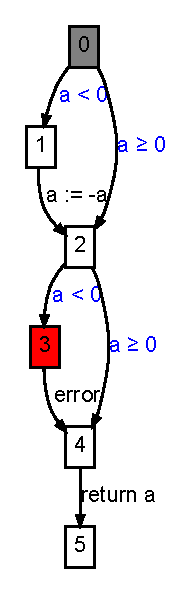
\includegraphics[height=\height]{{figs/subtleAbsOverflowFail/2test.graph.0.init}.eps}
		\label{fig:dashInt:complete:initial}
	}
	\hfil
	\subfloat[Error path]
	{
		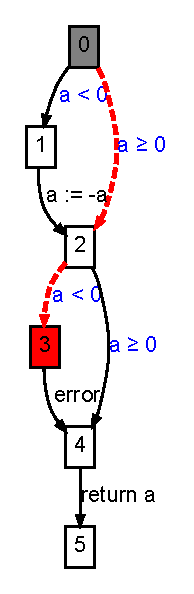
\includegraphics[height=\height]{{figs/subtleAbsOverflowFail/3test.graph.0.path}.eps}
		\label{fig:dashInt:complete:it1:path}
	}
	\hfil
	\subfloat[Trace]
	{
		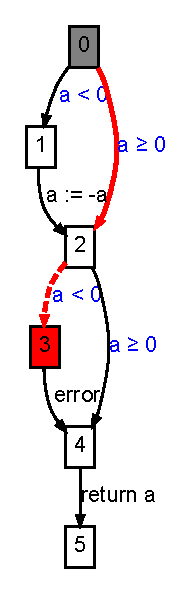
\includegraphics[height=\height]{{figs/subtleAbsOverflowFail/4test.graph.0.trace}.eps}
		\label{fig:dashInt:complete:it1:trace}
	}
	\hfil
	\subfloat[First test]
	{
		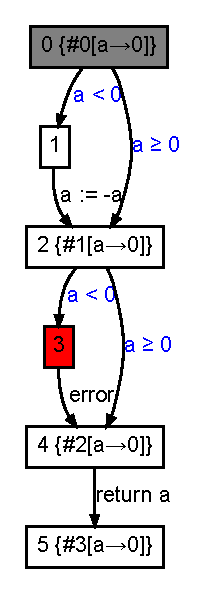
\includegraphics[height=\height]{{figs/subtleAbsOverflowFail/5test.graph.0}.eps}
		\label{fig:dashInt:complete:it1:traceIncluded}
	}
	\hfil
	\subfloat[Error path]
	{
		\includegraphics[height=\height]{{figs/subtleAbsOverflowFail/6test.graph.1.path}.eps}
		\label{fig:dashInt:complete:it2:path}
	}
	\hfil
	\subfloat[Trace]
	{
		\includegraphics[height=\height]{{figs/subtleAbsOverflowFail/7test.graph.1.trace}.eps}
		\label{fig:dashInt:complete:it2:trace}
	}
	\hfil
	\subfloat[Refinement]
	{
		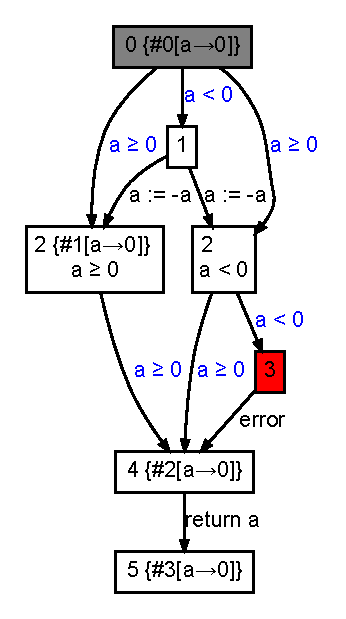
\includegraphics[height=\height]{{figs/subtleAbsOverflowFail/8test.graph.1}.eps}
		\label{fig:dashInt:complete:it2:refinement}
	}
	\hfil
	\subfloat[Trace]
	{
		\includegraphics[height=\height]{{figs/subtleAbsOverflowFail/10test.graph.2.trace}.eps}
		\label{fig:dashInt:complete:it3:trace}
	}
	\hfil
	\subfloat[4\textsuperscript{th} iteration]
	{
		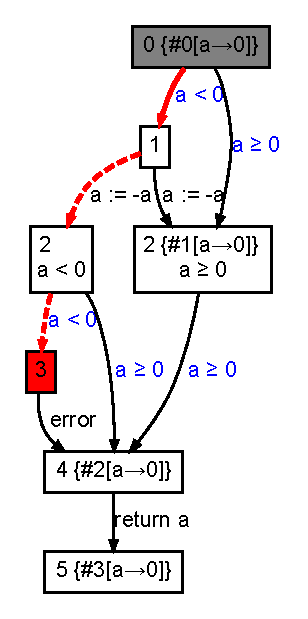
\includegraphics[height=\height]{{figs/subtleAbsOverflowFail/13test.graph.3.trace}.eps}
		\label{fig:dashInt:complete:it4:trace}
	}
	\hfil
	\subfloat[5\textsuperscript{th} iteration]
	{
		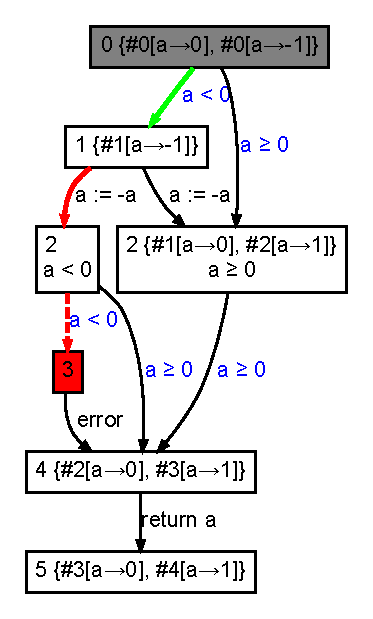
\includegraphics[height=\height]{{figs/subtleAbsOverflowFail/16test.graph.4.trace}.eps}
		\label{fig:dashInt:complete:it5:trace}
	}
	\hfil
	\subfloat[Error region reached]
	{
		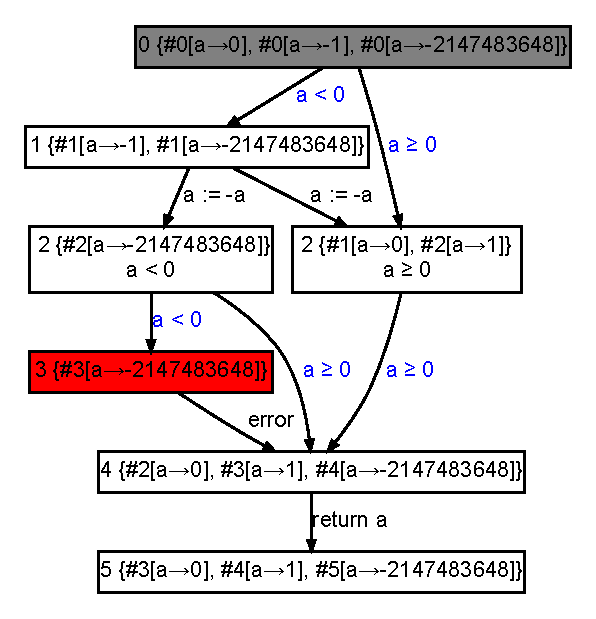
\includegraphics[height=\height]{{figs/subtleAbsOverflowFail/17test.graph.4.error}.eps}
		\label{fig:dashInt:complete:errorFound}
	}
	\caption
	{
		Example graphs for the \code{abs} procedure.
	}
	\label{fig:dashInt:complete}
\end{figure}

\subsection{First iteration -- Execute a test}
\DASHint starts by trying to find an abstract error path to an error region and finds $\tau = \langle 0,2,3 \rangle$ which is depicted in \cref{fig:dashInt:complete:it1:path} as red dashed lines. The abstract error path $\tau$ is converted by \classname{ConvertToRegionTraceWithAbstractFrontier} to a trace $\tau_c$ that follows a concrete execution trace. Such a concrete execution does not yet exist and as a special case, \classname{ConvertToRegionTraceWithAbstractFrontier} returns the trace $\tau_c = \langle 0,2 \rangle$ where the initial region $0$ is assumed to have a concrete state even though it does not. The trace is depicted in \cref{fig:dashInt:complete:it1:trace}. Notice that the dashed red line is not part of $\tau_c$, but it shows the path from which $\tau_c$ was generated.

At this point \DASHint calls \classname{ExtendFrontier} with the trace $\tau_c$ which in turn calls \classname{ExecuteSymbolic}. \classname{ExecuteSymbolic} starts by assigning all input variables a symbolic free variable, such that the symbolic map contains the mapping $a \mapsto a_0$. When symbolically executing $\tau_c$ it evaluates the \code{assume} $a \geq 0$ statement and inserts $a_0$ in place of $a$. Thus \classname{ExecuteSymbolic} returns the predicate $\phi = a_0 \geq 0$. No region predicates are added since these are all \code{true}.

\DASHint now needs to check if the predicate $\phi$ can be satisfied. It uses a SAT solver via the \classname{IsSAT} call. Since $a_0 \geq 0$ is satisfiable \classname{IsSAT} returns a valuation of the variables, and in this case it returns $[a_0 \mapsto 0]$. This makes \classname{ExtendFrontier} return with the result $\langle [a_0\mapsto0],$ \code{true}$\rangle$.

\classname{DashLoop} checks whether the test input could be generated by \classname{ExtendFrontier}, and in this case it could. The test input $[a_0\mapsto0]$ is given to \classname{RunTest}, which runs an instrumented version of \code{abs} that records the concrete states found during execution. 

\classname{RunTest} starts by adding the initial state to the first region. From the initial region it is possible to transition to either region $1$ or region $2$. \classname{RunTest} looks at the \code{assume} statements and the region predicates in the regions and evaluates the predicates. Since only $a \geq 0$ evaluates to \code{true}, the next region that \classname{RunTest} transitions to must be region $2$. \classname{RunTest} continues the execution by finding the regions that are reached and adding the concrete state to them, which results in \cref{fig:dashInt:complete:it1:traceIncluded}. Since a test was executed \classname{IsErrorRegionReached} is called to check if the error region was reached during testing. It returns \code{false} since no states are attached to the error region. This concludes the first iteration.

\subsection{Second iteration -- Infeasible trace refined}
We are now at a point where \DASHint have expanded the under-approximation of the program by executing a concrete test. As we shall see in this iteration, the under-approximation dictates where the graph is refined by having moved the frontier forward.

\DASHint starts by finding the same abstract error path as in the first iteration, which is depicted in \cref{fig:dashInt:complete:it2:path}. The only difference is that this graph contains concrete states, and this affects how \classname{ConvertToRegionTraceWithAbstractFrontier} creates the trace $\tau_c$. The first region with states, found by searching backwards in the abstract error path, is region $2$. The concrete execution that leads to region $2$ is spliced together with the step $\langle 2,3 \rangle$ which is the frontier, yielding $\tau_c=\langle 0,2,3 \rangle$ depicted in \cref{fig:dashInt:complete:it2:trace}. The green part follows a concrete execution while the red edge is the frontier. Notice that the frontier has been pushed forward by the \classname{RunTest} execution made in the first iteration.

At this point \DASHint calls \classname{ExtendFrontier} which in turn calls \classname{ExecuteSymbolic}. The initial value $a_0$ is then added for the input variable $a$ such that the symbolic map contains $a \mapsto a_0$. The first step in the trace adds $a_0 \geq 0$ to $\phi$ and the second step adds $a_0 < 0$. These predicates are clearly in conflict and \classname{IsSAT} therefore returns \unsat signaling that the predicates are unsatisfiable. The trace $\tau_c$ was therefore infeasible and no input could be generated that would follow it. Since the path leading up to the frontier is certainly feasible, as it followed a concrete execution, we know that it is the frontier edge that made the trace infeasible. At this point \classname{RefinePred} is called to generate a refinement predicate. \classname{RefinePred} calls \classname{WP} with the \code{assume} $a < 0$ statement and region $3$, which is the region after the frontier edge. \classname{WP} now finds the weakest precondition for the region predicate \code{true} in region $3$, that holds when executing the statement \code{assume} $a < 0$. In this case the weakest precondition is the \code{assume} statement predicate, namely $\rho = a < 0$. Notice that the loop optimization mentioned in \cref{sec:dashInt:refinePred} was not used in this case, since the region predicate for region 3 was \code{true}, which is not strong enough to be used as a refinement predicate.

The predicate $\rho$ found by \classname{RefinePred} is returned to \classname{DashLoop} which calls \classname{RefineGraph}. \classname{RefineGraph} splits region $2$ into two new regions, one with $\rho$ added and one with the negation $\neg\rho$ added. The region with $\neg\rho$ keeps all concrete states from region $2$ and the edge between it and region $3$ is removed. The resulting graph can be seen in \cref{fig:dashInt:complete:it2:refinement}.

\subsection{Third iteration -- Refinement}
\label{sec:dashInt:completeExample:thirdIteration}
The graph has been refined and an infeasible trace has been removed, however there are still paths that lead to the error region. We have shown the path, the trace and the resulting region graph for the first two iterations of \DASHint. For brevity the next iterations will only show the trace.

The path found by the procedure \classname{FindAbstractErrorPath} is $\tau = \langle 0, 2{:}a{<}0, 3 \rangle$ that is converted to the trace $\tau_c = \langle 0,2{:}a{<}0 \rangle$ depicted in \cref{fig:dashInt:complete:it3:trace}. This trace is infeasible since the first edge contains an \code{assume} $a \geq 0$ and the predicate in region $2$ specifies $a < 0$, which is the negation. For this case \classname{WP} returns $a<0\wedge a\geq 0$ as the refinement predicate, which is equivalent to \code{false}. The loop optimization is not attempted to be used by \classname{RefinePred}, since the edge is going out from the initial region. However, when refining the initial region, as performed by \classname{RefineGraph}, the edge is simply removed and the refinement predicate is not used. The refined graph, with the frontier edge removed, can be seen in \cref{fig:dashInt:complete:it4:trace}. Notice that the trace and path for the next iteration is also shown.

\subsection{Fourth iteration -- Execute a test}
In this iteration, \classname{ConvertToRegionTraceWithAbstractFrontier} returns the trace $\tau_c = \langle 0, 1 \rangle$ shown in \cref{fig:dashInt:complete:it4:trace}. \classname{ExecuteSymbolic} returns the path constraint $\phi = a_0 < 0$, which originates from the \code{assume} $a < 0$ statement between the regions.

When the path constraint is given to \classname{IsSAT} it returns the solution $[a_0 \mapsto -1]$ which will cross the frontier. Afterwards, \DASH calls \classname{RunTest} that runs the concrete test. When \classname{RunTest} reaches region 1, the statement \code{a := -a} is executed and $a$ becomes 1. Therefore \classname{RunTest} ends up in region $2{:} a {\geq} 0$, which leads away from the error region. This is not a problem, since we only required the test to reach the region after the frontier. The resulting graph, where \classname{RunTest} has completed its execution, can be seen in \cref{fig:dashInt:complete:it5:trace}. The error region has not been reached by concrete execution and therefore \DASH continues to the next iteration.

\subsection{Fifth iteration -- Reach the error region}
The previous iteration executed a test which added a concrete state to region $1$ that results in the frontier being pushed forward. The trace found is $\tau_c = \langle 0, 1, 2{:}a{<}0 \rangle$, which is depicted in \cref{fig:dashInt:complete:it5:trace}.

The trace is symbolically executed by passing it to \classname{ExecuteSymbolic}. Notice that this exact trace was used as an example for symbolic execution in \cref{sec:dashInt:executeSymbolic:exampleTrace}. The path constraint $\phi$ generated in the example, and thus for this trace, is $a_0 < 0 \wedge -a_0 < 0$.

When the path constraint is given to \classname{IsSAT} it finds the solution $[a_0 \mapsto -2{,}147{,}483{,}648]$, which is the smallest possible value of an 32 bit integer variable. One would think that $-(-2{,}147{,}483{,}648)$ is positive with the value of $2{,}147{,}483{,}648$, but the constraint requires that it is negative. The problem is that the largest possible value an integer variable can take is one less of $2{,}147{,}483{,}648$. The expression $-a_0$ actually overflows with exactly one, such that $-a_0=a_0$. Thus $a_0 \mapsto -2{,}147{,}483{,}648$ is a valid solution.

Calling \classname{RunTest} executes the test and the resulting graph is shown in \cref{fig:dashInt:complete:errorFound}. It can be seen that the error region now contains a concrete state and \classname{IsErrorRegionReached} thus returns \code{true}, making \DASH report that the error region is reachable with an input value of $-2{,}147{,}483{,}648$.

This concludes the complete example and the description of \DASHint. \DASHint is able to prune edges from the graph, such that it is not possible to reach the error region, and the program is then correct, or it might be able to direct a test such that the error region is reached, in which case the program violates the safety property with which it was instrumented. The last option is that \DASHint keeps analyzing forever.

The next sections describe the challenges and modifications we have made while implementing \DASHint.

\section{Challenges and modifications}
\label{sec:dashInt:challenges}
This section describes challenges we have encountered while implementing \DASHint and what modifications we have made to it compared to how \DASH is presented in the \DASH article~\cite{dash2010}.

\subsection{Combined data structure: Region graph}
Our presentation of \DASH uses a region graph for both the over- and under-approximation. The \DASH article keeps the concrete states in a so-called \textit{forest}. The reason that they term it a forest, is probably because they have nondeterminism in their programs and as such two executions with the same input variables may follow different execution paths. Since our programs do not contain any non-determinism we do not need a forest.

When converting an abstract error path to a trace we need to find the last region that contains a concrete state. This means that if we kept states in a separate data structure we would somehow need to know which region a given state belongs to. It therefore did not make sense to keep them divided from each other. Our presentation has been simplified significantly by having states directly attached to the regions in the region graph.

In fact, without non-determinism, it does not make sense to execute a test with the same input values more than once, and therefore we have an error-check in our implementation that makes sure that when executing a test, then the test has never been executed before.

\subsection{Ambiguity: Using $S_i$ both for regions and predicates}
The \DASH article uses $S_i$ both as a region, as in a trace $S_0, \ldots, S_n$, and as a predicate as in $S_0 \wedge \rho$. This is evident when looking at the use of $S_i$ in \cref{alg:dashInt:originalDash:refineGraph} and \cref{alg:dashInt:originalDash:executeSymbolic}. Since this is sometimes confusing we have removed such ambiguities from our presentation. Instead we explicitly unpack our regions $S_i$ to retrieve the region predicate $\rho_i$, or the states $states_{i}$, using the syntax:
\begin{align*}
	\text{\textbf{let} $\langle \rho_{i}, states_{i} \rangle = S_{i}$}
\end{align*}

\subsection{\classname{RefineGraph}: UNSAT regions have incoming edges removed}
\label{sec:dashInt:challenges:refineGraph:usatRegions}
The \DASH article refines the region graph directly inside the \classname{DashLoop} procedure. We have extracted the relevant pseudocode and presented it in \cref{alg:dashInt:originalDash:refineGraph}. Remember that states are not attached to the graph in the original \DASH article, and as such their algorithm does not move the states. 

\begin{thesisalgorithm}
\caption{\classname{RefineGraph$_{original}$}($\rho, \tau_c = \langle S_0, \ldots, S_{k-1}, S_k \rangle, G = \langle \Sigma_\simeq, \rightarrow_\simeq \rangle$)}
\label{alg:dashInt:originalDash:refineGraph}
Returns: $\langle \Sigma_\simeq, \rightarrow_\simeq \rangle$, the refined graph.
\begin{algorithmic}[1]
	\State $\Sigma_\simeq$ := 
	$(\Sigma_\simeq \setminus \{S_{k-1}\}$
	\State ~~~~~~~~~~~~~~~~$\cup \{S_{k-1} \wedge \rho, S_{k-1} \wedge \neg \rho\}$
	
	
	\State $\rightarrow \simeq$ := 
	$(\rightarrow \simeq \setminus \{ (S, S_{k-1}) \mid S \in \classname{Parents}(S_{k-1})\})$
	\State ~~~~~~~~~~~~~~~~~~$\setminus \{(S_{k-1}, S) \mid S \in \classname{Children}(S_{k-1})\}$
	
	
	\State $\rightarrow \simeq$ := $\rightarrow \simeq \cup \{(S, S_{k-1} \wedge \rho) \mid S \in \classname{Parents}(S_{k-1}$)$ \}$
	\State ~~~~~~~~~~~~~~~~~$\cup \{(S, S_{k-1} \wedge \neg \rho) \mid S \in \classname{Parents}(S_{k-1}$)$\}$
	\State ~~~~~~~~~~~~~~~~~$\cup \{(S_{k-1} \wedge \rho, S) \mid S \in \classname{Children}(S_{k-1}$)$ \}~$
	\State ~~~~~~~~~~~~~~~~~$\cup \{(S_{k-1} \wedge \neg \rho, S) \mid S \in  (\classname{Children}(S_{k-1}$)$\setminus \{S_k\})\}$ 
	
	
	\State \Return $\langle \Sigma_\simeq, \rightarrow_\simeq \rangle$
\end{algorithmic}
\end{thesisalgorithm}

The pseudocode in \cref{alg:dashInt:originalDash:refineGraph} is very specific in how the edges of the graph are updated. Nevertheless the graph is \textit{not} refined like shown in \cref{alg:dashInt:originalDash:refineGraph} in their \DASH implementation. 

We have found, by personal correspondence with the authors of \DASH that they deviate from their pseudocode in two fundamental ways:
\begin{enumerate}
	\item They simplify region predicates when the predicate is altered.
	\item If a region predicate is equivalent to \code{false} they remove the region from the graph.
\end{enumerate}

We have added those missing details to our \classname{RefineGraph} pseudocode as presented earlier in \cref{alg:dashInt:refinegraph}.

A question that rises is how \DASH simplifies the predicates. According to the authors they use a simplifying routine in the \Zthree\footnote{\Zthree can be found at \url{http://z3.codeplex.com/}} theorem prover to discover if a predicate is equivalent to \code{false}. However, there are two such routines, one which is a fast bottom-up rewriter and a second much more expensive implementation called \classname{ctx-solver-simplify}. The first can perform simple rewrites while the other is much more powerful and will simplify more complex predicates\footnote{Answer by \Zthree's author on \url{http://stackoverflow.com/a/14058292/477854}}. We have found that the first implementation is not good enough to simplify the predicates to \code{false} where needed, so they must be using the second. The \DASH article is very clear in that it uses only one SAT call for each iteration. However, simplifying a predicate using \classname{ctx-solver-simplify} is so slow, nontrivial and complex that we believe such a call is computationally equivalent to a SAT call. We have, in our implementation, frequently observed that \classname{ctx-solver-simplify} is as slow as many of our SAT calls. Timing information is provided in \cref{sec:dashImpl:sourcecode}.

The pseudocode in \cref{alg:dashInt:refinegraph} for \classname{RefineGraph} calls a \classname{Simplify} routine, but also uses the \classname{IsSAT} routine to check if the predicate is equivalent to \code{false}. In our implementation we use \classname{ctx-solver-simplify} for the \classname{Simplify} operation. We do this since we have found that the \classname{ctx-solver-simplify} routine has been able to simplify all predicates we have seen to \code{false} whenever \classname{IsSAT} says a predicate is unsatisfiable. However, the pseudocode uses the \classname{IsSAT} call since the contract for a satisfiability checker is to return \unsat when a predicate cannot be solved. It is not clear if \classname{ctx-solver-simplify} will always return \code{false} when a predicate is unsatisfiable. In our implementation we check that if \classname{ctx-solver-simplify} does not simplify to \code{false}, then \classname{IsSAT} has a solution to the predicate. The price is a significant slowdown of our implementation, but since this study is not about speed, we have kept it as an assertion.

\subsection{Confusing terminology: \textit{ordered path} and unused parts}
The \DASH article uses the term \textit{ordered path} $\tau_o$ about what we call the \textit{region trace with abstract frontier} $\tau_c$, or in short form the \textit{trace} $\tau_c$. We never found a reason to why they call $\tau_o$ \textit{ordered}. It is a list of regions that follows a concrete execution and regions from the rest of the abstract error path, but that does not make it \textit{ordered}. We have therefore chosen to use the term \textit{trace} instead.

We also slightly altered what a trace is. The \DASH article has an ordered path $\tau_o = \langle S_0, \ldots, S_{k-1}, S_k, \ldots S_n \rangle$ which is a concatenation of regions that follow a concrete execution $\langle s_0, \ldots, s_{k-1} \rangle$ and the rest of the abstract error path $\langle S_k, \ldots, S_n \rangle$. However, only the frontier edge from the abstract error path, located at $(S_{k-1}, S_k)$, is used by \DASH. We found it confusing to create a trace where the last part $\langle S_{k+1}, \ldots, S_n \rangle$ is never used, and as such we have chosen to only include the single edge that becomes the frontier. This has simplified the pseudocode in that we do not need to call an auxiliary \classname{Frontier} procedure to determine where the frontier edge is located in $\tau_o$. The frontier edge in our trace $\tau_c$ is always the last edge.

\subsection{\classname{ExecuteSymbolic}: assignments added to path constraints}
The original version of \classname{ExecuteSymbolic}, altered to how we present pseudocode, can be seen in \cref{alg:dashInt:originalDash:executeSymbolic}. Notice that they do not have local variables, only heap pointers. There are multiple differences between this code and how we presented \classname{ExecuteSymbolic} in \cref{alg:dashInt:executeSymbolic}. First of all they execute the trace up until the frontier in one loop and then execute the frontier statement for itself. We also need to do this in the \DASHcall algorithm, which is presented in \cref{ch:dashCall}. They return two predicates $\phi_1$ and $\phi_2$, but they are only used together in the call to \classname{IsSAT}. There is no technical reason to keep them apart. However, for presentation purposes it could be helpful to point out to the reader that $\phi_1$ is a constraint that can always be solved, since it originates from a concrete execution, but together with $\phi_2$ it might be unsatisfiable. We joined them together such that $\phi = \phi_1 \wedge \phi_2$.

\begin{thesisalgorithm}
\caption{\classname{ExecuteSymbolic$_{original}$}($\tau_c=\langle S_0,\ldots,S_{k} \rangle, P$)}
\label{alg:dashInt:originalDash:executeSymbolic}
Returns: $\langle \phi_1, \mathpzc{S}, \phi_2 \rangle$.

\begin{algorithmic}[1]
	\State $\mathpzc{S}:= [v \mapsto v_0 \mid *v \in \classname{inputs}(P)]$
	\State $\phi_1 := \classname{SymbolicEval}(S_0, \mathpzc{S})$
	\State $\phi_2 :=$ \code{true}
	\State $i := 0$
	\While{$i \neq k-1$}
		\State $op := \classname{Op}(S_i, S_{i + 1})$
		\Match{$op$}
			\Case{\code{*m=e}}
				\State $\mathpzc{S} := \mathpzc{S}[\classname{SymbolicEval}(\code{m}, \mathpzc{S}) \mapsto \classname{SymbolicEval}(\code{e}, \mathpzc{S})]$
			\EndCase
			\Case{\code{assume c}}
				\State $\phi_1 := \phi_1 \wedge \classname{SymbolicEval}(\code{c}, \mathpzc{S})$
			\EndCase
		\EndMatch
		\State $i:=i+1$
		\State $\phi_1 := \phi_1 \wedge \classname{SymbolicEval}(S_i, \mathpzc{S})$
	\EndWhile

	\State $op := \classname{Op}(S_{k-1}, S_k)$
	\Match{$op$}
		\Case{\code{*m := e}}
			\State $\phi_2 := \phi_2 \wedge *(\classname{SymbolicEval}(\code{m}, \mathpzc{S})) =  \classname{SymbolicEval}(\code{e}, \mathpzc{S})$
			\State $\mathpzc{S}' := \mathpzc{S}[\classname{SymbolicEval}(\code{m}, \mathpzc{S}) \mapsto \classname{SymbolicEval}(\code{e}, \mathpzc{S})]$
		\EndCase
		\Case{\code{assume c}}
			\State $\phi_2 := \phi_2 \wedge \classname{SymbolicEval}(\code{c}, \mathpzc{S})$
			\State $\mathpzc{S}' = \mathpzc{S}$
		\EndCase
	\EndMatch

	\State $\phi_2 := \phi_2 \wedge \classname{SymbolicEval}(S_k, \mathpzc{S}')$
	\State \Return $\langle \phi_1, \mathpzc{S}, \phi_2 \rangle$	

\end{algorithmic}
\end{thesisalgorithm}

The predicate that the authors of \DASH gives to \classname{IsSAT} is $\mu=\phi_1 \wedge \mathpzc{S} \wedge \phi_2$ where every entry in the symbolic map $\mathpzc{S}$ is seen as an equality predicate. Because the map $\mathpzc{S}$ is from before the frontier edge has been symbolically executed, they add the equality predicate for frontier assignments in line 18 in \cref{alg:dashInt:originalDash:executeSymbolic}. It makes no sense to include $\mathpzc{S}$ when we only consider local variables, and as such the constraint we give to \classname{IsSAT} is $\mu = \phi_1 \wedge \phi_2$ which is equivalent to our definition of $\phi$. We have not yet discovered why $\mathpzc{S}$ in $\mu$ is needed, but from personal correspondence with the authors, we believe it is related to heap aliasing constraints.

\subsection{Problem: Should the trace $\tau_c$ follow the path $\tau$}
\label{sec:dashInt:challenges:mustTraceFollowPath}
The quote below is from the \DASH article and it explains how they convert what we call an error path into a trace, which is what \classname{ConvertToRegionTraceWithAbstractFrontier} does:
\begin{thesisquote}{Page 8 in \DASH~\cite{dash2010}}
	The auxiliary function \classname{GetOrderedAbstractTrace} converts an arbitrary abstract trace $\tau$ into an ordered abstract trace $\tau_o$. This works by finding the last region in the abstract trace that intersects with the forest $F$, which we call $S_f$. The algorithm picks a state in this intersection and follows the \textit{parent} relation back to an initial state. This leads to a concrete execution $s_0, s_1, \ldots, s_{k-1}$ that corresponds to an abstract trace $S_0, S_1, \ldots, S_{k-1}$ where $S_{k-1} = S_f$. By splicing together this abstract trace and the portion of the abstract error trace from $S_f$ to $S_n$, we obtain an ordered abstract error trace. It is crucial that the ordered abstract error trace follows a concrete execution up to the frontier, as this ensures that it is a feasible trace up to that point.
\end{thesisquote}

From the quote it seems rather clear that to convert an error path to a trace one goes backwards in the path and finds the first region that contains a concrete state. However, we have seen instances where the trace found $s_0, s_1, \ldots, s_{k-1}$ does not follow the error path $S_0, S_1, \ldots S_n$.

A small example is shown in \cref{fig:dashInt:traceFollowPath}. The path found in \cref{fig:dashInt:traceFollowPath:path} is $\tau = \langle 0, 1, 3, 4 \rangle$ while the trace follows a different route $\tau_c = \langle 0, 1, 2, 1, 3, 4 \rangle$ shown in \cref{fig:dashInt:traceFollowPath:trace}. It seems counterintuitive that the trace follows a different set of edges compared to the path from which it is constructed. 

We were in doubt if the trace should always follow the path from which it was constructed. It led us to implement at version where the traces always followed the path. However, the implementation failed in numerous of our test cases due to timeouts and this is also evident for the path in \cref{fig:dashInt:traceFollowPath:path}. If the trace needs to follow the path, we can only generate a trace $\tau_c = \langle 0, 1, 3\rangle$ where the frontier is the edge $(1,3)$. However, the trace is clearly infeasible, since it is not possible to take zero iterations of the \code{while} loop. Eventually the \DASH algorithm will have refined the region graph such that a trace to the error region 4 can be created. However, if we change the \code{while} condition from $i < 1$ to $i < 1000$, then the algorithm becomes painfully slow. In this case it needs to refine the graph so many times, that only a trace that takes 1000 iterations of the loop leads to the error region. If we allow the trace to follow a path different from the abstract error path, then we can immediately generate a test by choosing the state that exists in region 3. This observation allows us to conclude that the trace $\tau_c$ is allowed to follow a different path compared to the error path $\tau$.

\begin{figure}
\newsavebox{\dashIntTraceFollowPathCode}
\begin{lrbox}{\dashIntTraceFollowPathCode}
\begin{minipage}[b]{0.25\textwidth}
\begin{lstlisting}[showlines=true]


void foo(int a)
{
	int i = 0;
	while(i < 1)
		i = i + 1;
	assert(a < 0);
}


\end{lstlisting}
\end{minipage}
\end{lrbox}
\def \scale {0.65}
	\centering
	\subfloat[Example code]
	{
		\usebox{\dashIntTraceFollowPathCode}
		\label{fig:dashInt:traceFollowPath:code}
	}
	\hfil
	\subfloat[Error path $\tau$]
	{
		\includegraphics[scale=\scale]{{figs/traceFollowPath/6test.graph.1.path}.eps}
		\label{fig:dashInt:traceFollowPath:path}
	}
	\hfil
	\subfloat[The trace $\tau_c$ found]
	{
		\includegraphics[scale=\scale]{{figs/traceFollowPath/7test.graph.1.trace}.eps}
		\label{fig:dashInt:traceFollowPath:trace}
	}
	\caption
	{
		\protect\subref{fig:dashInt:traceFollowPath:code} shows a small example where the code has been borrowed from \SYNERGY and altered. \protect\subref{fig:dashInt:traceFollowPath:path} shows a path in the region graph where one test with $a\mapsto0$ has been executed. The trace found is shown in \protect\subref{fig:dashInt:traceFollowPath:trace}. Notice that the trace does not strictly follow the path in \protect\subref{fig:dashInt:traceFollowPath:path}.
	}
	\label{fig:dashInt:traceFollowPath}
\end{figure}

\subsection{Problem: Which state to pick when creating traces}
\label{sec:dashInt:challenges:whichStateToPick}
The previous section described that when converting an abstract error path to a trace, one searches back in the path to find the first region that contains concrete states. The \DASH authors wrote the following about choosing a state in that region:

\begin{thesisquote}{Page 8 in \DASH~\cite{dash2010}}
	The algorithm \textbf{picks} a state in this intersection and follows the \textit{parent} relation back to an initial state.
\end{thesisquote}

Bold text has been added to highlight that the \DASH article is vague in how a state is picked. If there is only a single state in a region, then it is obvious that one should use that state to construct the trace from. However, it is unclear which state should be used to construct the trace when there are multiple to pick from. From a correctness perspective it does not matter which state is picked, eventually the algorithm will lead to the same answer. We have thought of multiple different strategies to pick the state:

\begin{itemize}
	\item Pick a random state
	\item Pick the last state (which our implementation does)
	\item Pick a state that enters the sought region
\end{itemize}

Since we did not know how to pick a state, we initially picked a random state as the state to generate the trace from. This works well for many test cases. However, there are cases where picking a random state seems counterintuitive.

\cref{fig:dashInt:randomStateBad} shows such an example. The code is shown in \cref{fig:dashInt:randomStateBad:code} and it should be clear that the \code{error} statement cannot be reached. At one point in \DASHint the path in  \cref{fig:dashInt:randomStateBad:path} needs to converted to a trace. There are 1001 states in region 2 from which a trace can be generated. All of them are infeasible, when the frontier edge $(2,4{:}a{=}0)$ is added, but it should be noted that one of them stands out. 1000 of the states are infeasible since they take less than the required iterations of the \code{while} loop. One state, the last state, takes the required 1000 iterations of the loop, but it is still infeasible because of the region predicate $a = 0$, which originates from region $4{:}a{=}0$.

In the above example it does not make a difference which state is picked, since all of them will result in the same refinement of the graph. However, it seems counterintuitive to choose traces that are clearly not feasible. We should pick a state that optimizes the chances for the trace to be feasible. Given the example we choose to always use the last state to generate the trace $\tau_c$ from. Using this implementation we get the trace $\tau_c = \langle 0,1,2,(3,2)^{1000},4 \rangle$ which is shown in \cref{fig:dashInt:randomStateBad:trace}. Using this heuristic we always choose to generate a trace from the newest test execution and therefore from the last iteration of loops.

\begin{figure}
\newsavebox{\dashIntRandomStateForTraceConstructionBad}
\begin{lrbox}{\dashIntRandomStateForTraceConstructionBad}
\begin{minipage}[b]{0.25\textwidth}
\begin{lstlisting}[mathescape,showlines=true]
void foo()
{
	int a = 1;
	int i = 0;
	while(i < 1000)
		i = i + 1;
	if(a == 0)
		error;
}
\end{lstlisting}
\end{minipage}
\end{lrbox}
\def \scale {0.56}
	\centering
	\subfloat[Example code]
	{
		\usebox{\dashIntRandomStateForTraceConstructionBad}
		\label{fig:dashInt:randomStateBad:code}
	}
	\hfil
	\subfloat[Error path $\tau$]
	{
		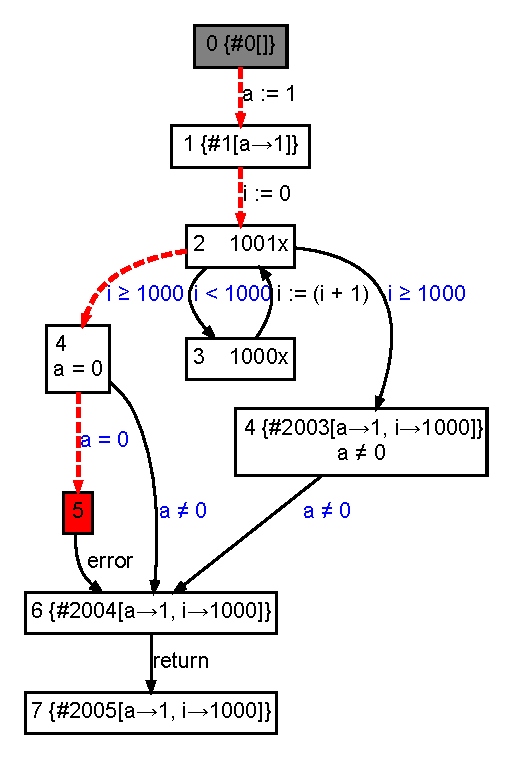
\includegraphics[scale=\scale]{{figs/synergyPass/9test.graph.2.path}.eps}
		\label{fig:dashInt:randomStateBad:path}
	}
	\hfil
	\subfloat[Many choices for $\tau_c$]
	{
		\includegraphics[scale=\scale]{{figs/synergyPass/10test.graph.2.trace}.eps}
		\label{fig:dashInt:randomStateBad:trace}
	}
	\caption
	{
		Example where many different traces can be generated by picking different states of region 2 in \protect\subref{fig:dashInt:randomStateBad:path}.
	}
	\label{fig:dashInt:randomStateBad}
\end{figure}

One idea that we had, but did not implement, was to look through all the states and find one that enters a region with the same region number as the region we seek to enter. For example, in \cref{fig:dashInt:randomStateBad:path} we seek to enter region 4 with the predicate $a=0$. However, no states actually lead there yet (as the frontier edge leads there). Instead, we can search for a state that is a good candidate for reaching the region, and if a state enters one of the regions with the region number 4, then it is a better candidate for reaching $4{:}a{=}0$. In this way, it is only the predicates on the regions that are different. Looking for states that enters a region with the same identification number might help in cases where it is not the last state that enters the sought region.

For the example in \cref{fig:dashInt:randomStateBad:path}, it would be the last state that is picked, since it enters region 4, even though the concrete state in it satisfies $a\neq0$, which is the negated predicate from region $4{:}a{=}0$. For this strategy we might have multiple states that enters region 4, in which case one has to either pick a random one or find a clever way to choose among them. However, since we did not implement this strategy, we are not sure if it would bring improvements over the strategy that picks the last state.

\subsection{Problem: Infinite refinement without loop optimization}
\label{sec:dashInt:challenges:infiniteRefinementWithLoopOptimziation}
Our pseudocode for \classname{RefinePred}, shown in \cref{alg:dashInt:refinePred}, includes a small test to see if a weaker predicate can be used as the refinement predicate for \code{assume c} edges. This loop optimization is mentioned in the evaluation section of the \DASH article, i.e. after the \DASH authors have described their algorithm. They write the following about the optimization:

\begin{thesisquote}{Page 12 in \DASH~\cite{dash2010}}
	When faced with an if-branch in a program, \DASH will perform an inexpensive test to see whether the \classname{WP}$_\alpha$ of a weaker predicate, one that ignores the branch condition, still satisfies the template described in Figure 9. The effect of this optimization is that we avoid getting ``stuck'' in irrelevant loops. We have left the consideration of more thorough generalization techniques for future work.
\end{thesisquote}

When implementing \DASHint we initially did not include the loop optimization because it was mentioned so late in the paper. However, when we discovered simple test cases that could not be solved without it, we felt forced to see if the loop optimization would help \DASH solve the test cases. It was not easy to implement, as we show in \cref{sec:dashInt:howToImplementLoopOptimization}.

A test case is shown in \cref{fig:dashInt:refineOptimization:code}. The code sets a variable $b$ to zero and takes exactly one iteration in the \code{while} loop, which does not affect $b$. Afterwards the \code{error} statement is executed if $b$ is equal to one. Since $b$ is never affected after the initial assignment the \code{error} statement can never be reached. However, without the optimization \DASH keeps analyzing infinitely and creates graphs such as the one seen in \cref{fig:dashInt:refineOptimization:forever}. We now show what difference the loop optimization makes to the presented example.

\begin{figure}
\newsavebox{\dashIntRefineOptimizationExample}
\begin{lrbox}{\dashIntRefineOptimizationExample}
\begin{minipage}[b]{0.22\textwidth}
\begin{lstlisting}[mathescape,showlines=true]
void test()
{
	int b = 0;
	int i = 0;
	while (i < 1)
		i++;
	if (b == 1)
		error;
}
\end{lstlisting}
\end{minipage}
\end{lrbox}
\def \scale {0.44}
	\centering
	\subfloat[Example code]
	{
		\usebox{\dashIntRefineOptimizationExample}
		\label{fig:dashInt:refineOptimization:code}
	}
	\hfil
	\subfloat[Before]
	{
		\includegraphics[scale=\scale]{{figs/loopOptimization/without/10test.graph.2.trace}.eps}
		\label{fig:dashInt:refineOptimization:before}
	}
	\hfil
	\subfloat[After without optimization]
	{
		\includegraphics[scale=\scale]{{figs/loopOptimization/without/11test.graph.2}.eps}
		\label{fig:dashInt:refineOptimization:without:after}
	}
	\hfil
	\subfloat[After with optimization]
	{
		\includegraphics[scale=\scale]{{figs/loopOptimization/with/11test.graph.2}.eps}
		\label{fig:dashInt:refineOptimization:with:after}
	}
	\hfil
	\subfloat[Later with optimization]
	{
		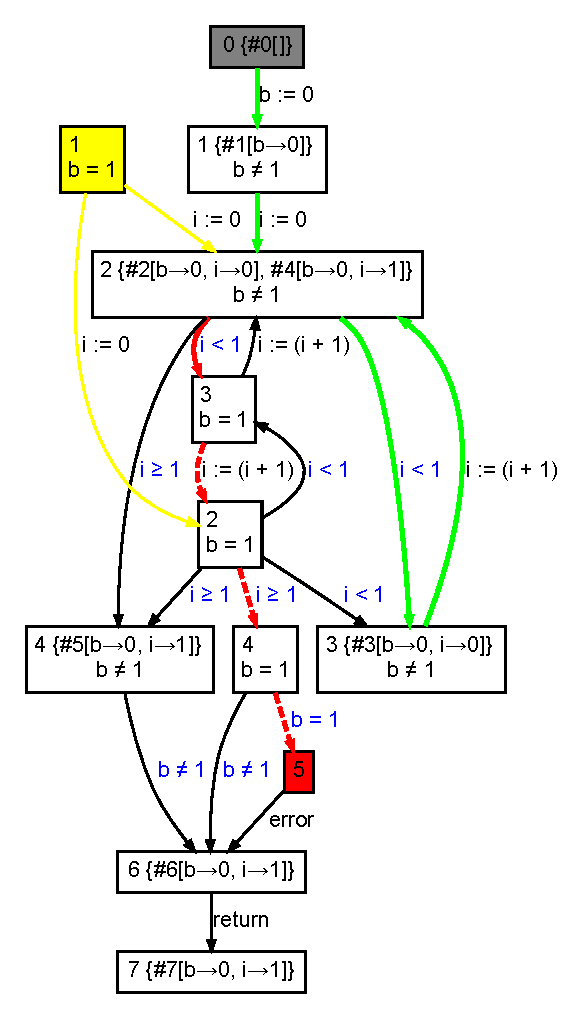
\includegraphics[scale=\scale]{{figs/loopOptimization/with/22test.graph.6.trace}.eps}
		\label{fig:dashInt:refineOptimization:with:later}
	}
	\hfil
	\subfloat[Later without optimization]
	{
		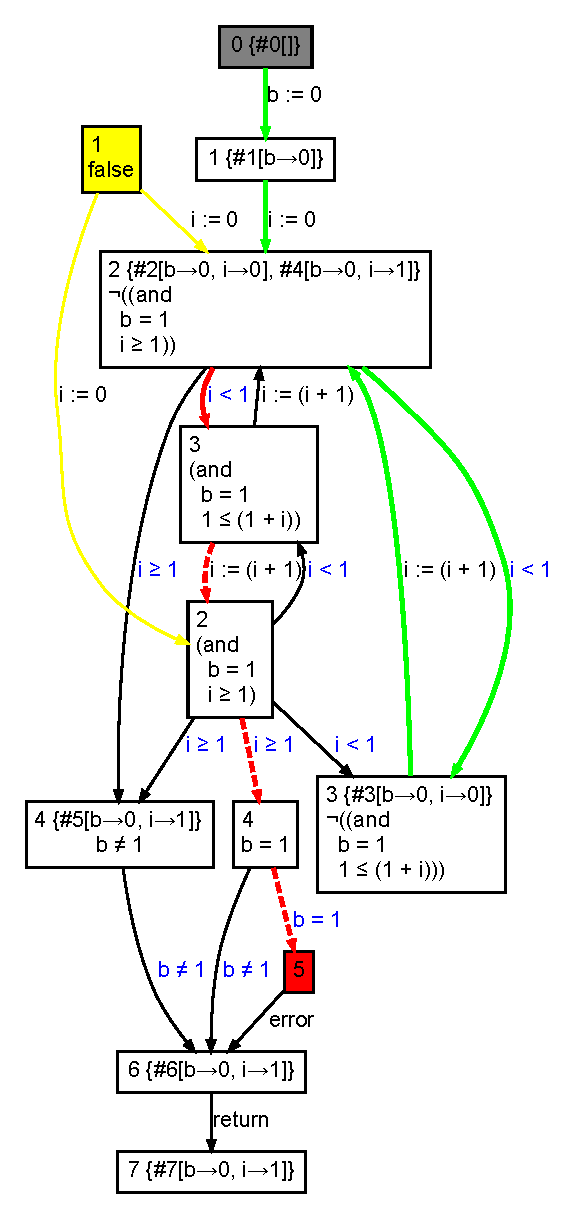
\includegraphics[scale=\scale]{{figs/loopOptimization/without/19test.graph.5.trace}.eps}
		\label{fig:dashInt:refineOptimization:without:later}
	}
	\caption
	{
		Region graphs showing how the loop optimization helps \DASH.
	}
	\label{fig:dashInt:refineOptimization}
\end{figure}

\cref{fig:dashInt:refineOptimization:before} shows a trace that is found when analyzing the code in \cref{fig:dashInt:refineOptimization:code}. So far the loop optimization has not made any differences. For this particular trace the refinement predicate returned by \classname{RefinePred} differs when the loop optimization is enabled.

Without the loop optimization, \classname{RefinePred} returns the refinement predicate $b = 1 \wedge i \geq 1$. This refinement predicate contains both the region predicate $b=1$ and the \code{assume} $i \geq 1$ condition. The graph returned by \classname{RefineGraph}, using the refinement predicate, is shown in \cref{fig:dashInt:refineOptimization:without:after}.

When the optimization is enabled the refinement predicate returned by \classname{RefinePred} is only the region predicate $b = 1$. It thus ignores the \code{assume} $i \geq 1$ condition. The optimization checks that the region predicate $b = 1$ is ``strong enough'' to be used as a refinement predicate. When the region before the frontier is split, the region that keeps the frontier edge must not contain any concrete states. This is to ensure progress is achieved. Using the weaker predicate results in the region graph in \cref{fig:dashInt:refineOptimization:with:after}. This shows that the optimization makes a difference, but so far, in this test case, we have not seen that it makes \DASHint terminate.

What makes \DASHint terminate is the impact that the refinement predicate has on a later iteration. Both versions will come to a trace that results in refining region 2. The traces are shown in \cref{fig:dashInt:refineOptimization:with:later} and \cref{fig:dashInt:refineOptimization:without:later}, with and without the optimization, respectively. The traces are the same, both with a frontier going out of region 2 and the traces are both infeasible since $b$ is required to be 1. The result of the two refinements are, however, very different. In this case the predicates returned by \classname{RefinePred} are different but since it does not make a difference here, we assume that they are the same. We assume that the refinement predicate is only the region predicate $b=0$. What matters here is that the predicates in region 2 are different. The one without the optimization has the predicate $\neg (b = 1 \wedge i \geq 1)$ and together with $b=0$ it becomes more complex. However, the version with the optimization has the predicate $b\neq0$ and together with $b=0$ one of the split regions gets the region predicate \code{false}. Therefore all ingoing edges to that region can be removed, which results in \cref{fig:dashInt:refineOptimization:with:complete}. Notice that with the optimization, \DASHint has completed the analysis. The error region is unreachable. The version without the optimization keeps trying to rule out the error region, but as \cref{fig:dashInt:refineOptimization:forever} shows, it tries more and more iterations of the loop, each of them being infeasible.

\begin{figure}
	\centering
	\subfloat[With optimization]
	{
		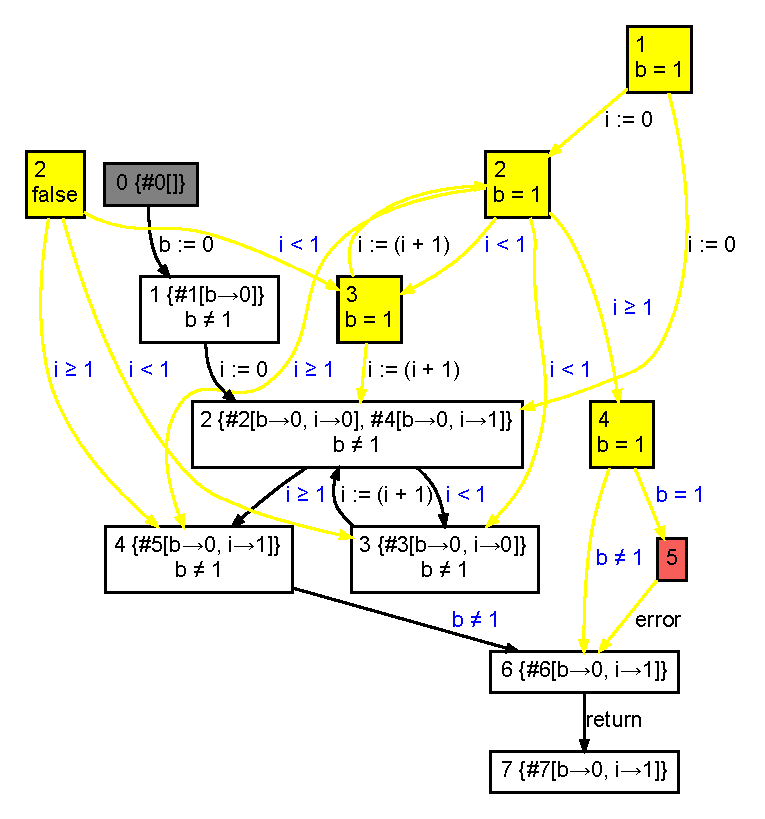
\includegraphics[scale=0.44]{{figs/loopOptimization/with/23test.graph.6}.eps}
		\label{fig:dashInt:refineOptimization:with:complete}
	}
	\hfil
	\subfloat[Without optimization]
	{
		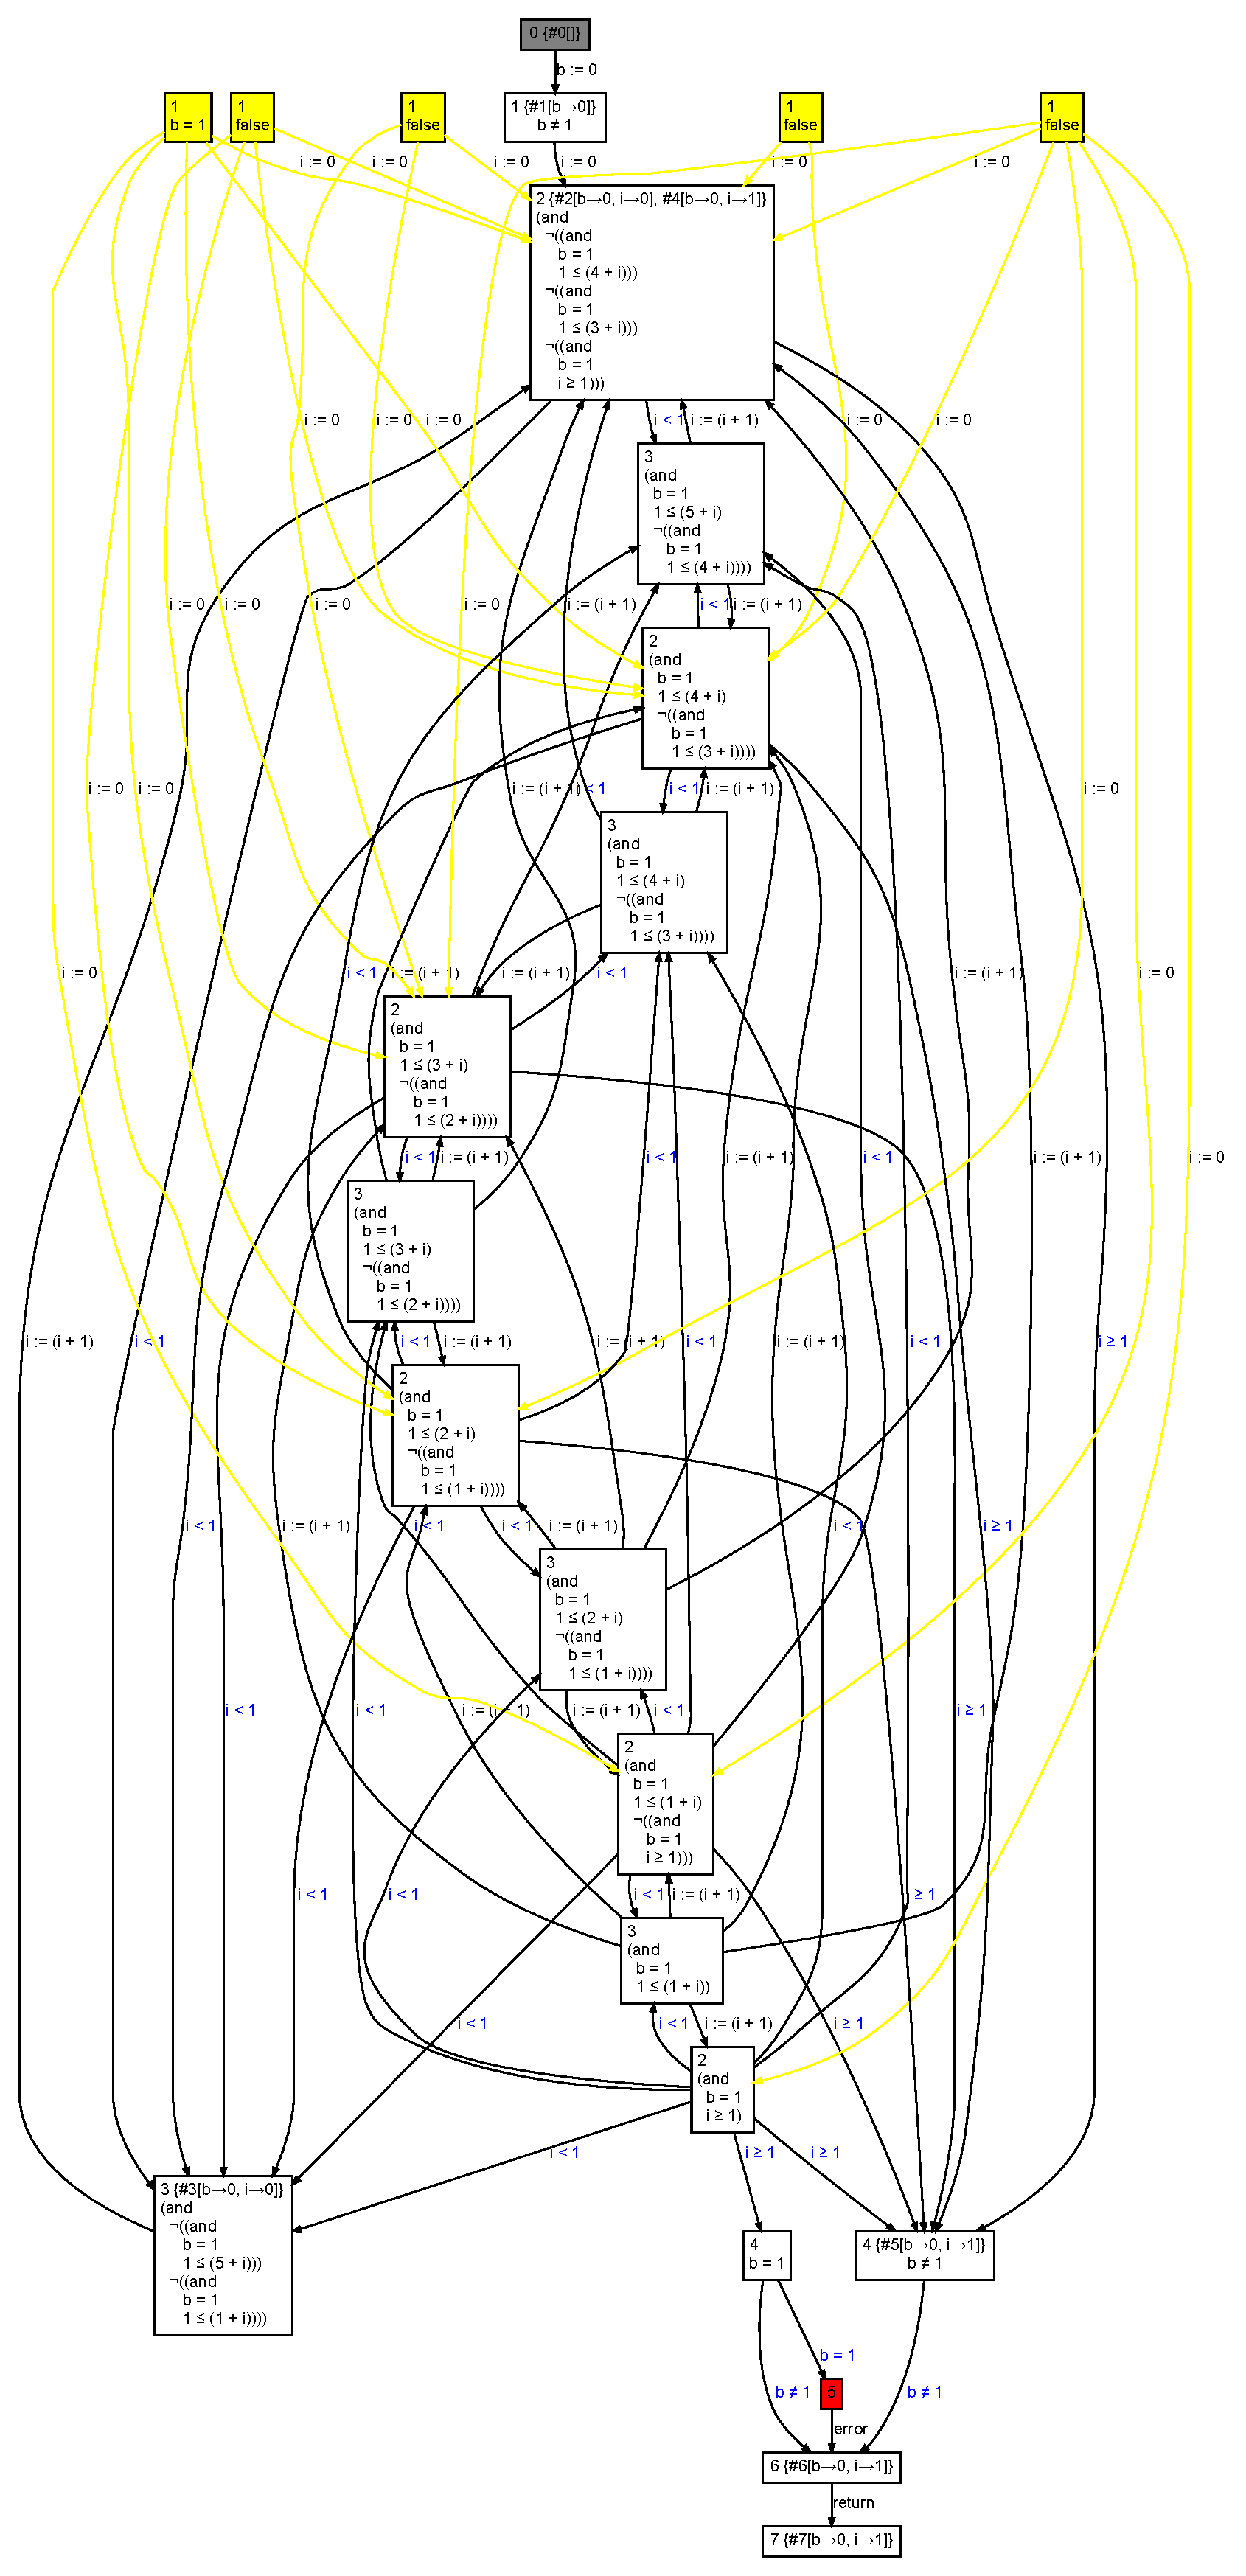
\includegraphics[scale=0.25]{{figs/loopOptimization/without/56test.graph.17}.eps}
		\label{fig:dashInt:refineOptimization:forever}
	}
	\caption
	{
		\protect\subref{fig:dashInt:refineOptimization:with:complete} shows that with the \classname{RefinePred} loop optimization, analysis ends contrary to without the optimization, which results in larger and larger graphs such as \protect\subref{fig:dashInt:refineOptimization:forever}.
	}
\end{figure}

We were a bit surprised that such a simple example could not be handled by \DASH without the loop optimization, which was mentioned as a side note in their evaluation section. We were especially surprised since \SYNERGY, the algorithm that \DASH builds on, boasts that it is very effective in generating a test for a very similar example, namely where the \code{while} condition is changed to $i<1000$ and where $b$ is a parameter of the \code{test} procedure\footnote{Page 119, Figure 1 in \SYNERGY~\cite{synergy2006}}. In that example the \code{error} statement can easily be reached (by calling \code{test} with $b\mapsto1$). By altering the example and making the \code{error} statement unreachable, we caused \DASH to iterate forever.

In the example given in \cref{fig:dashInt:refineOptimization:code}, the \code{while} loop is irrelevant to the $b$ variable, and therefore also to the instrumented safety property being checked. However, if the loop calculates something which is then asserted afterwards, then \DASH can still be brought to its knees. The example code in \cref{fig:dashInt:refineOptimizationCannotCopeExample} makes \DASH analyze forever, even with the optimization.

\begin{figure}
\newsavebox{\dashIntRefineOptimizationCannotCopeExample}
\begin{lrbox}{\dashIntRefineOptimizationCannotCopeExample}
\begin{minipage}[b]{0.65\textwidth}
\begin{lstlisting}[mathescape,showlines=true]
void test(int a)
{
    int k = 0;
    for (int i = 1; i < a $\wedge$ i < 10; i++)
        k += i;
    if (k == 2) // Not possible
        error;
}
\end{lstlisting}
\end{minipage}
\end{lrbox}
	\centering
	\usebox{\dashIntRefineOptimizationCannotCopeExample}
	\caption
	{
		\DASHint never halts when analyzing the \code{test} procedure.
	}
	\label{fig:dashInt:refineOptimizationCannotCopeExample}
\end{figure}

The \DASH authors already know this is a problem for the algorithm since they left this problem for future work:
\begin{thesisquote}{Page 13 in \DASH~\cite{dash2010}}
	We have left the consideration of more thorough generalization techniques for future work.
\end{thesisquote}

We also had trouble interpreting how their optimization should be implemented, as the next section shows.

\subsection{Problem: How to implement loop optimization}
\label{sec:dashInt:howToImplementLoopOptimization}
The above section found that the loop optimization is important and that it is needed for even trivial cases. However, we had problems in interpreting how it should be implemented. As a reminder, they wrote:

\begin{thesisquote}{Page 12 in \DASH~\cite{dash2010}}
	When faced with an if-branch in a program, \DASH will perform an inexpensive test to see whether the \classname{WP}$_\alpha$ of a weaker predicate, one that ignores the branch condition, still satisfies the template described in Figure 9. This can be done by evaluation, and does not require a theorem prover call.
\end{thesisquote}

Notice that for \DASHint \classname{WP}$_\alpha$ is equivalent to \classname{WP} since \DASHint do not have pointers and \classname{WP}$_\alpha$ is used to add aliasing constraints. Thus the ``the weaker predicate, one that ignores the branch condition'' must in \DASHint be the predicate from the region after the frontier since ignoring the branch condition in \classname{WP} yields the unmodified region predicate. However, there are still two main problems with their paragraph:

\begin{itemize}
	\item Figure 9 in the \DASH article is not very descriptive. It shows a split of a region into two. So the phrase ``satisfies the template described in Figure~9'' is not very helpful.
	
	\item It is unknown what test it is that they perform when they mention ``perform an inexpensive test''. It is clearly done by evaluation, but it is unknown what is evaluated.
\end{itemize}

In another section they refer to Figure~9 and define what they call a \textit{template-based refinement}. We believe this is what they are trying to refer to when they refer to Figure~9. The next question is what their ``inexpensive test'' is. When defining their \textit{template-based refinement} they define what a suitable predicate is and what requirements there are to it. We believe that their ``inexpensive test'' is to check if the region predicate alone is a suitable predicate. If this is the case, we have no idea why they did not write that. However, personal correspondence with the authors has verified that this is the case:

\begin{thesisquote}{Personal correspondence by email on the 18\textsuperscript{th} of March 2014.}
	We just check whether the resulting predicate still satisfies the conditions of a suitable predicate. If so, we use it. Otherwise, we fall back on the actual suitable predicate obtained by taking the if-condition into account.
\end{thesisquote}

The authors of \DASH write that for $\rho$ to be a suitable predicate it is required that \textit{all possible concrete states obtained by executing $\tau_c$ up to the frontier must belong to the region ($S\wedge\neg\rho$)}. Here ($S\wedge\neg\rho$) is the region with $\neg\rho$ added to it after splitting the region $S$, which we have called $S_{k-1}$.

The question is then how they perform an inexpensive test, using evaluation, to see whether the region predicate moves all the possible concrete states obtained by executing $\tau_c$ up to the frontier to the region with $\neg\rho$ added.

We can only think of one possible solution, namely that they test that the region predicate moves all \textit{known} states to the region with $\neg\rho$ added. This is how we have implemented the optimization, which is evident in lines 4-8 of \classname{RefinePred} in \cref{alg:dashInt:refinePred}. In this case it is not always the case that all the possible concrete states obtained by executing $\tau_c$ up to the frontier are moved correctly. We cannot see how we can ensure that all states that can be obtained by a trace $\tau_c$ is moved without using a theorem prover call. Thus our solution does not always return a suitable predicate. When we wrote to the authors of \DASH about this problem, they replied:

\begin{thesisquote}{Personal correspondence by email on the 5\textsuperscript{th} of April 2014.}
	In our implementation, we just check whether the concrete state (used to define the frontier etc.) satisfies $\neg\rho$ and that suffices for our purpose.
\end{thesisquote}

Thus checking that all \textit{known} concrete states are moved should suffice. The next section describes a situation where the predicate found is not a suitable predicate.

\subsubsection{Problem with the initial region not containing any states}
\label{sec:dashInt:challenges:howToImplementLoopOptimization:initialRegion}
When we implemented the above solution, we found cases where requiring that all known states were moved to the correct region was not enough. A special case is when refining the initial region when no concrete tests have yet been executed. In this case, no concrete states exist in the initial region and all states can thus be moved by any predicate. This can be a problem because the region after the frontier might only contain \code{true} as its predicate. One cannot refine anything with \code{true}.

The problem is depicted in \cref{fig:dashInt:problems:refineInitialRegionWithOptimizationAndNoStates}. To create such a graph an \code{if} statement must be the first statement and the condition must be equivalent to \code{false}. As can be seen the initial region contains no states and the error region after the frontier contains only the region predicate \code{true}. The trace is found infeasible. All states, which are none in this case, can be moved by the region predicate \code{true} from region 2, and thus \classname{RefinePred} will return it as the refinement predicate. We solved this problem by disallowing the use of the loop optimization on edges going out of the initial region. The initial region is the only region that can have a frontier edge going out of it while not having any states attached to it.

Initially we solved the problem by simply requiring that at least one state had to exist in the region. However, for reasons related to \DASHcall, as described in  \cref{sec:dashCall:infiniteRefineAtProc}, it was required that suitable predicates were always used to refine the initial region.

If we had continued and refined the initial region by splitting it, the region graph in \cref{fig:dashInt:problems:refineInitialRegionWithOptimizationAndNoStatesAfterRefine} would be obtained. Notice that no progress has been achieved in this graph. The same frontier exists and when refining it, the initial region is split resulting in three initial regions. This process will continue infinitely and therefore it simply does not make sense to use \code{true} as a refinement predicate.


\begin{figure}
\def \scale {0.7}
	\centering
	\subfloat[]
	{
		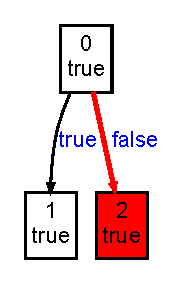
\includegraphics[scale=\scale]{figs/refinePredNoStates/before.eps}
		\label{fig:dashInt:problems:refineInitialRegionWithOptimizationAndNoStates}
	}
	\hfil
	\subfloat[]
	{
		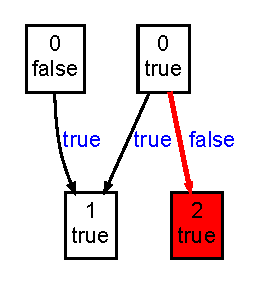
\includegraphics[scale=\scale]{figs/refinePredNoStates/after.eps}
		\label{fig:dashInt:problems:refineInitialRegionWithOptimizationAndNoStatesAfterRefine}
	}
	\caption
	{
		\protect\subref{fig:dashInt:problems:refineInitialRegionWithOptimizationAndNoStates} shows an infeasible trace where the initial region contains no states. Refining it by splitting the initial region with the refinement predicate \code{true} results in \protect\subref{fig:dashInt:problems:refineInitialRegionWithOptimizationAndNoStatesAfterRefine}. No progress has been made in \protect\subref{fig:dashInt:problems:refineInitialRegionWithOptimizationAndNoStatesAfterRefine} compared to \protect\subref{fig:dashInt:problems:refineInitialRegionWithOptimizationAndNoStates}.
	}
\end{figure}

\subsection{Problem: What happens when splitting the initial region}
\label{sec:dashInt:challenges:initialRegion}
The \classname{RefineGraph} pseudocode in \cref{alg:dashInt:refinegraph} removes edges from the initial region if they are found infeasible. This ``optimization'' is not mentioned in the \DASH article, but is a solution we found ourselves.

The \DASH article does not describe what happens when an initial region is refined. If an initial region is handled in the exact same manner as any other region, then the process of refining an initial region is shown in \cref{fig:dashInt:problems:refineInitialRegion:noSpecialCase}. The red frontier at the initial region before refinement is found infeasible and the initial region is refined with the refinement predicate $\rho$. This results in the graph after the arrow $\longrightarrow$. Notice that there have been no changes made for region 1 and 2, they can still be reached with any state that could reach it before the refinement. This is evident since to reach region 1 or 2, one has to go through one of the initial regions, which means that the initial state must satisfy the predicate $\neg\rho \vee \rho$. But that predicate is equivalent to \code{true}, and thus no changes have been made for them.

\begin{figure}
\def \scale {0.7}
	\centering
	\subfloat[No special case handling]
	{
		$\vcenterimage{figs/initialRegionRefine/before.eps}{\scale}
		\vcenterarrow
		\vcenterimage{figs/initialRegionRefine/after.eps}{\scale}$
		\label{fig:dashInt:problems:refineInitialRegion:noSpecialCase}
	}
	\hfil
	\subfloat[Special case: remove edge]
	{
		$\vcenterimage{figs/initialRegionRefine/before.eps}{\scale}
		\vcenterarrow
		\vcenterimage{figs/initialRegionRefine/afterRemoveEdge.eps}{\scale}$
		\label{fig:dashInt:problems:refineInitialRegion:specialCase}
	}
	\caption
	{
		Two strategies used to refine the initial region. Region graphs are shown before and after refinement.
	}
	\label{fig:dashInt:problems:refineInitialRegion}
\end{figure}

However, notice that the red frontier $(0{:}\rho, 3)$ after refinement is still infeasible. The reason is that it was found infeasible on the left, and since the requirements have only grown, it is still infeasible. Thus when refining the initial region, when it has no incoming edges, then the edge could be removed instead of adding predicates and maintaining multiple initial regions. This is the process depicted in \cref{fig:dashInt:problems:refineInitialRegion:specialCase}. The edge is simply removed. This is the strategy we have implemented.

Initially, we refined the initial region using the first strategy shown in \cref{fig:dashInt:problems:refineInitialRegion:noSpecialCase}, but where only the left region was marked as an initial region. The right one was ignored and thought to be unreachable. For all cases in \DASHint, the refinement predicate $\rho$ is \code{false} when refining the initial region. It will always be \code{false} because \classname{RefinePred} is disallowed to use the loop optimization on edges going out of the initial region (which contains no predicates), and thus it always uses \classname{WP} to construct the refinement predicate.

However, in \DASHcall, there are cases where the refinement predicate is not \code{false}. This is because the initial region can contain a predicate, which is not \code{true}, when analyzing sub procedures. A concrete example from \DASHcall can be seen in \cref{fig:dashCall:extendFrontier:extractRefinePred}, where the initial region is refined with a predicate that is not \code{false}. Splitting the initial region, as in \cref{fig:dashInt:problems:refineInitialRegion:noSpecialCase}, without marking the right region as an initial region, suddenly makes region 1 and 2 only reachable when the predicate $\neg\rho$ is satisfied, which is clearly a wrong refinement. We therefore needed to maintain either multiple initial regions or, when refining the initial region, remove the frontier edge such that only a single initial region exists. We chose the last option as it generated cleaner graphs.

%%%%%%%%%%%%%%%%%%%%%%%%%%%%%%%%%%%%%%%%%%%%%%%%%%%%%%%%%%%%%%%%%%%%%%%

\chapter{Interprocedural analysis with DASH$_{call}$}
\label{ch:dashCall}
In this chapter we present \DASHcall that adds interprocedural analysis on top of \DASHint.

The allowed program statements are extended with assignments of procedure calls \code{v := f}$(a_0, a_1, \ldots, a_n)$ and \code{return e} statements. However, the \code{error} statement is restricted to the main procedure $P$. Thus, \code{error} statements in sub procedures are not supported primarily due to how \classname{FindAbstractErrorPath} works. This is explained further in \cref{sec:dashCall:FindAbstractErrorPath}. Procedure calls \code{f}$(a_0, a_1, \ldots, a_n)$ that are not part of an assignment are not supported, since procedures are side effect free, due to the lack of global state, pointers, call by value semantics, and the fact that \code{error} statements are not allowed in sub procedures. The procedure call could therefore be removed, without changing the semantics, in a preprocessing step. State changed in a sub procedure must thus be propagated back through a return value. For the rest of the chapter, a \textit{procedure call} will refer to a procedure call that is part of an assignment. 

\DASHcall analyzes a complete program $\mathpzc{P}$ where each procedure has its own region graph. The \DASHcall version of \classname{DashLoop} takes as input the program $\mathpzc{P}$, a set of region graphs $\mathpzc{G}$ and the main procedure $P$. Special care must be taken when \DASHcall encounters a procedure call as the frontier edge. The main idea is to recursively invoke \classname{DashLoop} on the invoked procedure, but restraining its input to the context it is called in, and instrumenting it with a safety property that depends on crossing the frontier. We will explain this in detail when describing \classname{ExtendFrontier} in \cref{sec:dashCall:extendFrontier}.

\classname{ExecuteSymbolic} also needs to be modified such that it can execute a trace over a procedure call edge. At that point it needs to execute a trace through the invoked procedure. We describe \classname{ExecuteSymbolic} for \DASHcall in \cref{sec:dashCall:executeSymbolic}.

The \DASHcall implementation is able to handle recursive and mutually recursive procedures if the input value that determines the recursion depth is bound to a constant, ex. \code{fib(3)} or \code{fib(x)}, where x is assigned a constant value earlier. However it is not able to handle recursive procedures, where the recursion depth is dependent on a symbolic input value, e.i. $x_0$. We elaborate on recursive procedures in \cref{sec:dashCall:challenges:recursiveProcedures}.

We use a running example in this chapter to illustrate the inner details of how \DASHcall behaves. The example code is shown in \cref{fig:dashCall:extendFrontier:inputConstraints}. The example includes two procedures, \code{test} taking variables $x$ and $y$ as parameters, and a \code{sum} procedure taking the variables $i$ and $x$ as parameters.

There are a few things to notice about this program. First, it is not possible to reach the \code{error} statement, since it requires $y$ to be 4 and $z$ to be 2, but the sum of them should be 5. Second, it should be noted that both procedures take $x$ as a parameter, which could result in naming conflicts during analysis if care is not taken.

\begin{figure}
\newsavebox{\dashCallInputConstraintsCaller}
\begin{lrbox}{\dashCallInputConstraintsCaller}
\begin{lstlisting}[mathescape]
void test(int x, int y)
{
	if(x > 0)
	{
		y = 4;
		int q = sum(x, y);
		if(q == 5)
			if(x == 2)
				error;
	}
}
\end{lstlisting}
\end{lrbox}
\newsavebox{\dashCallInputConstraintsCallee}
\begin{lrbox}{\dashCallInputConstraintsCallee}
\begin{lstlisting}[showlines]
int sum(int i, int x)
{
	int s = i + x;
	return s;
}






\end{lstlisting}
\end{lrbox}

\centering
\subfloat[Caller procedure]
{
	\usebox{\dashCallInputConstraintsCaller}
	\label{fig:dashCall:extendFrontier:inputConstraints:caller}
}
\hfil
\subfloat[Called procedure]
{
	\usebox{\dashCallInputConstraintsCallee}
	\label{fig:dashCall:extendFrontier:inputConstraints:callee}
}
\caption
{
	\protect\subref{fig:dashCall:extendFrontier:inputConstraints:caller} shows a procedure \code{test} which calls the procedure \code{sum} in \protect\subref{fig:dashCall:extendFrontier:inputConstraints:callee}. It is used as a running example to describe how \DASHcall works.
}
\label{fig:dashCall:extendFrontier:inputConstraints}
\end{figure}

This chapter starts by presenting how \classname{FindAbstractErrorPath} finds an abstract error path in \cref{sec:dashCall:FindAbstractErrorPath}. Changes must be made to the result returned by \classname{ConvertToRegionTraceWithAbstractFrontier}, which we describe in \cref{sec:dashCall:convertToRegionTrace}. At this point the prerequisites for \classname{ExecuteSymbolic} have been shown and we describe how \classname{ExecuteSymbolic} can symbolically execute a trace with procedure calls in \cref{sec:dashCall:executeSymbolic}. The most important changes in \DASHcall are made in \classname{ExtendFrontier} that analyzes a procedure call at the frontier edge, which is described in \cref{sec:dashCall:extendFrontier}. Afterwards we describe some changes to \classname{RefineGraph} in \cref{sec:dashCall:refinegraph}. We then describe a possible instrumentation process that can relax the requirement that only \code{error} statements in the main procedure are allowed in \cref{sec:dashCall:errorInSubprocedures}. Finally we describe key problems encountered and changes we have made to implement \DASHcall in \cref{sec:dashCall:challenges}.

\section{\classname{FindAbstractErrorPath}}
\label{sec:dashCall:FindAbstractErrorPath}
The mode of operation of \classname{FindAbstractErrorPath} in \DASHcall has not changed compared to the one presented in \DASHint. It searches a given region graph for a shortest path to an error region. Thus it completely ignores the semantics of procedure call edges, and as such it does not recursively search region graphs of called procedures. The reason for not searching for error regions in sub procedures is that the \DASH article has not described how this should be completed. We present a possible solution in \cref{sec:dashCall:errorInSubprocedures} to circumvent this limitation if global state is supported. Thus, the \classname{FindAbstractErrorPath} procedure is not changed. This is emphasized by an example.

The path seen in \Cref{fig:dashCall:findAbstractErrorPath:test} is the path found when searching for an error path in the first iteration of analyzing the code from \cref{fig:dashCall:extendFrontier:inputConstraints}. Thus, the path found is $\langle 0, 1, 2, 3, 4, 5 \rangle$, which specifically does \textit{not} traverse into the \code{sum} sub procedure shown in \cref{fig:dashCall:findAbstractErrorPath:sum}.

\begin{figure}
	\centering
	\subfloat[Path found in the \code{test} procedure]
	{
		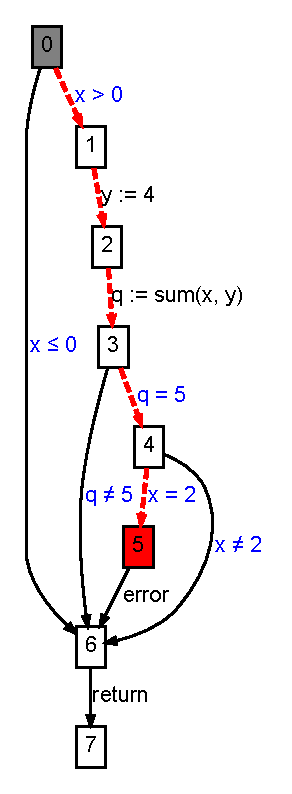
\includegraphics[scale=0.6]{{figs/dashCallcallAddPassExample/4test.graph.0.path}.eps}
		\label{fig:dashCall:findAbstractErrorPath:test}
	}
	\hfil
	\begingroup
	\captionsetup[subfigure]{width=3.5cm}
	\subfloat[Path does not include the \code{sum} procedure]
	{
		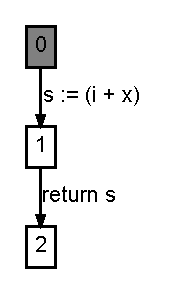
\includegraphics[scale=0.8]{{figs/dashCallcallAddPassExample/2sum.graph}.eps}
		\label{fig:dashCall:findAbstractErrorPath:sum}
	}
	\endgroup
	\caption
	{
		\protect\subref{fig:dashCall:findAbstractErrorPath:test} shows the path found by \classname{FindAbstractErrorPath} for the first iteration of \DASHcall while analyzing the code shown in \cref{fig:dashCall:extendFrontier:inputConstraints}. Notice that the path does not pass through \protect\subref{fig:dashCall:findAbstractErrorPath:sum}.
	}
	\label{fig:dashCall:findAbstractErrorPath}
\end{figure}

% % % % % % % % % % % % % % % % % % % % % % % % % % % % % % % % % % % % % % % % % %
\section{\classname{ConvertToRegionTraceWithAbstractFrontier}}
\label{sec:dashCall:convertToRegionTrace}
The \classname{ConvertToRegionTraceWithAbstractFrontier} procedure needs to be slightly changed. It will construct the trace in the exact same manner as in \DASHint, however, it will also include the states for the part of the trace that follows a concrete execution.

Formally the trace will now have the form $\tau_c = \langle RS_0, \ldots RS_{k-1}, S_k \rangle$ where each $RS_i = \langle S_i, s_i \rangle$ is called a \classname{RegionState}. Each \classname{RegionState} includes the region $S_i$ and the state $s_i$ that was found by following the parent relationship from $s_{k-1}$. The reason that $S_k$ does not include a state is that it is the region after the frontier and therefore no concrete execution has reached it yet.

The states are used in \classname{ExecuteSymbolic} to figure out how to symbolically execute a procedure call edge when these are encountered in a trace. States $s_i$ are thus only needed when the following statement is a procedure call. This is described in \cref{sec:dashCall:executeSubProcedure}, which describes the \classname{ExecuteSymbolic} procedure for \DASHcall.

\cref{fig:dashCall:convert:path} shows a path that is to be converted to a trace. The trace found is shown in \cref{fig:dashCall:convert:trace}. Region 2 includes a state which is prefixed with $\#2$ and region 3 has a state with the prefix $\#6$. These numbers tells us that 3 regions were visited between these two states, and these are recorded on the graph of the sub procedure seen in \cref{fig:dashCall:convert:subproc}. It should be noted that states are only linked inside a single procedure. Thus \classname{Parent}$(\#6)=\#2$ and not $\#5$ as could have been expected.

Writing out the resulting trace in full, including each of the states, produces the following:
\begin{align*}
\tau_c = \langle
 &\langle 0, \#0[y \mapsto 0, x \mapsto 1] \rangle, \\
 &\langle 1, \#1[y \mapsto 0, x \mapsto 1] \rangle, \\
 &\langle 2, \#2[y \mapsto 4, x \mapsto 1] \rangle, \\
 &\langle 3, \#6[q \mapsto 5, y \mapsto 4, x \mapsto 1] \rangle, \\
 &\langle 4, \#7[q \mapsto 5, y \mapsto 4, x \mapsto 1] \rangle, \\
 &~ 5 \rangle
\end{align*}


\begin{figure}
\def \scale {0.6}
	\centering
	\subfloat[Error path found in the \code{test} procedure]
	{
		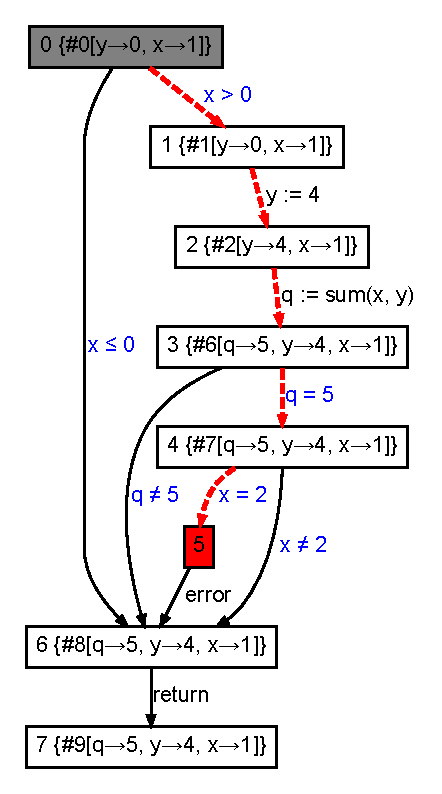
\includegraphics[scale=\scale]{{figs/dashCallcallAddPassExample/7test.graph.1.path}.eps}
		\label{fig:dashCall:convert:path}
	}
	\hfil
	\subfloat[States in the \code{sum} sub procedure]
	{
		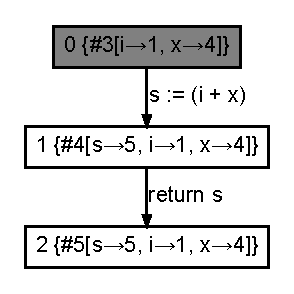
\includegraphics[scale=\scale]{{figs/dashCallcallAddPassExample/4sum.graph.0.autostates}.eps}
		\label{fig:dashCall:convert:subproc}
	}
	\hfil
	\subfloat[Trace found for the path in \protect\subref{fig:dashCall:convert:path}]
	{
		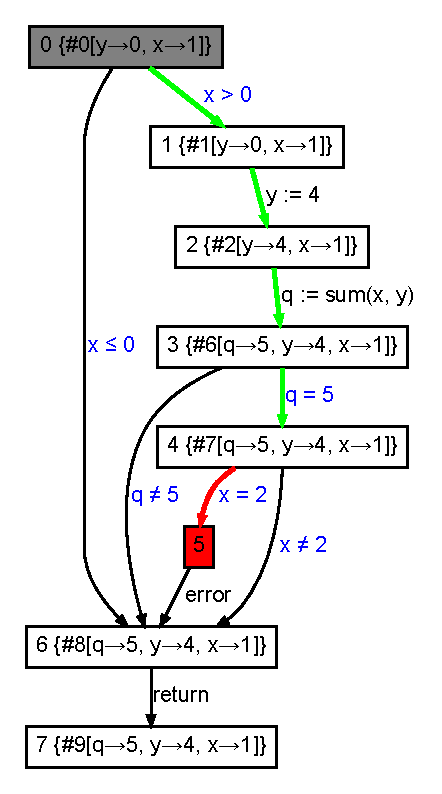
\includegraphics[scale=\scale]{{figs/dashCallcallAddPassExample/8test.graph.1.trace}.eps}
		\label{fig:dashCall:convert:trace}
	}
	\caption
	{
		\classname{ConvertToRegionTraceWithAbstractFrontier} converts the path in \protect\subref{fig:dashCall:convert:path} to the trace in \protect\subref{fig:dashCall:convert:trace}. \protect\subref{fig:dashCall:convert:subproc} shows the states that were added to the \code{sum} procedure when \code{test} procedure was executed by an earlier invocation of \classname{RunTest}. These states are not included in either the path or the trace.
	}
	\label{fig:dashCall:convert}
\end{figure}

The next section presents \classname{ExecuteSymbolic}, the procedure that symbolically executes traces.

\section{\classname{ExecuteSymbolic}}
\label{sec:dashCall:executeSymbolic}
The goal of \classname{ExecuteSymbolic} is to execute a trace $\tau_c$ that traverses the procedure $P$. Compared to \DASHint the new requirements are that \classname{ExecuteSymbolic} handles procedure calls during the trace and additionally returns the symbolic map $\mathpzc{S}$ as it was before executing the frontier statement. As a special case, when the frontier edge is a procedure call, \classname{ExecuteSymbolic} ignores it and leaves it to be handled by \classname{ExtendFrontier}, which is described in \cref{sec:dashCall:extendFrontier}.

\classname{ExecuteSymbolic} has been split into two parts. The \classname{ExecuteSymbolic} algorithm, shown in \cref{alg:dashCall:executeSymbolic}, that executes the trace $\tau_c$, and \classname{ExecuteSymbolicSubProcedure}, shown in \cref{alg:dashCall:executeSubProcedure}, that symbolically executes sub procedures.

\begin{thesisalgorithm}
\caption{\classname{ExecuteSymbolic}($\tau_c=\langle RS_0,\ldots, RS_{k-1},S_{k} \rangle, P, \mathpzc{P}, \mathpzc{G}$)}
\label{alg:dashCall:executeSymbolic}
Returns: $\langle \phi, \mathpzc{S} \rangle$, the path constraint $\phi$ for reaching and crossing the frontier; and the symbolic map $\mathpzc{S}$, from before the frontier.

\begin{algorithmic}[1]
	\State \Let $\langle S_{0}, \_ \rangle = RS_{0}$
	\State \Let $\langle \rho_0, \_ \rangle = S_{0}$
	\State $\mathpzc{S}:= [v \mapsto v_0 \mid v \in \classname{params}(P)]$
	\State $\phi := \classname{SymbolicEval}(\rho_0, \mathpzc{S})$
	
	\\
	\For{$i = 0$ \textbf{to} $k - 2$}
		\State \Let $\langle \_, s_{i} \rangle = RS_{i}$
		\State \Let $\langle S_{i+1}, \_ \rangle = RS_{i+1}$
		\State \Let $\langle \rho_{i+1}, \_ \rangle = S_{i+1}$
		\State $op := \classname{Op}(S_i, S_{i + 1})$
		\Match{$op$}
			\Case{\code{v := e}}
				\State $\mathpzc{S} := \mathpzc{S}[\code{v} \mapsto \classname{SymbolicEval}(\code{e}, \mathpzc{S})]$
			\EndCase
			\Case{\code{assume c}}
				\State $\phi := \phi \wedge\classname{SymbolicEval}(\code{c},\mathpzc{S})$
			\EndCase
			\Case{\code{v := f}$(a_0,\ldots,a_n)$}
				\State $P' := \classname{LookupProcedure}($\code{f}$, \mathpzc{P}$)
				\State $args := \langle \classname{SymbolicEval}(a_i, \mathpzc{S}) \mid \forall a_i \rangle$
				\State $\langle \phi', e' \rangle := \classname{ExecuteSymbolicSubProcedure}(P', args, s_i, \mathpzc{P}, \mathpzc{G})]$
				\State $\phi := \phi \wedge \phi'$ 
				\State $\mathpzc{S} := \mathpzc{S}[\code{v}  \mapsto e']$
			\EndCase
			\Case{\code{return e}}
				\State \Skip
			\EndCase
		\EndMatch
		\State $\phi := \phi \wedge \classname{SymbolicEval}(\rho_{i+1}, \mathpzc{S})$
	\EndFor
	
	\\
	\State \Let $\langle S_{k-1}, \_ \rangle = RS_{k-1}$
	\State \Let $\langle \rho_{k}, \_ \rangle = S_{k}$
	\State $op := \classname{Op}(S_{k-1}, S_{k})$
	\Match{$op$}
		\Case{\code{v := e}}
			\State $\mathpzc{S}' := \mathpzc{S}[\code{v} \mapsto \classname{SymbolicEval}(\code{e}, \mathpzc{S})]$
			\State $\phi := \phi \wedge \classname{SymbolicEval}(\rho_{k}, \mathpzc{S}')$
		\EndCase
		\Case{\code{assume c}}
			\State $\phi := \phi \wedge \classname{SymbolicEval}(\code{c},\mathpzc{S})$
			\State $\phi := \phi \wedge \classname{SymbolicEval}(\rho_{k}, \mathpzc{S})$
		\EndCase
		\Case{\code{v := f}$(a_0,\ldots,a_n)$}
			\State \Skip
		\EndCase
		\Case{\code{return e}}
			\State $\phi := \phi \wedge \classname{SymbolicEval}(\rho_{k}, \mathpzc{S})$
		\EndCase
	\EndMatch
	
	\State \Return $\langle \phi, \mathpzc{S} \rangle$	
\end{algorithmic}
\end{thesisalgorithm}

\classname{ExecuteSymbolic} takes as input a trace $\tau_c$, the procedure $P$, which the trace runs through, the program $\mathpzc{P}$ that contains all the procedures, and finally \classname{ExecuteSymbolic} takes the complete set of graphs $\mathpzc{G}$. As mentioned in \cref{sec:dashCall:convertToRegionTrace} the trace $\tau_c$ has been changed from a trace of regions $\langle S_0, \ldots, S_k \rangle$ to a trace of \classname{RegionState}s $\langle RS_0, \ldots, RS_{k-1}, S_k \rangle$.

To support the added requirements three major changes have been made to the pseudocode of \classname{ExecuteSymbolic}:
\begin{itemize}
	\item The \classname{ExecuteSymbolic} return statement has been changed, such that it also returns the symbolic map $\mathpzc{S}$ before executing the frontier.

	\item Two new cases has been added. These cases handle procedure calls of the form \code{v := f}$(a_0,\ldots,a_n)$ and \code{return e} statements.

	\item To return the symbolic map $\mathpzc{S}$ as it is seen before the frontier is executed, and because procedure calls are handled differently if they are included before the frontier edge, the execution of the frontier edge has been unrolled from the loop.
\end{itemize}

\classname{ExecuteSymbolic} returns the same path constraint $\phi$ that would be found by the \DASHint version of \classname{ExecuteSymbolic}, when executing a trace that does not include a procedure call. However, \classname{ExecuteSymbolic} for \DASHcall also returns the symbolic map $\mathpzc{S}$.

\subsubsection{Execution of the trace before the frontier}
The loop in \cref{alg:dashCall:executeSymbolic} behaves the same as in \DASHint except that it does not execute the frontier statement, and it additionally handles procedure calls. Edges with \code{return e} statements can never occur before the frontier edge in a trace $\tau_c$. This is because there are no outgoing edges from regions with incoming \code{return} edges, since execution stops when a \code{return} statement is executed. The \code{return e} case in lines 22-23 has been included in the pseudocode for completeness, but will never be triggered and thus it is simply skipped.

Since procedures only see their parameters and cannot alter global state, handling them symbolically is a matter of constructing the correct parameters for them. Lines 16-21 handles procedure calls of the form \code{v := f}$(a_0,\ldots,a_n)$. The arguments $a_0,\ldots,a_n$ to the procedure call are each symbolically evaluated and added to a list $args$ in line 18, which functions as the symbolic values of the parameters. Thus if a procedure takes as input $x$, then the symbolic expression of $x$, which could be $x_0+y_0/3$, will be in $args$. The symbolic expressions consist of expressions including only constants or the initial symbolic values generated in line 3.

A call is made to \classname{ExecuteSymbolicSubProcedure} in line 19, which is responsible for executing the sub procedure symbolically. It is important that \classname{ExecuteSymbolicSubProcedure} follows the same execution that was followed in the trace $\tau_c$. Therefore, it is among others given the state $s_i$ from the trace $\tau_c$, which is the state that existed prior to executing the procedure call. The region graph for the called procedure $P'$ might contain many concrete executions from prior invocations of \classname{RunTest} and \classname{ExecuteSymbolicSubProcedure} uses $s_i$ to find the concrete execution that was generated by the execution that $\tau_c$ follows.

The call to \classname{ExecuteSymbolicSubProcedure} returns an induced path constraint $\phi'$ from the procedure call and the symbolic expression $e'$ that represents the computation performed by the called procedure. The path constraint $\phi'$ is added to $\phi$ in line 20 while \code{v} is assigned the symbolic return value $e'$ in line 21. Execution of sub procedures, which is performed by \classname{ExecuteSymbolicSubProcedure}, is described in \cref{sec:dashCall:executeSubProcedure}.

\subsubsection{Execution of the frontier}
There are multiple changes to how the frontier statement is being symbolically executed. We need to return the symbolic map $\mathpzc{S}$ as it was before executing the frontier statement. This is a requirement enforced by \classname{ExtendFrontier}, which uses it when handling procedure calls at the frontier edge. \classname{ExecuteSymbolic} still needs to handle assignments and \code{assume c} statements, but it also needs to handle \code{return e} statements as part of the frontier.

If the frontier statement is a procedure call \code{v := f}$(a_0,\ldots,a_n)$ then \classname{ExecuteSymbolic} skips it in lines 37-38. Procedure calls at the frontier will be handled by \classname{ExtendFrontier} described in \cref{sec:dashCall:extendFrontier}. The reason is that \classname{ExecuteSymbolic} does not have a trace that it can follow in the called procedure, and it therefore has a large number of possible execution paths that it could select for symbolic execution in the called procedure. Choosing one path might make the combined path constraint feasible while choosing another path might make it infeasible.

In essence the question given is a reachability question: Can a path be found in the procedure \code{f}, under the symbolic state $\mathpzc{S}$ and with the path constraint $\phi$, such that a state $s$ is generated that satisfies the region predicate after the frontier. This is exactly the kind of questions that \DASH is constructed to answer and \classname{ExtendFrontier} exploits this, as we shall see in \cref{sec:dashCall:extendFrontier}. Thus \classname{ExecuteSymbolic} skips procedure calls at the frontier edge and leaves the work to be completed by \classname{ExtendFrontier}.

What is left to be handled are \code{assume c}, assignments and \code{return e} statements. Symbolically executing the region predicate has been moved into each of the cases since the case that handles procedure calls does not symbolically execute the region predicate. All \code{assume c} statements are handled exactly as if they had occurred before the frontier.

Assignments are handled in lines 31-33. The assignment operation needs special handling since it changes the state of the symbolic map. This state change is needed when evaluating the region after the frontier. However we need to return the state of the symbolic map before the frontier. The temporary symbolic map $\mathpzc{S'}$ is therefore introduced and holds the symbolic map $\mathpzc{S}$ with state applied by the assignment, and it is then used when evaluating the region predicate after the frontier. The symbolic map $\mathpzc{S}$ remains unchanged.

The last kind of statements that can occur is the \code{return e} statement. The \code{return e} statement does not change the symbolic state, nor the path constraint, therefore only the region predicate needs to be symbolically executed, which is completed in line 40.

The next section describes \classname{ExecuteSymbolicSubProcedure}, which executes called sub procedures during the trace $\tau_c$.

\subsection{\classname{ExecuteSymbolicSubProcedure}}
\label{sec:dashCall:executeSubProcedure}
The pseudocode for \classname{ExecuteSymbolicSubProcedure} is shown in \cref{alg:dashCall:executeSubProcedure}. The goal of this procedure is to symbolically execute a called sub procedure. It returns the generated path constraint $\phi$ and the symbolic return value $e$. The following input is given to \classname{ExecuteSymbolicSubProcedure}: 

\begin{itemize}
	\item The called procedure $P$, which should be symbolically executed.
	
	\item The symbolically evaluated arguments in $args$, which represents the parameters of $P$ in terms of the initial symbolic variables generated in \classname{ExecuteSymbolic}.
	
	\item The state $s_{caller}$ before the procedure call that is used to find the concrete execution to follow in $P$.
	
	\item Additionally \classname{ExecuteSymbolicSubProcedure} is given the program $\mathpzc{P}$ and the set of graphs $\mathpzc{G}$, which are used for looking up procedures and graphs.
\end{itemize}

\begin{thesisalgorithm}
\caption{\classname{ExecuteSymbolicSubProcedure}($P, args = \langle b_0, \ldots, b_{n} \rangle, s_{caller}, \mathpzc{P}, \mathpzc{G}$)}
\label{alg:dashCall:executeSubProcedure}
Returns: $\langle \phi, e \rangle$, $\phi$ is the induced path constraint and $e$ is the symbolic return value of the procedure invocation.

\begin{algorithmic}[1]
	\State $\mathpzc{S} := [v_i \mapsto b_i \mid \forall v_i \in \classname{params}(P)$]
	\State $G := \classname{LookupRegionGraph}(P, \mathpzc{G})$
	\State $S_{prev} :=  \classname{InitialRegion}(G)$
	\State $s_{prev} := \classname{FindCalleeStateFromCallersState}(s_{caller}, S_{prev})$
	\State $\phi :=$ \code{true}
	\\
	
	\Loop
		\State $s_{next} := \classname{Child}(s_{prev})$
		\State $S_{next} := \classname{FindRegionWithState}(\classname{Children}(S_{prev}), s_{next})$

		\State $op := \classname{Op}(S_{prev}, S_{next})$
		\Match{$op$}
			\Case{\code{v := e}}
				\State $\mathpzc{S} := \mathpzc{S}[\code{v} \mapsto \classname{SymbolicEval}(\code{e}, \mathpzc{S})]$
			\EndCase
			\Case{\code{assume c}}
				\State $\phi := \phi \wedge \classname{SymbolicEval}(\code{c},\mathpzc{S})$
			\EndCase
			\Case{\code{v := f}$(a_0,\ldots,a_n)$}
				\State $P' := \classname{LookupProcedure}($\code{f}$, \mathpzc{P}$)
				\State $args' := \langle \classname{SymbolicEval}(a_i, \mathpzc{S}) \mid \forall a_i \rangle$
				\State $\langle \phi', e' \rangle := \classname{ExecuteSymbolicSubProcedure}(P', args', s_{prev}, \mathpzc{P}, \mathpzc{G})]$
				\State $\phi := \phi \wedge \phi'$ 
				\State $\mathpzc{S} := \mathpzc{S}[$\code{v} $ \mapsto e']$
			\EndCase
			\Case{\code{return e}}
				\State $e_{result} := \classname{SymbolicEval}(\code{e}, \mathpzc{S})$
				\State \Return $\langle \phi, e_{result} \rangle$
				
			\EndCase
		\EndMatch
		\State $s_{prev} := s_{next}$
		\State $S_{prev} := S_{next}$
	\EndLoop
	
\end{algorithmic}
\end{thesisalgorithm}

\classname{ExecuteSymbolicSubProcedure} functions in nearly the same way as \classname{ExecuteSymbolic}. As in \classname{ExecuteSymbolic} there is a loop that executes the trace, and the cases for assignments, assumes and procedure calls are nearly identical. However, there are some differences:
\begin{itemize}
	\item The initial symbolic variables for the parameters of $P$ is given in $args$. This is shown in line 1 which sets the initial symbolic variables to the ones given in $args$, and thus does not create new symbolic variables $v_0$.
	
	\item In \classname{ExecuteSymbolic} a trace $\tau_c$ is given and followed. In \classname{ExecuteSymbolicSubProcedure} the initial region of the called procedure and the concrete execution to follow needs to be found, this is completed in lines 3-4. Additionally the trace needs to be explicitly maintained, which is fulfilled in lines 8-9 and 25-26.
	
	\item When a \code{return e} statement is encountered it ends the symbolic execution of the sub procedure $P$. \classname{ExecuteSymbolicSubProcedure} then returns the path constraint $\phi$ and the symbolic expression that represents the result of following the induced trace in $P$.
	
	\item Region predicates are not executed since the regions of subgraphs do not contain predicates. Only the graph that \classname{ExecuteSymbolic} works on can be refined, and it is therefore the only graph that can have predicates on the regions.
\end{itemize}

The construction of the initial symbolic map is performed in line 1. This is completed by mapping the formal parameters to their corresponding arguments provided in $args$. This ensures that any symbolically evaluated expressions will only contain expressions with constants or initial symbolic variables $v_0$ generated in \classname{ExecuteSymbolic}.

To start the execution, \classname{ExecuteSymbolicSubProcedure} needs to find the initial state in the concrete execution that it should follow in the sub procedure. The concrete execution that should be followed is the one that was generated by calling $P$ when in the state $s_{caller}$. Finding the initial state is accomplished by first finding the initial region of $P$, in line 3, with a call to \classname{InitialRegion}. \classname{ExecuteSymbolicSubProcedure} then needs to find the state in the initial region that was generated by $s_{caller}$. This is accomplished in line 4 with a call to \classname{FindCalleeStateFromCallersState}. Each of our states contain both a test id, which is unique for each \classname{RunTest} invocation, and it contains the number of steps taken in the execution. Given that $s_{caller}$ has a test id we know that the initial state must have the same test id. Also, if the state $s_{caller}$ has taken $n$ steps in the execution, then the initial state must have taken exactly $n+1$ steps. Given these two pieces of information, we can find the initial state.

The initial region is assigned to $S_{prev}$, while the region that \classname{ExecuteSymbolicSubProcedure} is about to transition to is called $S_{next}$. The same convention is used for the concrete states $s_{prev}$ and $s_{next}$. We use the child relationship on $s_{prev}$ to find $s_{next}$. The region $S_{next}$ that contains $s_{next}$ can be found by going through all the child regions of $S_{prev}$ and find the region that contains $s_{next}$. This is exactly what \classname{FindRegionWithState} does. The regions $S_{prev}$ and $S_{next}$ can then be used to find the operation $op$ to be executed. After executing the operation $op$, $s_{prev}$ and $S_{prev}$ is set to $s_{next}$ and $S_{next}$ to prepare for the next iteration of the loop.

This concludes the explanation of \classname{ExecuteSymbolic} and \classname{ExecuteSymbolicSubProcedure}. In the next section an example of them is given.

\subsection{Example of \classname{ExecuteSymbolic}}
As an example of how \classname{ExecuteSymbolic} functions in \DASHcall, we will symbolically execute the trace found in \cref{fig:dashCall:executesymbolic:caller}.

\begin{figure}
\def \scale {0.6}
	\centering
	\subfloat[The main procedure \code{test}]
	{
		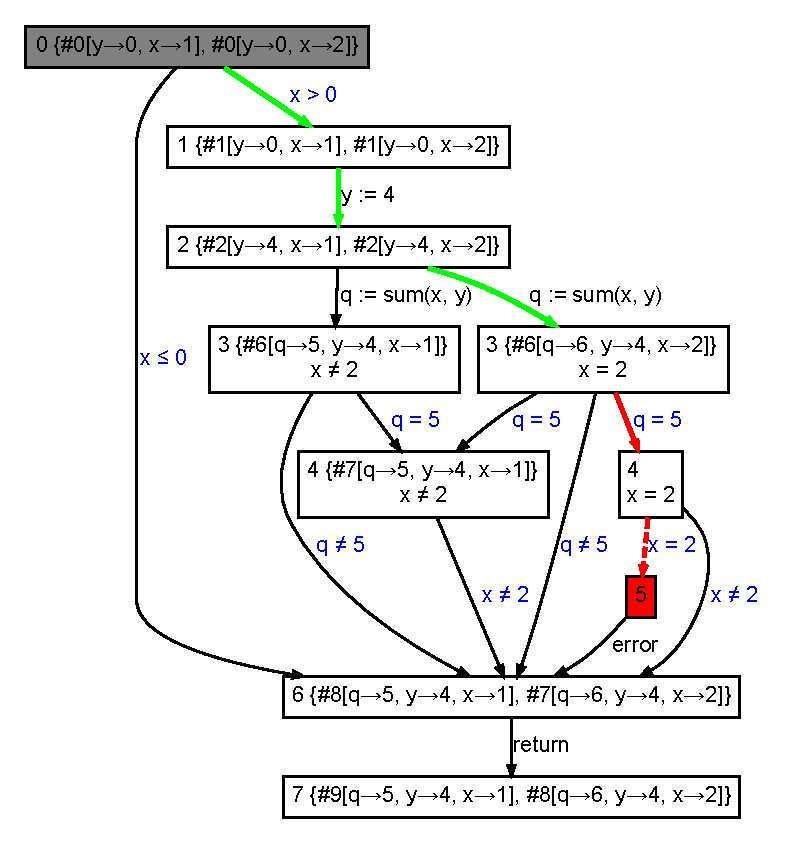
\includegraphics[scale=\scale]{{figs/dashCallcallAddPassExample/24test.graph.4.trace}.eps}
		\label{fig:dashCall:executesymbolic:caller}
	}
	\hfil
	\subfloat[The called procedure \code{sum}]
	{
		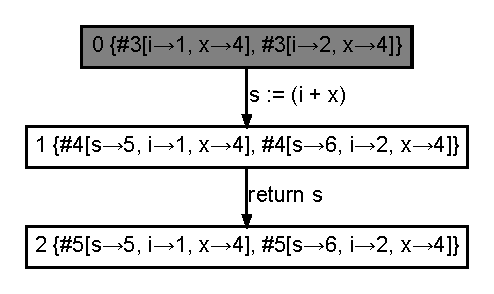
\includegraphics[scale=\scale]{{figs/dashCallcallAddPassExample/31sum.graph.3.autostates}.eps}
		\label{fig:dashCall:executesymbolic:callee}
	}
	\caption
	{
		\protect\subref{fig:dashCall:executesymbolic:caller} shows a trace that needs to be symbolically executed, which contains a call before the frontier to the sub procedure in \protect\subref{fig:dashCall:executesymbolic:callee}.
	}
	\label{fig:dashCall:executesymbolic}
\end{figure}

In \cref{fig:dashCall:executesymbolic:caller} we can see the trace $\langle 0, 1, 2, 3{:}x{=}2, 4{:}x{=}2 \rangle$ following the green edges down and including the red frontier. The green part of the trace is found by following the concrete states where $x \mapsto 2$, which is included in the trace $\tau_c$.

\subsubsection{Setup and symbolically evaluating the initial region}
At startup the symbolic map $\mathpzc{S}_{test}$ for the \code{test} procedure is set to $[x \mapsto x_0, y \mapsto y_0]$. Symbolically evaluating the region predicate of the initial region sets $\phi_{test}$ to \code{true} resulting in the state of \classname{ExecuteSymbolic} becoming:
\begin{align*}
	\phi_{test} &\is \text{\code{true}}\\
	\mathpzc{S}_{test} &\is [x \mapsto x_0, y \mapsto y_0]
\end{align*}

\subsubsection{Symbolically executing \code{assume} $x > 0$ on edge $(0, 1)$}
There are no changes to how this and the next step is symbolically executed compared to how \DASHint would execute them. The step $(0, 1)$ executes the \code{assume} $x > 0$ statement and symbolically evaluates the region predicate in region 1, which is \code{true}. The \code{assume} $x > 0$ statement adds $x_0 > 0$ to $\phi_{test}$. The symbolic map is left unchanged. The region predicate for region 1 is \code{true} and therefore nothing new was added to $\phi_{test}$ while executing it. After this step the state of \classname{ExecuteSymbolic} is:
\begin{align*}
	\phi_{test} &\is x_0 > 0\\
	\mathpzc{S}_{test} &\is [x \mapsto x_0, y \mapsto y_0]
\end{align*}

\subsubsection{Symbolically executing \code{y := 4} on edge $(1, 2)$}
The second edge $(1, 2)$ with $y := 4$, updates the mapping for $y$ in the symbolic map $\mathpzc{S}_{test}$. Since the region predicate is \code{true} $\phi_{test}$ is not affected. This leads to the \classname{ExecuteSymbolic} state:
\begin{align*}
	\phi_{test} &\is x_0 > 0\\
	\mathpzc{S}_{test} &\is [x \mapsto x_0, y \mapsto 4]
\end{align*}

\subsubsection{Symbolically executing the \code{q := sum(x, y)} call on edge $(2, 3{:}x{=}2)$}
This step symbolically executes the operation \code{q := sum(x, y)}. First we find the procedure description $P_{sum}$ for \code{sum}, in line 17, by a call to \classname{LookupProcedure}. Then the symbolic argument list $args$ is constructed. The variables $x$ and $y$ are used as arguments to \code{sum} and symbolically evaluating them results in $args=\langle x_0, 4 \rangle$.

\classname{ExecuteSymbolicSubProcedure} is called in line 19 which executes the sub procedure. It takes as arguments the called procedure $P_{sum}$, $args$ and additionally the current concrete state, which is $s_2=\#2[y\mapsto4, x\mapsto2]$, the program $\mathpzc{P}$ and all graphs $\mathpzc{G}$.

\subsubsection{Symbolically executing \code{sum(x, y)} with \classname{ExecuteSymbolicSubProcedure}}
\classname{ExecuteSymbolicSubProcedure} starts by setting up its own symbolic map $\mathpzc{S}_{sum}$ from the symbolic argument list $args$, which then becomes $[i \mapsto x_0, x \mapsto 4]$. It then finds the graph $G_{sum}$ for the current procedure $P_{sum}$ such that it can find the initial region and store it in $S_{prev}$. 

The initial region is region 0 in \cref{fig:dashCall:executesymbolic:callee}. We need to find the state that follows the state $s_2$ given as $s_{caller}$. In region 0 there are two states, namely  $\#3[i \mapsto 1, x \mapsto 4]$ and $\#3[i \mapsto 2, x \mapsto 4]$. The states additionally have a test id attached. Both states have the same number of execution steps, namely 3. However, only one state has the same test id as $s_{caller}$ and in this case it is the state $\#3[i\mapsto2, x\mapsto4]$. This state is assigned to the variable $s_{prev}$.

Transitioning between regions in \code{sum} is trivial since there is only a single outgoing edge from each region. However, in the general case, there can multiple outgoing edges because of conditionals, and \classname{ExecuteSymbolicSubProcedure} needs to figure out which edge to follow. This is accomplished by finding the next state $s_{next}$ by following the child relationship on $s_{prev}$. For the first iteration, $s_{next}$ is the state $\#4[s\mapsto6, i\mapsto2, x\mapsto4]$. Using the state $s_{next}$ the region $S_{next}$ is found, which is region 1.

The edge between region 0 and region 1 has the operation $s := (i + x)$ and the symbolic map $\mathpzc{S}_{sum}$ is therefore updated to $[s \mapsto x_0 + 4, i \mapsto x_0, x \mapsto 4]$ and $\phi$ is left unchanged. Afterwards $s_{prev}$ is set to the state $s_{next}=\#4[s\mapsto6, i\mapsto2, x\mapsto4]$ and $S_{prev}$ is set to $S_{next}$, which is region 1.

The next state $s_{next}$ is found, and in this case it is $\#5[s\mapsto6, i\mapsto2, x\mapsto4]$. The region that the state is contained in, region 2, is assigned to $S_{next}$. The operation on the edge $(1, 2)$ is the return statement \code{return} $s$. Symbolically evaluating this yields the result $e_{result}=x_0 + 4$, which is returned from \classname{ExecuteSymbolicSubProcedure} together with the path constraint \code{true}.

\subsubsection{Handling return from the procedure call \code{q := sum(x, y)}}
When \classname{ExecuteSymbolicSubProcedure} returns, \classname{ExecuteSymbolic} stores the path constraint in $\phi'$ and the result in $e'$. The path constraint is added to $\phi$, but since $\phi'$ is \code{true} then $\phi$ is left unchanged. The assigned variable $q$ is updated to the value $e'$ in the symbolic map $\mathpzc{S}_{test}$, such that it maps to the symbolic expression $x_0 + 4$ returned by \classname{ExecuteSymbolicSubProcedure}. Finally, the region predicate from region 3, which is $x = 2$, is symbolically evaluated and added to $\phi$ resulting in the state of \classname{ExecuteSymbolic} becoming:
\begin{align*}
	\phi_{test} &\is x_0 > 0 \wedge x_0 = 2\\
	\mathpzc{S}_{test} &\is [x \mapsto x_0, y \mapsto 4, q \mapsto x_0 + 4]
\end{align*}

\subsubsection{Symbolically executing \code{assume} $q=5$ at the frontier edge $(3{:}x{=}2, 4{:}x{=}2)$}
\classname{ExecuteSymbolic} exits the loop, since it is about to execute the frontier edge $(3{:}x{=}2, 4{:}x{=}2)$. This edge has the operation \code{assume} $q=5$ and the region after it contains the predicate $x=2$. Evaluating both of these predicates, adding them to $\phi$, and removing duplicate terms results in the path constraint $\phi = x_0 > 0 \wedge x_0 = 2 \wedge x_0 + 4 = 5$. The result returned from \classname{ExecuteSymbolic} is thus:
\begin{align*}
	\phi &\is x_0 > 0 \wedge x_0 = 2 \wedge x_0 + 4 = 5\\
	\mathpzc{S} &\is [x \mapsto x_0, y \mapsto 4, q \mapsto x_0 + 4]
\end{align*}

This path constraint will be found unsatisfiable by \classname{ExtendFrontier}, due to the constraints $x_0 = 2 \wedge x_0 + 4 = 5$.

The next section explains \classname{ExtendFrontier} and how procedure calls are handled when they are encountered at the frontier edge.

\section{\classname{ExtendFrontier}}
\label{sec:dashCall:extendFrontier}
\classname{ExtendFrontier} for \DASHcall behaves the same as in \DASHint for all traces except when the frontier is a procedure call. In this case, \classname{ExtendFrontier} performs additional work that requires extra information passed from \classname{DashLoop}. As in \DASHint, \classname{ExtendFrontier} takes the trace $\tau_c$ and the procedure currently being analyzed $P$. Additionally, it takes the region graphs for all procedures $\mathpzc{G}$ and the full program $\mathpzc{P}$ as arguments. The \DASHcall variant of \classname{ExtendFrontier} is shown in \cref{alg:dashCall:extendFrontier}.

\begin{thesisalgorithm}
\caption{\classname{ExtendFrontier}($\tau_c = \langle RS_0, \ldots, RS_{k-1}, S_k \rangle, P, \mathpzc{G}, \mathpzc{P}$)}
\label{alg:dashCall:extendFrontier}
Returns:\\
$\langle t,$ \code{true}$ \rangle$, if the frontier can be extended; or\\
$\langle \unsat, \rho \rangle$, if the frontier cannot be extended

\begin{algorithmic}[1]
	\State \Let $\langle S_{k-1}, \_ \rangle = RS_{k-1}$
	\State $\langle \phi, \mathpzc{S} \rangle := \classname{ExecuteSymbolic}(\tau_c, P, \mathpzc{P}, \mathpzc{G}$)
	\State $op := \classname{Op}(S_{k-1}, S_k)$
	\If{$op$ \matches $\code{v := f}(a_0,\ldots,a_n)$}
		\State \Let $\langle \rho_k, \_ \rangle = S_{k}$
		\State $P' := \classname{Lookup}(\code{f}, \mathpzc{P})$
		\State $\pi := \classname{CreateVariableRenamer}(\classname{locals}(P) \cup \{v, v_0 \mid \forall v \in \classname{params}(P)\})$
		\State $\phi_{ic} := \Big( \bigwedge_{v_i \in \classname{params}(P')} v_i = \pi(a_i) \Big)
				    \wedge \Big( \bigwedge_{(w \mapsto e) \in \mathpzc{S}} \pi(w = e) \Big) \wedge
				    \pi(\phi) $
		\State $\phi_{ec} := \pi(\rho_k[@r/\code{v}])$
		\State $\mathpzc{G}' := \classname{ReconstructGraphsAndInsertConstraints}(\mathpzc{G}, \phi_{ic}, \phi_{ec}, P')$
		\State $\langle r, z \rangle = \classname{DashLoop}(\mathpzc{G}', \mathpzc{P}, P')$
		\If {$r = \fail$}
			\State $t := \pi^{-1}\Big(z \setminus \{v_0 \mid \forall v \in \classname{params}(P')\} \Big) \setminus \Big(\classname{locals}(P) \cup \classname{params}(P)\Big)$
			\State $\rho :=$ \code{true}
		\Else
			\State $t := \unsat$
			\State $\rho := \pi^{-1}
							\left(
								\left(
									\bigvee_{\rho_i \in \classname{InitialRefines}(z)}\rho_i
								\right)
								\big[a_0/v_0, \ldots, a_n/v_n\big]~\mid v_i \in \classname{params}(P')
							\right)$
		\EndIf
	\Else
		\State $t := \classname{IsSAT}(\phi, P)$
		\If{$t = \unsat$}
			\State $\rho := \classname{RefinePred}(\tau_c)$
		\Else
			\State $\rho :=$ \code{true}
		\EndIf
	\EndIf
	\State \Return $\langle t, \rho \rangle$
\end{algorithmic}
\end{thesisalgorithm}

If the frontier edge $(S_{k-1}, S_k)$ is a procedure call \code{v := f}$(a_0, \ldots, a_n)$, then the job of \classname{ExtendFrontier} is to check if it is possible to reach a state $s$ by calling \code{f} such that the state $s$ satisfies the region predicate from $S_k$. By encoding this problem on the called procedure $P'$ in a clever way, we can use \classname{DashLoop} to answer the problem. We wish to invoke \classname{DashLoop} on the called procedure $P'$ such that:

\begin{itemize}
	\item If \classname{DashLoop} reports that an error could be reached with test input $t$, then we are able to run a test that crosses the frontier procedure call and get a state $s$ that satisfies the region predicate in $S_k$.

	\item If \classname{DashLoop} reports that no errors could be reached with a graph $G$ as proof, then a refinement predicate $\rho$, which eliminates the trace $\tau_c$ in the caller procedure, can be obtained by inspecting the proof $G$.
\end{itemize}

This can be achieved by running \classname{DashLoop} on a slightly altered version of $P's$ region graph. The job of \classname{ExtendFrontier} is now to:

\begin{itemize}
	\item Compute the input constraint $\phi_{ic}$ for the analysis of $P'$, such that only values that can be generated by following the trace $\tau_c$ in $P$ can be used when analyzing $P'$.
	
	\item Encode the region predicate of $S_k$ into an exit constraint $\phi_{ec}$ such that if analysis of $P'$ reaches a region with $\phi_{ec}$, then $S_k$ can be reached in the caller procedure $P$.
	
	\item Use $\phi_{ic}$ and $\phi_{ec}$ to alter $P'$s initial region graph $G'$.
	
	\item Invoke \classname{DashLoop} on the altered region graph $G'$.
	
	\item When \classname{DashLoop} returns, either extract the test input needed to call procedure $P$ such that the frontier is crossed, or construct a refinement predicate to refine the region graph $G$, making $\tau_c$ infeasible in $P$.
\end{itemize}

Furthermore, \classname{ExtendFrontier} has to rename variables in the constraints $\phi_{ic}$ and $\phi_{ec}$, otherwise these variables might clash with variables in the called procedure.

The first lines of \classname{ExtendFrontier}, shown in \cref{alg:dashCall:extendFrontier}, should be familiar. \classname{ExecuteSymbolic} is called in line 2, returning a path constraint $\phi$ and the symbolic map $\mathpzc{S}$ that existed before the frontier. Line 4 checks if the operation performed on the frontier edge is a procedure call. If it is not, \classname{ExtendFrontier} behaves exactly like in \DASHint. 

If the operation is a procedure call \code{v := f}$(a_0,\ldots,a_n)$ then \classname{ExecuteSymbolic} did not symbolically execute it, and it is then the job of \classname{ExtendFrontier} to check if the frontier edge can be crossed. In line 6, \classname{ExtendFrontier} starts by looking up the called procedure \code{f} in the program $\mathpzc{P}$, and finds the procedure $P'$. The next lines of \classname{ExtendFrontier} construct the input and exit constraints, invokes \classname{DashLoop}, and extracts the result of \classname{DashLoop}. The next sections describe how each of these tasks is fulfilled by \classname{ExtendFrontier}.

\subsection{Renaming}
In line 7, a variable renamer $\pi$ is constructed by giving it a set of variables that it should rename, while any other variable should be left unchanged. The variables that needs to be renamed are all those variables that originate from the callers procedure $P$, such that they do not conflict with any variables in the callee's procedure $P'$. These are the local variables of $P$, parameters of $P$ and the initial symbolic values $v_0$ generated in \classname{ExecuteSymbolic} for the parameters of $P$. As an example, lets say that $\classname{locals}(P)=\{x,y\}$ and $\classname{params}(P)=\{a,b,c\}$. The construction of the renamer, in line 7, then proceeds as:
\begin{alignat*}{3}
\pi &~~:=&& \classname{CreateVariableRenamer}(\classname{locals}(P) \cup \{v, v_0 \mid \forall v \in \classname{params}(P)\})\\
	&\is&&    \classname{CreateVariableRenamer}(\{x,y\} \cup \{v, v_0 \mid \forall v \in \{a,b,c\}\})\\
	&\is&&    \classname{CreateVariableRenamer}(\{x,y\} \cup \{a, a_0, b, b_0, c, c_0\})\\
	&\is&&    \classname{CreateVariableRenamer}(\{x,y, a, a_0, b, b_0, c, c_0\})
\end{alignat*}

Thus the variables $\{x,y, a, a_0, b, b_0, c, c_0\}$ should be renamed. This also illustrates that the notation $\{v, v_0 \mid \forall v \in \classname{params}(P)\}$ is a set that includes the parameters and their initial symbolic variables that were generated by \classname{ExecuteSymbolic}.

The renamer uses a unique number and a character '$\rename$', which is not allowed in the source code, to rename variables. As such, $\pi(a)$ becomes $1\rename a$ if $a$ is a variable that should be renamed and $1$ is the unique number chosen when $\pi$ was constructed. Whenever the symbol '$\rename$' is seen on a variable in a region graph, it is evident that the variable is external to the procedure. The operation $\pi^{-1}$ is used to reverse the renaming and as such $\pi^{-1}(1\rename a)$ becomes the original variable $a$.

Alternatively we could have created a renamer that renames all occurrences of variables by prepending it with '$\rename$' such that $\pi(a)$ becomes $\rename a$ and $\pi(\rename a)$ becomes $\rename\rename a$. When reverse renaming, the expression $\pi(\rename\rename a)$ becomes $\rename a$ and variables that have not been renamed, such as $a$ are not reverse renamed. The reason why our pseudocode explicitly lists the variables that should be renamed are twofold: 1) because it seems cleaner to explicitly rename only those variables that absolutely needs to be renamed and 2) because our implementation uses \Zthree to perform the renaming that requires us to list the individual variables and their renamed counterparts. The variables that we do not rename, are those that have been renamed once before.

\subsection{Constructing the input constraint $\phi_{ic}$}
\label{sec:dashCall:extendFrontier:inputconstraint}
The input to the called procedure $P'$ must be restricted, such that only test input that is possible by following the trace $\tau_c$ in the caller procedure $P$, is allowed. How this is accomplished is described in this section.

For example, the code for the procedure \code{test} shown in \cref{fig:dashCall:extendFrontier:inputConstraints:caller} calls the \code{sum} procedure shown in \cref{fig:dashCall:extendFrontier:inputConstraints:callee}. The call made to \code{sum} is made with the actual arguments $x$ and $y$, and \code{sum} takes the formal parameters $i$ and $x$. Since both procedures use $x$ as variables, these will be disambiguated with $x_{test}$ and $x_{sum}$ in this presentation. Both of the variables $x_{test}$ and $y$ are constrained in \code{test} at the point where \code{sum} is called. The variable $x_{test}$ must be positive and $y$ must be equal to 4. The analysis of the \code{sum} procedure must similarly constrain the variables $i$ and $x_{sum}$. Since $x_{test}$ is given as $i$ then $i$ must be positive and since $y$ is given for $x_{sum}$ then $x_{sum}$ must be 4.

In general, there are two possible origins of constraints. One origin is the path constraint $\phi$ generated by \classname{ExecuteSymbolic}. In the example $x_{test}$ is used for the parameter $i$, and since the symbolic value $x_{test}$ is constrained to only positive values in the path constraint $\phi$, then $i$ must also be constrained to positive values. The second origin for constraints is the symbolic map $\mathpzc{S}$. In the example $y$ is set to the constant $4$ prior to the \code{sum} procedure call. Since $y$ is passed for the variable $x_{sum}$, then $x_{sum}$ must be equal to $4$. This constraint is not captured by the path constraint $\phi$, but it is captured by the symbolic map, which at this point contains the mapping $y \mapsto 4$.

Furthermore the exit constraint $\phi_{ec}$, constructed in the next section, may contain predicates which use local variables of the caller procedure, but where those variables are not passed as inputs to the callee. The constraints on these variables must also be added to the input constraint such that $\phi_{ec}$ is correctly bound to them. Thus, the input constraint constructed in line 8 uses the formula:
\begin{align*}
\phi_{ic} :=& \left( \bigwedge_{v_i \in \classname{params}(P')} v_i = \pi(a_i) \right) \wedge
            \left( \bigwedge_{(w \mapsto e) \in \mathpzc{S}} \pi(w = e) \right) \wedge
		    \pi(\phi) 
\end{align*}

First, the formal parameters are bound to the actual arguments. Second, the symbolic map $\mathpzc{S}$ is added where each mapping is seen as an equality predicate and finally the path constraint $\phi$ is appended. Renaming is used on all the constraints except on the formal parameters of the called procedure $P'$.

\subsubsection{Example of computing the input constraint}
This section presents an example of computing the input constraint. \Cref{fig:dashCall:extendFrontier:inputConstraints:graph:caller} shows the region graph for the \code{test} procedure listed in \cref{fig:dashCall:extendFrontier:inputConstraints:caller}, after a number of iterations have been performed by \DASHcall. The trace $\tau_c$ shown in the region graph has a frontier edge that is a procedure call to \code{sum}. \classname{ExtendFrontier} constructs the region graph shown in \cref{fig:dashCall:extendFrontier:inputConstraints:graph:callee} and invokes \classname{DashLoop} on it. 

\begin{figure}
\def \scale {0.70}
	\centering
	\subfloat[Region graph for the \code{test} procedure]
	{
		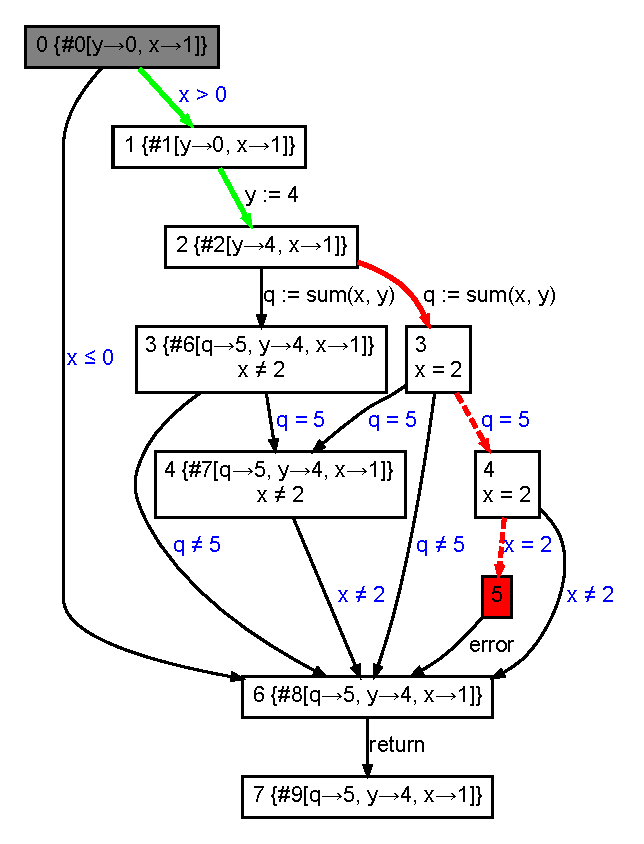
\includegraphics[scale=\scale]{{figs/dashCallcallAddPassExample/14test.graph.3.trace}.eps}
		\label{fig:dashCall:extendFrontier:inputConstraints:graph:caller}
	}
	\hfill
	\subfloat[Intial region graph for \code{sum}]
	{
		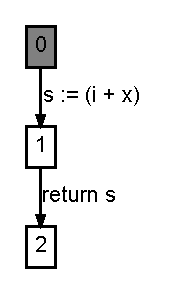
\includegraphics[scale=\scale]{{figs/dashCallcallAddPassExample/2sum.graph}.eps}
		\label{fig:dashCall:extendFrontier:inputConstraints:graph:calleeInitial}
	}
	\hfill
	\subfloat[Region graph with input and exit constraints for \code{sum}]
	{
		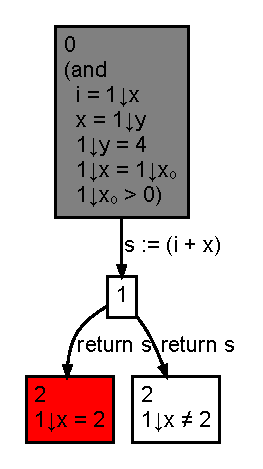
\includegraphics[scale=\scale]{{figs/dashCallcallAddPassExample/15sum.graph.0.init}.eps}
		\label{fig:dashCall:extendFrontier:inputConstraints:graph:callee}
	}
	\caption
	{
		\protect\subref{fig:dashCall:extendFrontier:inputConstraints:graph:caller} shows a region graph for the \code{test} procedure after a number of iterations of \DASHcall. The current frontier is a procedure call to \code{sum}. The initial region graph for \code{sum} is shown in \protect\subref{fig:dashCall:extendFrontier:inputConstraints:graph:calleeInitial} and the graph generated by \classname{ExtendFrontier} for the call to \code{sum} is shown in \protect\subref{fig:dashCall:extendFrontier:inputConstraints:graph:callee}.
	}
	\label{fig:dashCall:extendFrontier:inputConstraints:graph}
\end{figure}

The initial region for \code{sum} in \cref{fig:dashCall:extendFrontier:inputConstraints:graph:callee} shows the added input constraint. First the formal parameters are bound to the actual arguments from \code{test}. In this case, $x_{test}$ is bound to $i$ and $y$ is bound to $x_{sum}$. The computation becomes:
\begin{align*}
\bigwedge_{v_i \in \classname{params}(P')} v_i = \pi(a_i)
&\is i = \pi(x) \wedge x = \pi(y)\\
&\is i = 1\rename x \wedge x = 1\rename y
\end{align*}
which are the first two equalities shown in the initial region of \cref{fig:dashCall:extendFrontier:inputConstraints:graph:callee}.

Next the symbolic map is added. At the point of the procedure call, the symbolic map $\mathpzc{S}$ contains the mappings $[x \mapsto x_0, y \mapsto 4]$.  Computing the symbolic map part of $\phi_{ic}$ results in: 
\begin{align*}
 \bigwedge_{(w \mapsto e) \in \mathpzc{S}} \pi(w=e)
&\is \pi(x = x_0) \wedge \pi(y = 4)\\
&\is 1\rename x = 1\rename x_0 \wedge 1\rename y = 4
\end{align*}

The result is included as the third and fourth equalities of the initial region in \cref{fig:dashCall:extendFrontier:inputConstraints:graph:callee}. The last step is to add the path constraint $\phi$. In this example, the path constraint is $x_0 > 0$, which originates from the \code{assume} $x > 0$ statement between region 0 and 1 in \cref{fig:dashCall:extendFrontier:inputConstraints:graph:caller}. The computation $\pi(\phi)$ becomes:
\begin{align*}
\pi(\phi)
&\is \pi(x_0 > 0)\\
&\is 1\rename x_0 > 0
\end{align*}

The path constraint is the last predicate shown in the initial region of \cref{fig:dashCall:extendFrontier:inputConstraints:graph:callee}. We have now computed the input constraint $\phi_{ic}$, which is the conjunction of the computed constraints:
\begin{alignat*}{4}
\phi_{ic} \is& \Bigg(& \centermathcell{\bigwedge_{v_i \in \classname{params}(P')} v_i = \pi(a_i) }&\Bigg)& \wedge
               \Bigg(& \centermathcell{\bigwedge_{m \mapsto  e \in \mathpzc{S}} \pi(m = e)}       &\Bigg)& \wedge
		       \pi(\phi) \\
		  \is& \Bigg(& \centermathcell{i = 1\rename x \wedge x = 1\rename y}                          &\Bigg)& \wedge
		       \Bigg(& \centermathcell{1\rename x = 1\rename x_0 \wedge 1\rename y = 4}           &\Bigg)& \wedge
		       1\rename x_0 > 0
\end{alignat*}

This is the constraint shown on the initial region in \cref{fig:dashCall:extendFrontier:inputConstraints:graph:callee}. Let us verify that the above constraint capture that $i$ must be positive, and that $x_{sum}$ must be equal to 4.

The variable $x_{sum}$ is forced to be $4$. This is evident when the two relevant constraints, one from the binding of arguments to parameters and one from the symbolic map, are shown together:
\begin{align*}
x = 1\rename y \wedge 1\rename y = 4
&\is x = 4
\end{align*}

The requirement that $i$ must be positive is also captured by the input constraint. Three constraints force $i$ to be positive. One from the binding of arguments to parameters, one from the symbolic map, and finally the single path constraint. When shown together, it is easily verified that $i$ must be positive:
\begin{align*}
i = 1\rename x \wedge 1\rename x = 1\rename x_0 \wedge 1\rename x_0 > 0
&\is i > 0
\end{align*}

Thus, the requirements for $i$ and $x_{sum}$ are passed on when analyzing the sub procedure. The next section describes how the exit constraint $\phi_{ec}$ is generated.

\subsection{Constructing the exit constraint $\phi_{ec}$}
\classname{ExtendFrontier} needs to construct the exit constraint $\phi_{ec}$ for the procedure call $\code{v := f}(a_0,\ldots,a_n)$, such that if $\phi_{ec}$ can be satisfied at a \code{return} statement in $P'$, then we can cross the frontier and reach $S_k$ in $P$. This is accomplished in line 9 of \cref{alg:dashCall:extendFrontier} with the pseudocode $\pi(\rho_k[@r/\code{v}])$. Thus, we take the region predicate of $S_k$, the region after the frontier, and replaces all occurrences of \code{v} with a result placeholder variable $@r$. The placeholder variable $@r$ is used by \classname{ReconstructGraphsAndInsertConstraints} and is explained in \cref{sec:dashCall:extendFrontier:ReconstructGraphsAndInsertConstraints}. The last step is to rename the variables that come from the callers context $P$ by using $\pi$.

In \cref{fig:dashCall:extendFrontier:inputConstraints:graph:caller}, when following the trace, the region after the frontier is region 3. Therefore, in \classname{ExtendFrontier}, $\rho_k$ is the region predicate of region 3, which is $x = 2$. When calculating the exit constraint for the \code{sum} procedure shown in \cref{fig:dashCall:extendFrontier:inputConstraints:graph:callee}, we substitute all occurrences of $q$ with $@r$ since $q$ is the variable being assigned with the return value of the procedure call. The calculation is thus:
\begin{align*}
\pi(\rho_k[@r/\code{v}])
&\is \pi((x = 2)[@r/q])\\
&\is \pi(x = 2)\\
&\is 1\rename x = 2
\end{align*}

Since there are no occurrences of $q$ in $\rho_k$ the predicate is unchanged by the substitution. The exit constraint $\phi_{ec}$ cannot directly be seen in the region graph of \code{sum} yet. One of the responsibilities of \classname{ReconstructGraphsAndInsertConstraints} is to insert $\phi_{ec}$ at the correct places and it will alter the predicate slightly. \classname{ReconstructGraphsAndInsertConstraints} is described in the next section.

\subsection{\classname{ReconstructGraphsAndInsertConstraints}}
\label{sec:dashCall:extendFrontier:ReconstructGraphsAndInsertConstraints}
The \classname{ReconstructGraphsAndInsertConstraints} procedure has multiple responsibilities:

\begin{itemize}
	\item Generate a fresh set of region graphs $\mathpzc{G'}$ used for the analysis of the called procedure $P'$.
	\item Insert the input constraint $\phi_{ic}$ in the initial region of $G'$, the region graph for the called procedure $P'$.
	\item Split all return regions in $G'$ in two using $\phi_{ec}$, and marking one of them as an error region.
\end{itemize}

The reason that fresh region graphs are needed for the analysis of $P'$, is that the graphs used in the current analysis may contain concrete executions that are impossible under the input constraint $\phi_{ic}$ of $P'$. Therefore \classname{DashLoop} needs to start from a fresh region graph where these states have been removed. \classname{DashLoop} may also refine the region graph $G'$ when analyzing the called procedure $P'$. Such refinements are only relevant for the analysis of the called procedure and are irrelevant for the analysis of any other procedures, and must therefore be discarded when \classname{DashLoop} returns.

Inserting the input constraint is easy, as it is simply added on the initial region of $G'$. Inserting the exit constraint involves a bit more work. Each \code{return e} region in $G'$ is split into two, which we denote as $S_{ec}$ and $S_{\neg ec}$. The exit constraint $\phi_{ec}$ is transformed by substituting the result placeholder $@r$ with the \code{return} expression \code{e}. The region $S_{ec}$ has the predicate $\phi_{ec}[\code{e}/@r]$ added while $S_{\neg ec}$ gets the predicate $\neg\phi_{ec}[\code{e}/@r]$. Additionally the region $S_{ec}$ is marked as an error region. Thus if the error region is reached, then conceptually the region predicate $\rho_k$, from the region after the frontier, is satisfied.

The exit constraint calculated for the \code{sum} procedure call in \cref{fig:dashCall:extendFrontier:inputConstraints:graph:caller} was $1\rename x = 2$. The initial region graph, where the input and exit constraints have not been added yet, is shown in \cref{fig:dashCall:extendFrontier:inputConstraints:graph:calleeInitial}. The altered region graph, with input and exit constraints added, can be seen in \cref{fig:dashCall:extendFrontier:inputConstraints:graph:callee}. It can be seen that the region after the \code{return s} statement has been split into two. The exit constraint that is inserted for the \code{return s} statement is:
\begin{align*}
\phi_{ec}[\code{e}/@r]
&\is (1\rename x = 2)[\code{s}/@r]\\
&\is 1\rename x = 2
\end{align*}

The region where $1\rename x = 2$ has been added as a predicate is marked as an error region, whereas the region with the negated version $1\rename x \neq 2$ is a not an error region. This can be verified by examining \cref{fig:dashCall:extendFrontier:inputConstraints:graph:callee}.

Alternatively, had the assigned variable \code{q} instead been \code{x}, such that the procedure call had been \code{x = sum(x, y)}, then the exit constraint $\phi_{ec}$ computed would have been $@r = 2$. Computing the predicate for the \code{return s} statement for this constraint becomes:
\begin{align*}
\phi_{ec}[\code{e}/@r]
&\is (@r = 2)[\code{s}/@r]\\
&\is \code{s} = 2
\end{align*}

Thus, for the \code{return s} statement, every occurrence of \code{x} in $\rho_k$ is replaced with \code{s}, through the intermediate variable $@r$. This happens since it is the value of \code{s} that is assigned to \code{x} if \code{return s} is reached in $P'$.

When the input and the exit constraint has been inserted in $G'$, then it is ready for \classname{DashLoop} to analyze. The complete set of region graphs $\mathpzc{G'}$ is returned from \classname{ReconstructGraphsAndInsertConstraints}, which contains $G'$. The call to \classname{DashLoop} is made in line 11. When \classname{DashLoop} returns, the result needs to be extracted, which is explained in the next section.

\subsection{Extracting results from interprocedural analysis}
\label{sec:dashCall:extendFrontier:ExtractResult}
\classname{ExtendFrontier} invokes \classname{DashLoop} on line 11 in \cref{alg:dashCall:extendFrontier} with an instrumented safety property added to the region graph of the called procedure $P'$. The safety property was constructed such that if \classname{DashLoop} reports \fail, then \classname{ExtendFrontier} is able to return a test input that crosses the frontier edge. If \classname{DashLoop} returns \pass, \classname{ExtendFrontier} can construct a refinement predicate from the returned graph.

First we show how to extract the test input to the caller procedure $P$ from the test input reported by \classname{DashLoop}, which reaches an error region in procedure $P'$. Afterwards we show how to compute a refinement predicate from the region graph that was given as a proof by \classname{DashLoop}, which shows that the error regions were unreachable in $P'$.

\subsubsection{Extracting test input}
At line 13 in \cref{alg:dashCall:extendFrontier} the test input for the caller procedure $P$ is extracted. The variable $z$ contains the test input that reaches an error region in the sub procedure $P'$. The test input $z$ contains, as seen from the view of $P'$:
\begin{itemize}
	\item Initial symbolic variables $v_0$ for all parameters of $P'$.
	
	\item Values for the variables mentioned in the input constrain $\phi_{ic}$:
	\begin{itemize}
		\item Parameters and local variables for the caller procedure $P$.
		\item Initial symbolic variables for parameters for the caller procedure $P$.
		\item Variables mentioned in the input constraint for $P$ (if any).
	\end{itemize}
\end{itemize}

The values needed to run a test for $P$ are the initial symbolic variables for the parameters of $P$ and all the variables mentioned in the input constraint for $P$. Thus, the input $t$ for $P$ is extracted from the test input $z$ to $P'$ with the pseudocode:
\begin{align*}
t := \pi^{-1}\Big(z \setminus \{v_0 \mid \forall v \in \classname{params}(P')\} \Big) \setminus \Big(\classname{locals}(P) \cup \classname{params}(P)\Big)
\end{align*}

First the initial symbolic variables for the parameters for the called procedure $P'$ are removed from $z$. These are variables the values that needs to be given to $P'$, such that it ends up in an error region, but they are irrelevant for calling $P$. The result is then reverse renamed with $\pi^{-1}$ and the locals and parameters for the caller procedure $P$ is removed. These variables might occur in $z$ because they may have been mentioned in the input or exit constraints for $P'$. What is left behind is the initial symbolic values $v_0$ for the parameters of $P$ generated by \classname{ExecuteSymbolic} together with any external variables that might have been given in an input constraint when analyzing $P$ as a sub procedure.

We present an example to make extraction of the test input clearer. A call was made to \code{sum} from the \code{test} procedure in \cref{fig:dashCall:extendFrontier:inputConstraints:graph:caller}. The call to \classname{DashLoop} is able to analyze the region graph in \cref{fig:dashCall:extendFrontier:inputConstraints:graph:callee} and come up with a test input $z$ that reaches the error region:
\begin{equation*}
[1\rename x_0 \mapsto 2, ~1\rename y \mapsto4, ~1\rename x \mapsto 2, ~i_0 \mapsto 4, ~x_0 \mapsto 4 ]
\end{equation*}

First \classname{ExtendFrontier} removes all initial symbolic variables for the parameters of the called procedure $P'$ from $z$:

\begin{align*}
z \setminus \{v_0 \mid \forall v \in \classname{params}(P')\}
\is& z \setminus \{v_0 \mid \forall v \in \{i, x\}\} \\
\is& z \setminus \{i_0, x_0\}\\
\is& [1\rename x_0 \mapsto 2,~1\rename y \mapsto 4,~1\rename x \mapsto 2,\\
   & ~i_0 \mapsto 4,~x_0 \mapsto 4 ] \setminus \{i_0, x_0\}\\
\is& [1\rename x_0 \mapsto 2,~1\rename y \mapsto 4,~1\rename x \mapsto 2 ]
\end{align*}

Parameters and local variables of $P'$ are never mentioned in the returned test input and we therefore do not need to remove them.

The next step is to reverse rename variables using $\pi^{-1}$:
\begin{align*}
\pi^{-1}\Big(z \setminus \{v_0 \mid \forall v \in \classname{params}(P')\} \Big)
\is& \pi^{-1}\Big([1\rename x_0 \mapsto 2,~1\rename y \mapsto 4,~1\rename x \mapsto 2 ]\Big)\\
\is& [x_0 \mapsto 2,~y \mapsto 4,~x \mapsto 2]
\end{align*}

Finally all local variables and parameters for the caller procedure $P$ are removed. In this case there are no locals. However, local variables will be present if 1) a local variable is used in the call to a procedure or 2) if the local variable is mentioned in $\rho_k$ and is not the variable being assigned with the result of the procedure call. There are two parameters to \code{test} and these are $x$ and $y$. Removing these, the final test input $t$ is found:
\begin{align*}
t \is& \pi^{-1}\Big(z \setminus \{v_0 \mid \forall v \in \classname{params}(P')\} \Big) \setminus \Big(\classname{locals}(P) \cup \classname{params}(P)\Big)\\
\is& [x_0 \mapsto 2,~y \mapsto 4,~x \mapsto 2 ] \setminus \Big(\emptyset \cup \{x, y\}\Big) \\
\is& [x_0 \mapsto 2 ]
\end{align*}

Thus, the test input returned from \classname{ExtendFrontier} dictates that the initial value for $x$ must be 2. The $y$ variable is not constrained and when running a test it is given a default value of 0. By inspecting the region graphs in \cref{fig:dashCall:extendFrontier:inputConstraints:graph}, it can be confirmed that running a test with $x\mapsto2$ will reach the region after the frontier.

In this case \classname{DashLoop} was able to reach an error region in the called procedure $P'$. The next section presents how \classname{ExtendFrontier} extracts a refinement predicate if \classname{DashLoop} shows that the error regions in $P'$ are unreachable.

\subsubsection{Computing the refinement predicate}
If \classname{DashLoop} is not able to find a test input that reaches an error region in a sub procedure $P'$, then it returns a graph $z$ as a proof that the error regions were unreachable. The goal is then to compute a suitable refinement predicate $\rho$ from the graph $z$, such that the trace $\tau_c$ is eliminated in the caller procedure $P$.

Remember that \classname{DashLoop} was given a graph where input and exit constraints where added, such that reaching an error region in $P'$ would correspond to $\tau_c$ being able to cross the frontier. At this point, \classname{DashLoop} has refined the graph, such that no error regions are reachable in $P'$ and the goal is to compute a suitable refinement predicate that shows that the trace $\tau_c$ is infeasible in $P$.

For a refinement predicate $\rho$ to be suitable with respect to $\tau_c$ in $P$, it must not be possible to reach $S_k$ from $S_{k-1}$ where $\neg\rho$ is added. Furthermore, all states that can be obtained by executing $\tau_c$ up to the frontier must belong to the region with $\neg\rho$ added.

The key observation is to discover that when the initial region, in the graph given to \classname{DashLoop}, is refined, then the used refinement predicate $\rho_i$ is a predicate that must be satisfied for a trace in $P'$ to reach an error region. Thus, if the predicate $\neg\rho_i$ is satisfied, then a path to an error region becomes unreachable, and thus some path to $S_k$ in $P$ is also unreachable. Therefore all the predicates $\rho_i$ used to refine the initial region are interesting. If a path to an error region is removed prior to reaching the initial region, then the predicates used there are irrelevant to the trace $\tau_c$ since even if the input constraint was set to \code{true}, then the error region could still not be reached. This is evident since the input constraint cannot make a region predicate \code{false}. Thus, it seems that we can construct a refinement predicate for eliminating $\tau_c$ in $P$ by using the predicates $\rho_i$ used to refine the initial region in the region graph $z$ returned by \classname{DashLoop}.

We now need to find the suitable predicate $\rho$, such that if $\neg\rho$ is satisfied in region $S_{k-1}$, then region $S_k$ cannot be reached in $P$ and all states that can be obtained by executing $\tau_c$ in $P$ belongs to the region with $\neg\rho$ added. Because \classname{RefinePred} does not use the loop optimization on the initial region, as described in \cref{sec:dashInt:refinePred:loopOptimization}, all the $\rho_i$ predicates are suitable refinement predicates for traces in $P'$.

If we assume that the names of the parameters and arguments are the same, then we can ignore argument/parameter substitution and renaming. Then, formally we have:
\begin{itemize}
	\item Each $\neg \rho_i$ eliminates a path to an error region. Therefore $\neg \rho_0 \wedge \ldots \wedge \neg \rho_n$ eliminates all paths to all error regions in the sub procedure, and thereby eliminates all paths to region $S_k$ in the calling procedure $P$.
	
	\item Because $\rho_i$ is used to refine the initial region in $P'$, and $\rho_i$ is a suitable predicate, then, by the definition of a suitable predicate, all states that can be satisfied by the input constraint on the initial region must all satisfy $\neg\rho_i$. The conjunction of the predicates $\neg \rho_0 \wedge \ldots \wedge \neg \rho_n$ must also be satisfied by the states that satisfy the input constraint. Since the input constraint models all the states that can be obtained by $\tau_c$ in $P$, then all the states that can be obtained by $\tau_c$ must satisfy $\neg \rho_0 \wedge \ldots \wedge \neg \rho_n$.
\end{itemize}

The conjunction $\neg\rho_0 \wedge \ldots \wedge \neg\rho_n$ must then collectively remove all paths down to the error regions, and all states that can be obtained by the input constraint must satisfy the predicate. Thus we have found that $\neg\rho$, the negated refinement predicate for $\tau_c$ in $P$, is $\neg\rho_0 \wedge \ldots \wedge \neg\rho_n$. To find the suitable refinement predicate $\rho$ for $P$, we only have to negate the constraint:
\begin{align*}
	\rho 	\is& \neg (\neg \rho)\\
			\is& \neg (\neg \rho_0 \wedge \ldots \wedge \neg \rho_n)\\
			\is& \rho_0 \vee \ldots \vee \rho_n\\
			\is& \bigvee_{\rho_i \in \classname{InitialRefines}(z)}\rho_i\\
\end{align*}
Notice that the predicates used to refine the initial region, which are those returned by $\classname{InitialRefines}(z)$, are not directly found in $z$, and have to be maintained separately.

If we remove the assumption that argument and parameter names are equal, we have to take argument/parameter substitution and renaming into account. Argument/parameter substitution is reversed by replacing all symbolic variable names with their corresponding argument. To reverse the renaming, $\pi^{-1}$ is used. Computing the refinement predicate then becomes:
\begin{align*}
\rho := \pi^{-1}
	\left(
		\left(
			\bigvee_{\rho_i \in \classname{InitialRefines}(z)}\rho_i
		\right)
		\Big[a_0/v_0, \ldots, a_n/v_n\Big]~\mid v_i \in \classname{params}(P')
	\right)
\end{align*}
which is the computation performed in line 17 of \cref{alg:dashCall:extendFrontier}. Notice that, if the initial region is never refined in the region graph $z$, then all paths to the error regions have been pruned before reaching the initial region. In that case, the computation above yields \code{false}, which is the expected behavior since then no concrete execution of $\tau_c$ in $P$ can reach region $S_k$.

\begin{figure}
\def \scale {0.54}
	\centering
	\subfloat[Procedure call with two constraints in $\rho_k$ which is the predicate on the region after the frontier edge.]
	{
		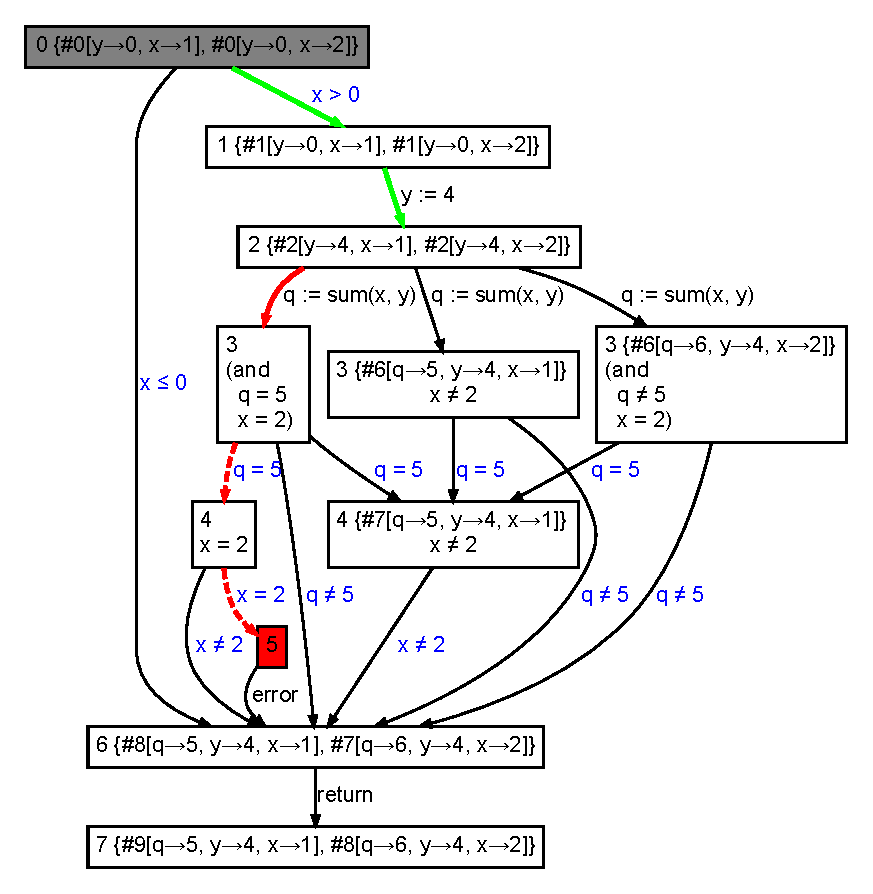
\includegraphics[scale=\scale]{{figs/dashCallcallAddPassExample/27test.graph.5.trace}.eps}
		\label{fig:dashCall:extendFrontier:extractRefinePred:caller}
	}
	\hfil
	\subfloat[$\phi_{ic}$ and $\phi_{ec}$ added to the initial region graph.]
	{
		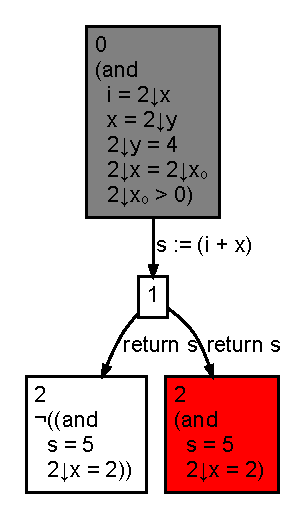
\includegraphics[scale=\scale]{{figs/dashCallcallAddPassExample/28sum.graph.0.init}.eps}
		\label{fig:dashCall:extendFrontier:extractRefinePred:init}
	}
	\hfill
	\subfloat[The only iteration where the initial region is refined.]
	{
		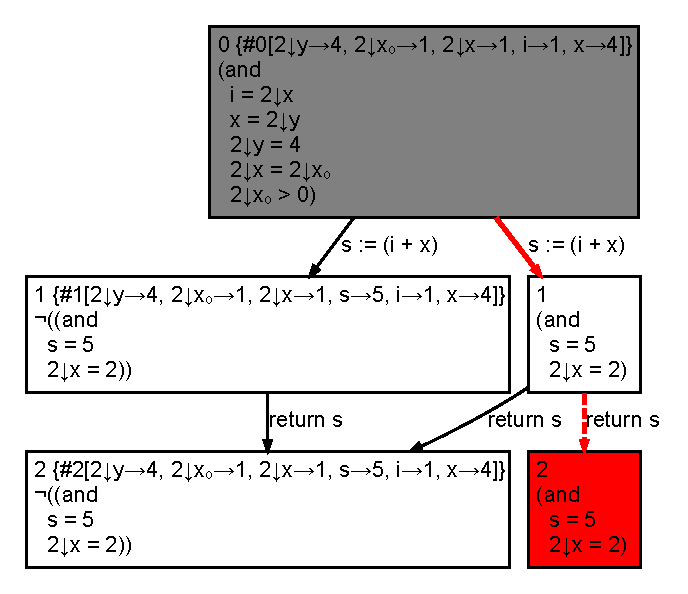
\includegraphics[scale=\scale]{{figs/dashCallcallAddPassExample/36sum.graph.2.trace}.eps}
		\label{fig:dashCall:extendFrontier:extractRefinePred:refineInitial}
	}
	\hfill
	\subfloat[Frontier edge from \protect\subref{fig:dashCall:extendFrontier:extractRefinePred:refineInitial} has been removed.]
	{
		\includegraphics[scale=\scale]{{figs/dashCallcallAddPassExample/37sum.graph.2}.eps}
		\label{fig:dashCall:extendFrontier:extractRefinePred:subDone}
	}
	\caption
	{
		\protect\subref{fig:dashCall:extendFrontier:extractRefinePred:caller} shows an interesting procedure call in regards to computing a refinement predicate. The region graphs \protect\subref{fig:dashCall:extendFrontier:extractRefinePred:init}, \protect\subref{fig:dashCall:extendFrontier:extractRefinePred:refineInitial} and \protect\subref{fig:dashCall:extendFrontier:extractRefinePred:subDone} shows parts of the refinement process completed by \classname{DashLoop} when invoked by \classname{ExtendFrontier}.
	}
	\label{fig:dashCall:extendFrontier:extractRefinePred}
\end{figure}

We will use the procedure call to \code{sum} in \cref{fig:dashCall:extendFrontier:extractRefinePred:caller}, which shows a later iteration of \DASHcall, as an example to illustrate how the refinement predicate $\rho$ is computed. The initial region graph constructed for \code{sum} is shown in \cref{fig:dashCall:extendFrontier:extractRefinePred:init}, and it is impossible to reach the error region in it. This is because the input variable $x$ is required to be 4, because of the input constraint, and the $i$ variable is required to be 2, because of the exit constraint. However, the sum of these two variables stored in $s$ must be 5 if the error region is to be reached, but the sum is always 6. Therefore it is impossible to reach the error region.

The refinement predicate returned from \classname{ExtendFrontier} is based on the predicates that were used to refine the initial region. \cref{fig:dashCall:extendFrontier:extractRefinePred:refineInitial} shows the only trace that results in refinement of the initial region. The trace is infeasible since the path constraint $\phi$ after symbolic execution contains $i_0+x_0=5 \wedge x_0 = 4 \wedge i_0 = 2$, which is unsatisfiable. The refinement predicate used to refine the initial region is computed by using the weakest precondition for the assignment \code{s := i+x} on the frontier edge and the predicate from the region after the frontier:
\begin{align*}
\classname{WP}(\code{s := i+x}, s {=} 5 \wedge 2\rename x {=} 2) 
\is i {+} x {=} 5 \wedge 2\rename x {=} 2
\end{align*}

Refining the initial region with the above predicate results in \cref{fig:dashCall:extendFrontier:extractRefinePred:subDone}. Notice that, as previously described in \cref{sec:dashInt:refinegraph}, when refining the initial region over some edge then that edge is simply removed. An extra requirement is added to \classname{RefineGraph}, such that if it refines the initial region with a predicate, then that predicate is stored in a list on the graph for later retrieval. This is described in \cref{sec:dashCall:refinegraph}.  In the example, the list of predicates that are used to refine the initial region can be seen in the round box with the name ``InitialRefines'' in \cref{fig:dashCall:extendFrontier:extractRefinePred:subDone}.

When \classname{DashLoop} returns with the resulting graph in $z$, all the predicates $\rho_i$ used to refine the initial region is returned by \classname{InitialRefines}. The predicates are combined in a disjunction, and in the example this yields:
\begin{align*}
\bigvee_{\rho_i \in \classname{InitialRefines}(z)}\rho_i 
&\is \bigvee_{\rho_i \in \{(i {+} x {=} 5 \wedge 2\rename x {=} 2)\}}\rho_i \\
&\is \bigvee i {+} x {=} 5 \wedge 2\rename x {=} 2\\
&\is i {+} x {=} 5 \wedge 2\rename x {=} 2
\end{align*}

Again, these predicates are not directly found in the region graph, and have to be maintained separately by \classname{RefineGraph}. In this example the initial region was refined only once, but had it been refined multiple times, then \classname{InitialRefines} would have returned all the predicates used to refine the initial region.

The next step is to substitute all parameters of the called procedure $P'$, with the actual values given in the call. For the call, the variable $x$ is given as the parameter $i$ and the variable $y$ is given for the $x$ parameter. The resulting computation is:
\begin{align*}
&\left(
	\bigvee_{\rho_i \in \classname{InitialRefines}(z)}\rho_i
\right)
\Big[a_0/v_0, \ldots, a_n/v_n\Big]~\mid v_i \in \classname{params}(P') \\
	&\is \Big(i {+} x {=} 5 \wedge 2\rename x {=} 2\Big)\Big[a_0/v_0, \ldots, a_n/v_n\Big]~\mid v_i \in \{i, x\}\\
    &\is \Big(i {+} x {=} 5 \wedge 2\rename x {=} 2\Big)\Big[x/i, y/x\Big]\\
    &\is x {+} y {=} 5 \wedge 2\rename x {=} 2
\end{align*}

The last step is to reverse rename the variables using $\pi^{-1}$:
\begin{align*}
&\rho := \pi^{-1}
	\left(
		\left(
			\bigvee_{\rho_i \in \classname{InitialRefines}(z)}\rho_i
		\right)
		\Big[a_0/v_0, \ldots, a_n/v_n\Big]~\mid v_i \in \classname{params}(P')
	\right)\\
	&\is \pi^{-1}\Big(x {+} y {=} 5 \wedge 2\rename x {=} 2\Big)\\
	&\is x {+} y {=} 5 \wedge x {=} 2
\end{align*}



\begin{figure}
\def \scale {0.52}
	\centering
	\subfloat[The refined region graph resulting from finding that the procedure call in \cref{fig:dashCall:extendFrontier:extractRefinePred:caller} was infeasible.]
	{
		\includegraphics[scale=\scale]{{figs/dashCallcallAddPassExample/40test.graph.6.trace.manualpred}.eps}
		\label{fig:dashCall:extendFrontier:extractRefinePred:done}
	}
	\hfil
	\subfloat[The graph found by the next iteration of \classname{DashLoop} when the trace in \protect\subref{fig:dashCall:extendFrontier:extractRefinePred:done} is found infeasible.]
	{
		\includegraphics[scale=\scale]{{figs/dashCallcallAddPassExample/41test.graph.6.manualpred}.eps}
		\label{fig:dashCall:extendFrontier:extractRefinePred:pass}
	}
	\caption
	{
		Shows the last two refinements of the region graph in \cref{fig:dashCall:extendFrontier:extractRefinePred:caller}.
	}
\end{figure}


This is the refinement predicate $\rho$ returned by \classname{ExtendFrontier}. The idea is that with this predicate, the current trace $\tau_c$ will be eliminated since it was unable to cross the frontier. The refinement predicate has been added in \cref{fig:dashCall:extendFrontier:extractRefinePred:done}. 

The next iteration of \DASHcall will try the trace seen in \cref{fig:dashCall:extendFrontier:extractRefinePred:done}, which is infeasible. The refinement predicate is computed as in \DASHint, since the frontier is not a procedure call. Thus \classname{WP} is used over the assignment \code{y := 4} with the postcondition $x {+} y {=} 5 \wedge x {=} 2$:
\begin{align*}
\classname{WP}(\code{y := 4}, x {+} y {=} 5 \wedge x {=} 2) 
&\is x {+} 4 {=} 5 \wedge x {=} 2\\
&\is \text{\code{false}}
\end{align*}

As can be seen, the refinement predicate is equivalent to \code{false}. When the refinement predicate is used to split region 1, the region graph shown in \cref{fig:dashCall:extendFrontier:extractRefinePred:pass} is created. The error region is unreachable and the analysis stops with \classname{DashLoop} returning \pass. This concludes the \classname{ExtendFrontier} presentation.



\section{\classname{RefineGraph}}
\label{sec:dashCall:refinegraph}
\classname{RefineGraph} is subject to two changes. First the predicates used to split the initial region needs to be recorded. In \cref{alg:dashCall:refinegraph} the procedure \classname{AddInitialRegionSplitPredicate} is used to store those predicates. It has been placed together with the optimization for refining the initial region as described in \cref{sec:dashInt:refinegraph:initialRegion}. 

The second change is to distribute the states in $S_{k-1}$ into $S_{k-1}^*$ and $S_{k-1}^{**}$, since $\rho$ is not as strong as it was in \DASHint. In \DASHint we knew that $\rho$ would always exclude all the known states in $S_{k-1}$. In \DASHcall we only know that it is a suitable predicate, which implies that it will only exclude the states associated with the current trace $\tau_c$. States that are not associated with $\tau_c$, but still resides in $S_{k-1}$ may be able to satisfy $\rho$ and would therefore be placed in $S_{k-1}^{**}$. Remember that there are no requirements that say if $\rho$ is satisfied, then $S_k$ is reached. However, what is required is that if $\rho$ is \textit{not} satisfied, then the error region cannot be reached. The states that are added to $S_{k-1}^{**}$ still does not reach $S_k$, since then the frontier would not have been at the edge $(S_{k-1}, S_k)$.

\begin{thesisalgorithm}
\caption{\classname{RefineGraph}($\rho, \tau_c = \langle RS_0, \ldots, RS_{k-1}, S_k \rangle, G = \langle \Sigma_\simeq, \rightarrow_\simeq \rangle$)}
\label{alg:dashCall:refinegraph}
Returns: $\langle \Sigma_\simeq, \rightarrow_\simeq \rangle$, the refined region graph.

\begin{algorithmic}[1]
	\State \Let $\langle S_{k-1}, \_ \rangle = RS_{k-1}$
	\State \Let $\langle \rho_{k-1}, states \rangle = S_{k-1}$
	\\
	
	\If{$k = 1$}
		\State $\classname{AddInitialRegionSplitPredicate}(\rho)$
		
		\State \Return $\langle \Sigma_\simeq, \rightarrow_\simeq \setminus {(S_{k-1}, S_k)} \rangle$ \Comment{Since k = 1, this is the same as removing $(S_0, S_1)$}
	\EndIf
	
	\\
	
	\State $\Sigma_\simeq^* := \Sigma_\simeq \setminus \{S_{k-1}\}$ \Comment{Remove $S_{k-1}$}
	\State $\rightarrow_\simeq^* := \rightarrow_\simeq \setminus \{(S, S_{k-1}) \mid S \in \classname{Parents}(S_{k-1}) \}$
	\State $\rightarrow_\simeq^* := \rightarrow_\simeq^* \setminus \{(S_{k-1}, S) \mid S \in \classname{Children}(S_{k-1})\}$	
	\\	
	
	\State $\rho_{k-1}^* := \classname{Simplify}(\rho_{k-1} \wedge \neg \rho)$
	\State $\rho_{k-1}^{**} := \classname{Simplify}(\rho_{k-1} \wedge \rho)$

	\For{$s \in states$} \Comment{Distribute states between $S_{k-1}^*$ and $S_{k-1}^{**}$}
		\If{$\classname{Eval}(\rho_{k-1}^*, s) = $ \code{true}}
			\State $states^* := states^* \cup \{s\}$
		\Else
			\State $states^{**} := states^{**} \cup \{s\}$
		\EndIf
	\EndFor
	
	
	\\
	
	\State $S_{k-1}^* := \langle \rho_{k-1}^*, states^* \rangle$
	\State $\Sigma_\simeq^* := \Sigma_\simeq^* \cup \{S_{k-1}^*\}$  \Comment{Insert $S_{k-1}^*$}
	\State $\rightarrow_\simeq^* := \rightarrow_\simeq^* \cup \{(S, S_{k-1}^*) \mid S \in \classname{Parents}(S_{k-1})\}$	
	\State $\rightarrow_\simeq^* := \rightarrow_\simeq^* \cup \{(S_{k-1}^*, S) \mid S \in \classname{Children}(S_{k-1})\}$	
	\\	
	
	
	\State $S_{k-1}^{**} := \langle \rho_{k-1}^{**}, states^{**}  \rangle$
	\State $\Sigma_\simeq^*$ := $\Sigma_\simeq^* \cup \{ S_{k-1}^{**}\}$
	\State $\rightarrow_\simeq^* := \rightarrow_\simeq^* \cup 	\{(S_{k-1}^{**}, S) \mid S \in \classname{Children}(S_{k-1})\}$
	\If{$\classname{IsSAT}(\rho_{k-1}^{**}) = \unsat$} \Comment{Add incoming edges if $\rho_{k-1}^{**}$ is satisfiable}
		\State $\rightarrow_\simeq^* := \rightarrow_\simeq^* \cup \{(S, S_{k-1}^{**}) \mid S \in \classname{Parents}(S_{k-1})\}$
	\EndIf
	
	\\
	
	\State $\rightarrow_\simeq^* := \rightarrow_\simeq^* \setminus \{(S_{k-1}^*, S_k)\}$ \Comment{Remove frontier edge from $S_{k-1}^*$}
	\State \Return $\langle \Sigma_\simeq^*, \rightarrow_\simeq^* \rangle$
\end{algorithmic}
\end{thesisalgorithm}

\section{Finding error statements in sub procedures}
\label{sec:dashCall:errorInSubprocedures}
As mentioned in the start of this chapter, \DASHcall only finds the \code{error} statements in the top level procedure of a multi-procedure program. The \DASH article specifically mentions:
\begin{thesisquote}{Page 11 in \DASH~\cite{dash2010}}
	We will assume without loss of generality that the property $\phi$ that we wish to check is only associated with the main procedure $P_0$ in the program $\mathpzc{P}$.
\end{thesisquote}

The \DASH algorithm, as described in the \DASH article, supports pointers into the heap and as such global state. Using global state, the limitation that \code{error} statements can only occur in the main procedure can be avoided with a clever instrumentation. We believe that the authors of \DASH thought of this instrumentation when they wrote \textit{without loss of generality}. Essentially all calls to \code{error} in sub procedures are replaced with an assignment \code{ERROR = 1} to a global variable \code{ERROR}. The main procedure is then instrumented to check if \code{ERROR} has been set to 1. If this is the case, then the main procedure executes the \code{error} statement to signal the failure. 

The instrumentation process is illustrated in \cref{fig:dashCall:errorInSubProcedures}. \cref{fig:dashCall:errorInSubProcedures:before} shows two procedures where \code{main} is the main procedure and \code{sub} is a sub procedure called by \code{main}. Notice that \code{sub} uses the \code{error} statement, which \DASH does not support. \cref{fig:dashCall:errorInSubProcedures:after} shows the same code, but instrumented to use a global variable \code{ERROR} to signal to the main procedure when \code{sub} has reached an error. As such it does not matter that only \code{error} statements in the main procedure are searched for by \DASH, at least not if global state is supported. However, since \DASHcall does not support global state, we cannot use this instrumentation process for programs analyzed by \DASHcall.

\begin{figure}
\newsavebox{\dashErrorInSubProcedureBeforeInstrumentation}
\begin{lrbox}{\dashErrorInSubProcedureBeforeInstrumentation}
\begin{lstlisting}


int main(int x, int y)
{
	return sub(x, y);
	
	
	
}

int sub(int a, int b)
{
	if(a * 4 > b)
		error;
	return a + b;
}
\end{lstlisting}
\end{lrbox}
\newsavebox{\dashErrorInSubProcedureAfterInstrumentation}
\begin{lrbox}{\dashErrorInSubProcedureAfterInstrumentation}
\begin{lstlisting}
GLOBAL int ERROR = 0;

int main(int x, int y)
{
	int r = sub(x, y);
	if(ERROR == 1)
		error;
	return r;
}

int sub(int a, int b)
{
	if(a * 4 > b)
		ERROR = 1;
	return a + b;
}
\end{lstlisting}
\end{lrbox}

\centering
\subfloat[Before instrumentation]
{
	\usebox{\dashErrorInSubProcedureBeforeInstrumentation}
	\label{fig:dashCall:errorInSubProcedures:before}
}
\hfil
\subfloat[After instrumentation]
{
	\usebox{\dashErrorInSubProcedureAfterInstrumentation}
	\label{fig:dashCall:errorInSubProcedures:after}
}
\caption
{
	\protect\subref{fig:dashCall:errorInSubProcedures:before} shows two procedures where the \code{sub} procedure uses an \code{error} statement. \DASH only supports \code{error} statements in the main procedure. Using global state \code{error} statements in sub procedures can be avoided as is seen in \protect\subref{fig:dashCall:errorInSubProcedures:after}.
}
\label{fig:dashCall:errorInSubProcedures}
\end{figure}

\section{Challenges and modifications}
\label{sec:dashCall:challenges}
This section summarizes the challenges and modifications we have made to the \DASH algorithm, when handling programs that support integer variables and procedure calls.

\subsection{Infinite refinement when the frontier is a procedure call}
\label{sec:dashCall:infiniteRefineAtProc}
We have had a number of problems when incorporating the loop optimization from \DASHint while adding procedure calls. We found that some of our test cases went into an infinite refine loop, when refining over a procedure call. The problems we describe here arose before we had introduced the optimization that removes the frontier edge when refining the initial region, and it was also before we disallowed the use of the loop optimization on the initial region. 

We present an example where infinite refinement occurs over a procedure call edge. The two procedures in the example are shown in \cref{fig:dashCall:infiniteRefineAtProcProblem:test} and \cref{fig:dashCall:infiniteRefineAtProcProblem:abs}. The \code{test} procedure is the main procedure. The problem is that the same edge is continuously refined with the same input and exit constraints. This results in multiple new initial regions that have the region predicate \code{false} and are therefore unsatisfiable.

\begin{figure}
\def \height {4.5cm}

\newsavebox{\dashCallInfiniteRefinementAtProcedureCallEdgeTest}
\begin{lrbox}{\dashCallInfiniteRefinementAtProcedureCallEdgeTest}
\begin{lstlisting}[mathescape]
void test(int k)
{
    int a = abs(k);
    if(a < 0)
        if(a $\neq$ -2147483648)
            error;
}
\end{lstlisting}
\end{lrbox}
\newsavebox{\dashCallInfiniteRefinementAtProcedureCallEdgeAbs}
\begin{lrbox}{\dashCallInfiniteRefinementAtProcedureCallEdgeAbs}
\begin{lstlisting}[mathescape,showlines]
int abs(int z)
{
    if (z < 0)
        return -z;
    return z;
}

\end{lstlisting}
\end{lrbox}

\subfloat[test procedure]
{
	\usebox{\dashCallInfiniteRefinementAtProcedureCallEdgeTest}
	\label{fig:dashCall:infiniteRefineAtProcProblem:test}
}
\quad\quad
\subfloat[abs procedure]
{
	\usebox{\dashCallInfiniteRefinementAtProcedureCallEdgeAbs}
	\label{fig:dashCall:infiniteRefineAtProcProblem:abs}
}
\hfil
\subfloat[About to analyze sub procedure]
{
	\includegraphics[height=\height]{{figs/infiniteRefineAtProc/46test.graph.5.trace}.eps}
	\label{fig:dashCall:infiniteRefineAtProcProblem:beforeFirstRefine}
}
\hfil
\subfloat[About to analyze sub procedure]
{
	\includegraphics[height=\height]{{figs/infiniteRefineAtProc/80test.graph.6.trace}.eps}
	\label{fig:dashCall:infiniteRefineAtProcProblem:afterFirstSplit}
}
\hfil
\subfloat[First \code{false} region arises]
{
	\includegraphics[height=\height]{{figs/infiniteRefineAtProc/111test.graph.7.trace}.eps}
	\label{fig:dashCall:infiniteRefineAtProcProblem:oneFalse}
}
\hfil
\subfloat[More \code{false} regions arises]
{
	\includegraphics[height=3.5cm]{{figs/infiniteRefineAtProc/204test.graph.10.trace}.eps}
	\label{fig:dashCall:infiniteRefineAtProcProblem:manyFalse}
}
\caption
{
	Shows the problem of infinite loop refinement. Code is shown in \protect\subref{fig:dashCall:infiniteRefineAtProcProblem:test} and \protect\subref{fig:dashCall:infiniteRefineAtProcProblem:abs}.
	In \protect\subref{fig:dashCall:infiniteRefineAtProcProblem:beforeFirstRefine} we are about to refine a procedure call edge. \protect\subref{fig:dashCall:infiniteRefineAtProcProblem:afterFirstSplit} shows the graph after refinement and together with \protect\subref{fig:dashCall:infiniteRefineAtProcProblem:oneFalse} shows the infinite loop forming, due to the same input and exit constraints. \protect\subref{fig:dashCall:infiniteRefineAtProcProblem:manyFalse} shows the graph after a couple of refinements and the infinite loop is in progress.
}

\label{fig:dashCall:infiniteRefineAtProcProblem}
\end{figure}

The trace in \cref{fig:dashCall:infiniteRefineAtProcProblem:beforeFirstRefine} has the procedure call to \code{abs} as the frontier. \classname{DashLoop} is invoked and because no input values can satisfy the exit constraint, we expect to find the refinement predicate to be, or equivalent to, \code{false}. No values that \code{abs} can take will satisfy the exit constraint, since as seen earlier, the only way \code{abs} can return a negative value, is by passing it $-2{,}147{,}483{,}648$ as input. However this value is specifically disallowed in the exit constraint and therefore the exit constraint $a<0 \wedge a \neq -2{,}147{,}483{,}648$ is impossible to satisfy. The suitable refinement predicate returned should therefore be \code{false}, but as we can see in \cref{fig:dashCall:infiniteRefineAtProcProblem:afterFirstSplit} the found refinement predicate returned is actually $(k \neq -2{,}147{,}483{,}648 \wedge k < 0) \vee (k \neq -2{,}147{,}483{,}648 \wedge k > 0)$, which we name $\rho^*$.

In the next iteration of \DASH the procedure call is still the frontier, but now additional input constraints are given when analyzing \code{abs}. However, \classname{DashLoop} finds the same refinement predicate $\rho^*$, with the result of splitting the initial region in two. One with the predicate $\rho^* \wedge \neg \rho^*$ and one with the predicate $\rho^* \wedge \rho^*$. The first predicate is equivalent to \code{false}, with the second being identical to the original predicate, and thus no progress is achieved. This is shown in \cref{fig:dashCall:infiniteRefineAtProcProblem:oneFalse}. The refinement predicate returned is not suitable, which seems to be the root cause of the infinite refinement problem. The infinite loop has begun, where additional initial regions with the predicate \code{false} are added, as can be seen in \cref{fig:dashCall:infiniteRefineAtProcProblem:manyFalse}.

We tried a number of techniques, which either did not work or it was unknown why they worked, to solve the problem:
\begin{itemize}
	\item Completely disabling the loop optimization solved the problem, which also served to confirm our belief that the problem arose because we found and used a refinement predicate that was not suitable. However, without the loop optimization, some of the test cases for \DASHint failed.

	\item At this point in time, our \classname{RefinePred} implementation was allowed to use the loop optimization, even if there were no states in a region that was moved. We tried to add the requirement that at least one state should be moved, as argued for earlier in \cref{sec:dashInt:challenges:howToImplementLoopOptimization:initialRegion}. This fixed some of the tests that failed, but others, like the example presented in this section, still failed.

	\item Another solution we came up with, was the idea that an edge going out of the initial region could simply be removed if the SAT solver found it infeasible. This solved the problem for all our test cases. However we were unable to explain why this solution should solve the problem, and we were hesitant to use it.
\end{itemize}

We found the final solution while arguing that the predicate computed by \classname{ExtendFrontier} in \cref{sec:dashCall:extendFrontier:ExtractResult}, when \classname{DashLoop} found the error regions to be unreachable in a sub procedure, was actually a suitable refinement predicate. The argument only worked if we assumed that all the refinement predicates that were used to refine the initial region in the sub procedure were suitable predicates. If the predicates were suitable, then we could show that the computed predicate would be suitable for the original procedure. This resulted in changing \classname{RefinePred} such that the loop optimization could never be used when it was the initial region that was being refined. We introduced it in \DASHint, in \cref{sec:dashInt:refinePred}, since it also fixes the problem in \cref{sec:dashInt:challenges:infiniteRefinementWithLoopOptimziation}. In this way, the infinite refinement problem for the example presented in this section was solved. The refinement predicate returned was forced to be suitable, and therefore progress was achieved.

Our implementation still uses the idea of removing outgoing edges from the initial region when they are refined. However, we have tested that if we allow multiple initial regions, the solution where the loop optimization is disallowed on initial regions still works for all our test cases. Therefore, removing edges when refining the initial region is only an optimization that simplifies the presentation in this thesis, such that the graphs presented are smaller.

\subsection{Lack of path constraint in the input constraint}
\label{sec:dashCall:challenges:lackOfPathConstraint}
We have had major problems adding interprocedural analysis to \DASHint. This section describes the key problems with invoking \classname{DashLoop} from inside \classname{ExtendFrontier}. The \DASH article uses approximately one page on describing modifications of \classname{ExtendFrontier} and some additional helper procedures. However, we have had to modify code in many places to get \DASHint to handle interprocedural analysis. One of the biggest problems we have had was how to construct the input and exit constraints given to \classname{DashLoop}, when invoking it from inside \classname{ExtendFrontier}.

The original pseudocode for \classname{ExtendFrontier} that can handle interprocedural analysis is shown in \cref{alg:dashCall:challenges:extendFrontierOriginal}. \cref{sec:dashCall:challenges:lackOfGetWholeAbstractTrace} describes that they take a trace that traverses only the analyzed procedure and constructs a full trace that traverses sub procedures using a call to \classname{GetWholeAbstractTrace}.

\begin{thesisalgorithm}
\caption{\classname{ExtendFrontier}$_{original}(\tau_o, F, P)$ for interprocedural analysis}
\label{alg:dashCall:challenges:extendFrontierOriginal}
Returns:\\
$\langle t,$ \code{true}$\rangle$, if the frontier can be extended; or\\
$\langle \unsat, \rho \rangle$, if the frontier cannot be extended\\

\begin{algorithmic}[1]
	\State $\tau_w = \langle S_0, S_1, \ldots, S_n \rangle := \classname{GetWholeAbstractTrace}(\tau_o, F)$
	\State $(k-1, k) := \classname{Frontier}(\tau_w)$
	\State $\langle \phi_1, \mathpzc{S}, \phi_2 \rangle := \classname{ExecuteSymbolic}(\tau_w, P)$
	\If{$\classname{Edge}(S_{k-1}, S_k) \in \classname{CallReturn}(E)$}

		\State \Let $\langle \Sigma, \sigma^I, \rightarrow \rangle=\classname{GetProc}(\classname{Edge}(S_{k-1},S_k))$
		\State $\phi := \classname{InputContraints}(\mathpzc{S})$
		\State $\phi' := S_k[e/x]$
		\State $\langle r, m \rangle := \classname{DASH}( \langle \Sigma, \sigma^I \wedge \phi, \rightarrow \rangle, \neg \phi')$

		\If{$r = \fail$}
			\State $t := m$
			\State $\rho :=$ \code{true}
		\Else
			\State $\rho := \classname{ComputeRefinePred}(m)$
			\State $t := \unsat$
		\EndIf

	\Else	

		\State $t := \classname{IsSAT}(\phi_1, \mathpzc{S}, \phi_2, P)$
		\If{$t = \unsat$}
			\State $\rho := \classname{RefinePred}(\mathpzc{S}, \tau_w)$
		\Else
			\State $\rho :=$ \code{true}
		\EndIf

	\EndIf
	\State \Return $\langle t, \rho \rangle$
\end{algorithmic}
\end{thesisalgorithm}

They construct the input constraint in line 6 with a call to \classname{InputConstraints} giving the symbolic map $\mathpzc{S}$ as the only argument. They write the following about the input constraint in the article:

\begin{thesisquote}{Page 11 in \DASH~\cite{dash2010}}
	The predicate $\phi$ corresponds to the constraints on $Q$'s input variables which are computed directly from the symbolic memory $\mathpzc{S}$ (by the auxiliary function \classname{InputConstraints} at line 7), [\ldots].
\end{thesisquote}

A small typo in their quote exists, since \classname{InputConstraints} is actually called in line 6. What is more severe is that they write that the input constraint for the called procedure $Q$ can be computed directly from what we call the symbolic map $\mathpzc{S}$. As we know by now, the symbolic map contains mappings of the form $v \mapsto e$ where $e$ can be a constant or a symbolic expression. Thus the constraint they generate must be in the form $p_1 = \classname{SymbolicEval}(a_1, \mathpzc{S}) \wedge \ldots \wedge p_n = \classname{SymbolicEval}(a_n, \mathpzc{S})$ where $p_i$ are the parameter names and $a_i$ is the argument given for $p_i$. The path constraint is missing from this input constraint. There is no way to include the path constraint from the trace $\tau_c$ by using only the symbolic map $\mathpzc{S}$, since $\mathpzc{S}$ only contains a snapshot of the program state at region $S_{k-1}$. The path constraint is located in $\phi_1$ and is \textit{not} given to \classname{InputConstraints}.

Our first implementation followed their pseudocode and explanations. However, we found cases where this led to problems. We had two distinct problems:

1) When \classname{DashLoop} returns with a test input for the sub procedure, then that test input might not include all the variables needed to call the callee procedure. This happens when a variable is used in an \code{if} expression but not given as an argument to the sub procedure. An example is given in \cref{fig:dashCall:challenges:callNotAllVariablesGiven}. The $y$ variable cannot be zero if \code{abs} is to be called. However, when analyzing \code{abs} the path constraint is not added to the input constraint and the result of the analysis will not even include a value for $y$. If the default value of zero is used, the execution will not follow $\tau_c$ nor cross the frontier.

One can solve this problem by using an \classname{IsSAT} call. The problem given to \classname{IsSAT} is simply $\phi_1$ and where all the arguments are assigned the solutions in $t$. Thus if $x$ has to be 4, then the extra constraint $x = 4$ must be added to $\phi_1$. However, this solution does not solve the next problem we discovered.

\begin{figure}
\newsavebox{\dashCallProblemsCallNotAllVariablesGiven}
\begin{lrbox}{\dashCallProblemsCallNotAllVariablesGiven}
\begin{lstlisting}[mathescape]
void testabs(int x, int y)
{
	if(y $\neq$ 0)
	{
		x = abs(x);
		if(x < 0)
			error;
	}
}
\end{lstlisting}
\end{lrbox}

\newsavebox{\dashCallProblemsCallWithPrecondition}
\begin{lrbox}{\dashCallProblemsCallWithPrecondition}
\begin{lstlisting}[mathescape]
void testabs2(int x)
{
	if(x $\neq$ -2147483648)
	{
		x = abs(x);
		if(x < 0)
			error;
	}
}
\end{lstlisting}
\end{lrbox}

\newsavebox{\dashCallProblemsCallAbs}
\begin{lrbox}{\dashCallProblemsCallAbs}
\begin{lstlisting}[mathescape,showlines]
int abs(int a)
{
	if (a < 0)
		return -a;
	return a;
}



\end{lstlisting}
\end{lrbox}
\centering

\subfloat[]
{
	\usebox{\dashCallProblemsCallNotAllVariablesGiven}
	\label{fig:dashCall:challenges:callNotAllVariablesGiven}
}
\hfil
\subfloat[]
{
	\usebox{\dashCallProblemsCallWithPrecondition}
	\label{fig:dashCall:challenges:callWithPrecondition}
}
\hfil
\subfloat[]
{
	\usebox{\dashCallProblemsCallAbs}
	\label{fig:dashCall:challenges:callAbs}
}
\caption
{
	\protect\subref{fig:dashCall:challenges:callNotAllVariablesGiven} shows the \code{testabs} procedure which calls the \code{abs} procedure in \protect\subref{fig:dashCall:challenges:callAbs} whenever $y \neq 0$.
	\protect\subref{fig:dashCall:challenges:callWithPrecondition} shows the \code{testabs2} procedure which has a precondition on $x$ that it must not be the smallest negative value. Analyzing these procedures with the constraints calculated by \classname{InputConstraints} produces meaningless solutions.
}
\end{figure}

2) If some variables are constrained by the path constraint prior to a procedure call, such as in an \code{if} condition, then the procedure analysis might come up with an input parameter that conflicts with the path constraint, since it is not given when analyzing the called procedure. An example is given in \cref{fig:dashCall:challenges:callWithPrecondition}. Here the \code{testabs2} procedure calls the \code{abs} procedure with the argument $x$. At the point of the call $x$ can be any value except for the smallest possible value $-2{,}147{,}483{,}648$. This value is the only value that allows \code{abs} to return a negative value. Therefore it is not possible to reach the \code{error} statement in the \code{testabs2} procedure. However, when analyzing the \code{abs} procedure, the requirement given is that it must return a negative value, such that the \code{error} statement can be reached. The result returned is that \code{abs} should be called with $-2{,}147{,}483{,}648$, as was discovered in the \DASHint complete example from \cref{sec:dashInt:completeExample}. However, the \code{testabs2} procedure is unable to call \code{abs} with that specific value, since the path constraint prohibits it.

These two examples shows that constructing the input constraint solely from the symbolic map $\mathpzc{S}$ cannot be correct. The solution to the above problems was to add the path constraint together with the arguments from the symbolic map. However, there are cases where the exit constraint contains variables that are not given in either the path constraint or the arguments to the called procedure. 

The two procedures in \cref{fig:dashCall:challenges:callMustDumpSymbolicMap} shows that it is not enough to only add the symbolically evaluated arguments from the symbolic map to the input constraint $\phi_{ic}$ when analyzing the called procedure. The \code{foo} procedure can reach the \code{error} statement if $x$ is equal $y$. The procedure starts by assigning 4 to $y$ and thereafter \code{zero} is called, which returns zero. Thus $x$ is always 0 and $y$ always 4 which makes the \code{error} statement unreachable.

\begin{figure}
\newsavebox{\dashCallProblemsCallMustDumpSymbolicMapFoo}
\begin{lrbox}{\dashCallProblemsCallMustDumpSymbolicMapFoo}
\begin{lstlisting}[mathescape]
void foo()
{
	int y = 4;
	int x = zero();
	if(x == y)
		error;
}
\end{lstlisting}
\end{lrbox}
\newsavebox{\dashCallProblemsCallMustDumpSymbolicMapZero}
\begin{lrbox}{\dashCallProblemsCallMustDumpSymbolicMapZero}
\begin{lstlisting}[mathescape,showlines]
int zero()
{
	return 0;
}



\end{lstlisting}
\end{lrbox}
\centering

\subfloat[]
{
	\usebox{\dashCallProblemsCallMustDumpSymbolicMapFoo}
	\label{fig:dashCall:challenges:callMustDumpSymbolicMap:foo}
}
\hfil
\subfloat[]
{
	\usebox{\dashCallProblemsCallMustDumpSymbolicMapZero}
	\label{fig:dashCall:challenges:callMustDumpSymbolicMap:zero}
}
\caption
{
	Example where including both the path constraint and the arguments from the symbolic map is not enough for correct analysis. The whole symbolic map must be included in the input constraint to \code{zero}.
}
\label{fig:dashCall:challenges:callMustDumpSymbolicMap}
\end{figure}

Analyzing \code{foo} would proceed by executing a concrete test, which does not reach the \code{error} statement. The trace found in the next iteration has the frontier edge going into the error region. The trace is found infeasible. The next iteration has a trace where the frontier edge is over the \code{zero} procedure call. In this case the exit constraint is $x = y$, but $y$ is not part of either the path constraint or the arguments given to the \code{zero} procedure. If a default value of zero is assigned to $y$ since it is not constrained, then the analysis reports that the trace is feasible, which it is clearly not. The problem is that the analysis of the sub procedure cannot see that $y$ must be 4.

Problems can also arise when a test is executed with \classname{RunTest} and a variable in the exit constraint is not mentioned in either the path constraint or in arguments. \classname{IsSAT} then does not find a value for the variable, which causes \classname{RunTest} to be unable to evaluate a region predicate that contains the variable.

The conclusion is that \DASH has to dump the whole symbolic map into the input constraint together with the path constraint. This is also how we presented the computation of the input constraint in \cref{sec:dashCall:extendFrontier:inputconstraint}.

We have later learned, by personal correspondence, that the \DASH implementation actually asserts the path constraint to \Zthree prior to analyzing a sub procedure. In this way, they achieve the same effect as if the input constraint contained the path constraint. However, we do not know how they add constraints from the symbolic map.

\subsection{Problem: Handling of recursive procedures}
\label{sec:dashCall:challenges:recursiveProcedures}
As was mentioned in the introduction to this chapter, \DASHcall is unable to handle certain types of recursive invocations. The \DASH article contains the following paragraph describing how it handles recursive procedures:

\begin{thesisquote}{Page 12 in \DASH~\cite{dash2010}}
	If a procedure needs to be recursively invoked in order to reach an error condition, \DASH itself will be recursively invoked, substituting appropriate values for concrete parameters, so that symbolic execution will eventually ``bottom out'', in the base case of the recursion. On the other hand, if the recursive execution of a procedure is not directly related to the error, the algorithm will generate test cases that pass right though the recursive invocations, at which point the call will be on the near side of the frontier.
\end{thesisquote}

It thus seems like the \DASH algorithm has no problems with recursive procedures and does not need any kind of special handling for it. For the example given in \cref{fig:dashCall:challenges:recursive:bound} \DASH quickly terminates finding the input $x \mapsto 2$, which is the value that \code{fib(3)} returns. Thus, the error region is quickly reached.

However, we have found examples where \classname{DashLoop} is recursively invoked infinitely, i.e. no automatic ``bottoming out'' in any base cases.

The \code{free} procedure given in \cref{fig:dashCall:challenges:recursive:free} results in infinite analysis. The \code{error} statement cannot be reached since \code{fib(0)} is zero ($x$ needs to be zero to satisfy the \code{if} condition). However, since $x$ is not bound to any specific value, \DASH keeps recursively invoking \classname{DashLoop}, never bottoming out. We have not found any solution to this problem.

\begin{figure}
\newsavebox{\dashCallProblemsRecursiveTestBound}
\begin{lrbox}{\dashCallProblemsRecursiveTestBound}
\begin{lstlisting}[mathescape,showlines]
void bound(int x)
{
	int f = fib(3);
	if(f == x)
		error;

}
\end{lstlisting}
\end{lrbox}
\newsavebox{\dashCallProblemsRecursiveTestFree}
\begin{lrbox}{\dashCallProblemsRecursiveTestFree}
\begin{lstlisting}[mathescape]
void free(int x)
{
	int f = fib(x);
	if(f == 1)
		if(x == 0)
			error;
}
\end{lstlisting}
\end{lrbox}
\newsavebox{\dashCallProblemsRecursiveFib}
\begin{lrbox}{\dashCallProblemsRecursiveFib}
\begin{lstlisting}[mathescape]
int fib(int i)
{
	if (i == 0) return 0;
	if (i $\leq$ 2) return 1;
	return fib(i - 1) +
	       fib(i - 2);
}
\end{lstlisting}
\end{lrbox}
\centering

\subfloat[]
{
	\usebox{\dashCallProblemsRecursiveTestBound}
	\label{fig:dashCall:challenges:recursive:bound}
}
\hfil
\subfloat[]
{
	\usebox{\dashCallProblemsRecursiveTestFree}
	\label{fig:dashCall:challenges:recursive:free}
}
\hfil
\subfloat[]
{
	\usebox{\dashCallProblemsRecursiveFib}
	\label{fig:dashCall:challenges:recursive:fib}
}
\caption
{
	The \code{bound} procedure in \protect\subref{fig:dashCall:challenges:recursive:bound} calls the recursive procedure \code{fib} given in \protect\subref{fig:dashCall:challenges:recursive:fib} with a bound constant. \DASH quickly finds a test for \code{bound} that reaches the error. The \code{free} procedure in \protect\subref{fig:dashCall:challenges:recursive:free} calls \code{fib} with a free unconstrained variable, which makes \DASH enter an infinite recursive analysis.
}
\label{fig:dashCall:challenges:recursive}
\end{figure}

\subsection{\classname{GetWholeAbstractTrace}: confusing}
\label{sec:dashCall:challenges:lackOfGetWholeAbstractTrace}
The \classname{ExtendFrontier} procedure presented in the \DASH article, reproduced as \cref{alg:dashCall:challenges:extendFrontierOriginal}, shows that the procedure \classname{GetWholeAbstractTrace} is used. The authors describe the functionality as:

\begin{thesisquote}{Page 11 in \DASH~\cite{dash2010}}
	\classname{ExtendFrontier} first calls the auxiliary function \classname{GetWholeAbstractTrace} (line 1). \classname{GetWholeAbstractTrace} takes an ordered abstract error trace $\tau = \langle S_0, S_1, \ldots, S_n \rangle$ and a forest $F$ as input, and returns an ``expanded'' whole abstract error trace $\tau_w$. Essentially, $\tau_w$ is the abstract trace $\tau$ with all call-return edges up to its frontier replaced with the abstract trace traversed in the called function (and this works in a recursive manner), so that it is really a trace of every abstract program point through which the test passed. If $\classname{Edge}(S_i, S_{i+1})$ is a call-return edge that occurs before the frontier, \classname{GetWholeAbstractTrace} runs a test $t$ (obtained from the concrete witness in $S_i$) on the called procedure $\classname{GetProc}(e)$ and replaces $\classname{Edge}(S_i, S_{i+1})$ with the sequence of regions corresponding to the test $t$.
\end{thesisquote}

Thus they create a trace that passes through every program point in both the main procedure and through the called sub procedures. There are multiple problems to this approach:

\begin{itemize}
	\item The trace $\tau_w$ is a list of regions where all call-return edges $(S_i, S_{i+1})$ have been replaced with $S_{t1}, \ldots, S_{tn}$ originating from the test $t$. It is not given which operation exists on the edges $(S_i, S_{t1})$ and $(S_{tn}, S_{i+1})$.
	
	\item A call return edge $(S_i, S_{i+1})$ cannot be replaced without explicit handling of arguments and parameters. If $x$ is passed to a procedure as the parameter $y$ then there must be an assignment of some form to convey that $x$ and $y$ are connected. The same problem exists for \code{return} statements.
	
	\item What happens when there are two procedures that both takes $x$ as a parameter. They do not touch upon renaming of variables while describing \classname{GetWholeAbstractTrace}.
	
	\item As we have understood the \DASH algorithm, they maintain a forest $F$ for each procedure in the program. They write ``As in the single procedure case, we maintain a forest $F$ and an abstraction $P_\simeq$ for every procedure $P$ in the program.''\footnote{Page 11 in \DASH~\cite{dash2010}} They should therefore be able to lookup the correct path in one of the forests and thereby not need to execute a test $t$ to figure out the path taken by $\tau$ in the sub procedure.
\end{itemize}

They also mention that only \classname{ExtendFrontier} needs to be altered for interprocedural analysis to function. Given the above listed problems we cannot see how \classname{ExecuteSymbolic} should be able to execute $\tau_w$ without modifications. Also, as should have been evident from our presentation, we have concrete states attached to the region graph of sub procedures such that following the trace $\tau$ was a simple task for us.

Our pseudocode for \classname{ExecuteSymbolic}, shown in \cref{alg:dashCall:executeSymbolic}, handles: 1) following the trace, 2) arguments/parameters, 3) return values and finally it uses a symbolic map for each sub procedure such that renaming is not needed. Our first implementation actually did perform renaming, but when we wrote down the pseudocode for it, we found that renaming could be avoided and recoded our implementation.

All in all, it seems that \classname{GetWholeAbstractTrace} is a procedure that is used to compact the presentation of the \DASH interprocedural algorithm. The real \DASH implementation probably does something similar to what we do.

\subsection{Consequences of having states on regions}
The \DASH authors maintains a forest $F$ for every procedure, as is evident in the quote below:

\begin{thesisquote}{Page 11 in \DASH~\cite{dash2010}}
	As in the single procedure case, we maintain a forest $F$ and an abstraction $P_\simeq$ for every procedure $P$ in the program.
\end{thesisquote}

A major difference between our implementation and their pseudocode is that our version keeps the abstraction $P_\simeq$ and the forest $F$ together in the region graph data structure. They invoke \classname{DashLoop} with an empty forest and a fresh abstraction. Thus, when we need to invoke \classname{DashLoop} all the concrete states must be removed from the region graph, such that the sub procedure gets a fresh start.

\subsection{\classname{ComputeRefinePred}: confusions about $\rho_i$ and $\neg$}
In the \DASH article, the procedure \classname{ComputeRefinePred} is responsible for computing the refinement predicate for $P$ in \classname{ExtendFrontier} when \classname{DashLoop} has proved that no error regions are reachable in the sub procedure $P'$. Our computation for \classname{ComputeRefinePred} differs from the one presented in the \DASH article. We have used:
\begin{align*}
\rho := \bigvee_{\rho_i \in \classname{InitialRefines}(z)}\rho_i
\end{align*}
given that we ignore reverse renaming and argument/parameter substitution. We have argued in \cref{sec:dashCall:extendFrontier:ExtractResult} for why this is a suitable predicate that can be used to eliminate $\tau_c$ in $P$. In the article the authors use the following definition:
\begin{thesisquote}{Page 12 in \DASH~\cite{dash2010}}
Specifically, $\classname{ComputeRefinePred}(m)$ is defined as follows.
\begin{align*}
\classname{ComputeRefinePred}(m) := \neg \bigvee \rho_i
\end{align*}
where each $\rho_i$ is a predicate in the proof $m$ used to split the initial region $\sigma^I \wedge \phi$. It can be shown that \classname{ComputeRefinePred} returns a suitable predicate.
\end{thesisquote}

Immediately it can be seen that we have removed a negation ($\neg$) from the definition. Additionally we have discovered, by personal correspondence, that the $\rho_i$ they use in their definition are not actually the predicates returned by \classname{RefinePred}, but are the predicates that would be attached to the initial region. Those predicates are the negated versions of those returned by \classname{RefinePred}. Thus, their $\rho_i$, which we call $\rho_{i_{their}}$, is actually the negated version of our $\rho_i$'s, which we can call $\rho_{i_{our}}$. We can express the difference by the equation $\rho_{i_{their}} = \neg \rho_{i_{our}}$. We assumed that $\rho_i$ referred to the suitable predicate returned by \classname{RefinePred}, since $\rho$ has been used as such in the previous sections of the article. If we insert their definition of $\rho_i$ in \classname{ComputeRefinePred} we get:
\begin{align*}
\classname{ComputeRefinePred}(m) &:= \neg \bigvee \rho_{i_{their}}\\
	&:= \neg \bigvee \neg \rho_{i_{our}}\\
	&:= \bigwedge \rho_{i_{our}}
\end{align*}
This still does not match our definition. They use a conjunction where we use a disjunction. What is worse, is that this predicate is not a suitable predicate for $\tau_c$ in the caller procedure $P$. Remember, that for a predicate to be suitable with respect to $\tau_c$, the negated version must disallow any state to reach the region after the frontier. This is a requirement since then we are allowed to remove an edge when splitting $S_{k-1}$ into two. However, their negated version:
\begin{align*}
\neg\bigwedge \rho_{i_{our}} \is \bigvee \neg\rho_{i_{our}}
\end{align*}
basically means that if a single $\rho_{i_{our}}$ is not satisfied, it is not possible to reach $S_k$. However, it might be possible to reach one of the error regions in $P'$ as long as one of the $\rho_{i_{our}}$'s is satisfied. Therefore, their predicate is not a suitable refinement predicate. This makes a difference when the initial region in $P'$ has been refined multiple times, such that there is more than one $\rho_i$. It also makes a difference when the initial region in $P'$ has not been refined at all. Then their predicate becomes \code{true}, since it is neutral element for conjunction, but with \code{true}, progress is not achieved.

We do not believe that they use the above formula. There must be some mismatch in the communication between us and the authors of \DASH, either in the article or by personal correspondence.

%%%%%%%%%%%%%%%%%%%%%%%%%%%%%%%%%%%%%%%%%%%%%%%%%%%%%%%%%%%%%%%%%%%%%%%

\chapter{Implementation details when implementing DASH$_{call}$ in \Java for analyzing a subset of \Java}
\label{ch:dashImplementation}
This chapter describes the implementation details of \DASHcall. We have named the implementation \DASH for \Java, or in short form \DASHforj. \DASHforj takes as input a small \Java program and analyses it as \DASHcall would. Our implementation code is structured to resemble the pseudocode presented for \DASHcall. There are some practical obstacles that need to be solved before all the requirements for the \DASHcall algorithm are met:

\begin{itemize}
	\item \Java code needs to be loaded. There is a difference between what \DASH supports and what \Java supports. For example, \DASH does not support expressions with side effects, but \Java does with the syntax \code{i++}.
	
	\item A SAT solver is needed for the \classname{IsSAT} procedure.
	
	\item A region graph must be constructed for \DASH analysis.
	
	\item \classname{RunTest} must be able to execute a test and collect states for the region graph.
\end{itemize}

The supported \Java features are described in \cref{sec:dashImpl:supportedFeatures}. Desugaring of \Java code is described in \cref{sec:dashImpl:jimple} whereas construction of region graphs is presented in \cref{sec:dashImpl:regionGraph}. We use instrumentation when concretely executing a test, which we describe in \cref{sec:dashImpl:runtest}. \Zthree is used as the SAT solver and integrating with it is described in \cref{sec:dashImpl:z3}. We elaborate on handling the \Java Standard Library in \cref{sec:dashImpl:javastdlib}. Finally, in \cref{sec:dashImpl:sourcecode} we describe how the source code for \DASHforj can be obtained and we provide an overview of the tests we have written.

\section{Supported \Java features}
\label{sec:dashImpl:supportedFeatures}
In this section we describe the features in \Java that are supported by the \DASHforj implementation of \DASHcall.

\DASHforj supports static methods with integer arithmetic, parameters and local variables. Inside methods, assignments and any of the normal control flow constructs are allowed: \code{if}, \code{while}, \code{do while} and \code{for}, since they can be mapped to the \code{if c goto l} construct that \DASHint supports.

\DASHcall, as described in \cref{ch:dashCall}, introduced procedure calls. In \Java this is mapped to static method calls. The result of a method call must be assigned to a variable, as required by \DASHcall. The reason for using static methods, as opposed to using instance methods, is that instance methods always take a hidden parameter before the actual parameters. The hidden parameter is the \code{this} reference to the object instance that the method is called on. It is visible during analysis, but could have been ignored, and we did this initially, but static methods maps cleaner to the \DASH concept of a procedure.

Other features of \Java are not currently supported. Thus features such as doubles, long, exceptions, objects and reflection are not supported. Significant subsets of \Java features are discussed as future extensions in \cref{ch:futureWork}.

\section{Loading \Java code}
\label{sec:dashImpl:jimple}
There are two choices for the input to \DASHforj: either \Java source code or bytecode. When \Java source code is compiled it generates \code{.class} files containing bytecode. Operating on any of these two choices is not optimal since:
\begin{itemize}
	\item \Java source code
	\begin{itemize}
		\item Has irrelevant syntactic sugar. Examples are generics, \code{for}, \code{while}, foreach-loops, inner classes, anonymous classes, varargs, \code{String} + operator, implicit \code{toString()}, implicit \code{String.valueOf(...)}, etc. Each construct would have to be handled.
		\item Allows unlimited nested expressions: \code{q=(a+b)+(c-v())}.
		\item Source code may not be available for compiled classes.
	\end{itemize}
	\item \Java bytecode
	\begin{itemize}
		\item Has at least 202 bytecodes\footnote{\url{http://docs.oracle.com/javase/specs/jvms/se7/html/jvms-7.html}} that needs to be handled individually.
		\item Uses a stack based model, where it can be difficult to associate stack entries with variables.
		\item Very low level.
	\end{itemize}
\end{itemize}

Neither of these maps well to the language constructs used by \DASH. Instead we use a tool called Soot\footnote{\url{http://www.sable.mcgill.ca/soot/}}. It converts \Java bytecode into a simple intermediate language called Jimple. Jimple is very similar to the language that \DASH supports: 

\begin{itemize}
	\item All \code{if}, \code{while}, \code{do while} and \code{for} is converted to simplified form, with \code{if c goto l} and \code{goto l} statements.
	
	\item Expressions are represented using 3-address representation. For example, the expression \code{q=(a+b)+c} will be replaced by \code{z=a+b; q=z+c}. 
	
	\item If method calls are located inside expressions, then they are extracted and their results are assigned to an intermediate variable.
	
	\item Arguments to method calls are either constants or local variables. If this is not the case, the argument expression is converted to 3-address representation and the result is used as the argument.
\end{itemize}

In essence, Jimple is \Java but where all syntactic sugar has been removed. Jimple was designed for ease of use for algorithms such as \DASH.

An example \Java program, the bytecode and its Jimple counterpart can be seen in \cref{fig:javaAndJimpleProgram}. It should be obvious that detecting various operations from bytecode are cumbersome and non-trivial, Soot simplifies this considerably.

\begin{figure}
	% To use listing in subfloat: http://tex.stackexchange.com/a/34951
	\newsavebox{\javaAndJimpleProgramJava}
	\begin{lrbox}{\javaAndJimpleProgramJava}
	\begin{lstlisting}[showlines]
static int add
 (int a,int b,int c)
{
	return a + b + c;
}









	\end{lstlisting}
	\end{lrbox}
	\newsavebox{\javaAndJimpleProgramBytecode}
	\begin{lrbox}{\javaAndJimpleProgramBytecode}
	\begin{lstlisting}[showlines]
static int add
 (int,int,int)
   iload_0
   iload_1
   iadd
   iload_2
   iadd
   ireturn
   
   
   
   
   
    
	\end{lstlisting}
	\end{lrbox}
	\newsavebox{\javaAndJimpleProgramJimple}
	\begin{lrbox}{\javaAndJimpleProgramJimple}
	\begin{lstlisting}[]
static int add
 (int,int,int)
{
	int a, b, c, temp$0,
	 temp$1, temp$2;

	a := @parameter0: int;
	b := @parameter1: int;
	c := @parameter2: int;
	temp$0 = a;
	temp$1 = temp$0 + b;
	temp$2 = temp$1 + c;
	return temp$2;
}
	\end{lstlisting}
	\end{lrbox}
	
	\centering
	\subfloat[\Java]
	{
		\usebox{\javaAndJimpleProgramJava}
		\label{fig:javaAndJimpleProgram:java}
	}
	\hfil
	\subfloat[Bytecode]
	{
		\usebox{\javaAndJimpleProgramBytecode}
		\label{fig:javaAndJimpleProgram:bytecode}
	}
	\hfil
	\subfloat[Jimple]
	{
		\usebox{\javaAndJimpleProgramJimple}
		\label{fig:javaAndJimpleProgram:jimple}
	}
	\caption
	{
		The code listed in \protect\subref{fig:javaAndJimpleProgram:java} shows the \Java source code of a static method \code{add} that takes three integers and returns their sum.  \protect\subref{fig:javaAndJimpleProgram:bytecode} shows \code{add} when compiled to bytecode.  \protect\subref{fig:javaAndJimpleProgram:jimple} shows \code{add} when converted to a simple 3-address representation called Jimple.
	}
	\label{fig:javaAndJimpleProgram}
\end{figure}

We therefore use the Soot tool to load \Java bytecode as Jimple. It should be noted that our implementation uses a special static procedure \code{error()} that functions as the \DASH \code{error} statement. We could have used \code{assert} statements, but the representation in \Java bytecode and Jimple is more complicated. It depends on a static field to check whether \code{assert} statements are enabled and an exception is thrown if an assertion is violated. Instead we have chosen to represent the \code{error} statement by a call to a static \code{error()} method. The next section describes how a region graph is constructed from Jimple source.

\section{Construction of a region graph from Jimple}
\label{sec:dashImpl:regionGraph}
Given a program in Jimple, we need to construct a region graph for each procedure in the program. The Soot tool supports creating a control flow graph (CFG) for a Jimple program. As mentioned earlier, the initial region graph is equivalent to the CFG. However, the CFG that Soot creates has some important differences compared to the region graph:
\begin{itemize}
	\item Nodes in the Soot CFG contain statements whereas nodes in the region graph represent equivalence classes.
	
	\item Edges in the CFG models control flow whereas the edges in the region graph models possible state changes by executing statements.
	
	\item The conditional \code{if c goto l} statement must be converted to two \code{assume} statements. One edge that points to the destination \code{l} and contains an \code{assume c} statement. The other edge represents falling through to the next statement with an \lstinline[mathescape]{assume $\neg$c} statement.
	
	\item The CFG contains plain \code{goto l} statements. These must be removed by connecting incoming edges to the \code{goto l} statements directly to the destination designated by \code{l}.
	
	\item There are no error regions in the CFG. These needs to be detected and marked in the region graph.
\end{itemize}

\DASHforj transforms the Soot CFG to a region graph. The transformation is performed by creating a new graph. In general, whenever there is a node in the original CFG there is a node in the region graph. The statement inside the node in the CFG is moved to the edges below. The individual transformations are illustrated in \cref{fig:dashImpl:graphtransform}.

The general rule holds for assignments \code{v := e}, as seen in \cref{fig:dashImpl:graphtransform:assign}, and for assignments with method calls \lstinline[mathescape]{v := f($\ldots$)} seen in \cref{fig:dashImpl:graphtransform:call}. The statements are simply moved to the edges below.

The \code{if c goto l} statements needs more work. The node has 2 outgoing edges. One that corresponds to the \code{goto l} statement and another that falls through to the next statement. We cannot move the \code{if c goto l} down onto the edges, instead we place \code{assume} statements on the two edges. The edge corresponding to the \code{goto l} statement, has an \code{assume c} statement added. The edge that falls through to the next statement is given the statement \lstinline[mathescape]{assume $\neg$c}. The translation is depicted in \cref{fig:dashImpl:graphtransform:assume}.

\begin{figure}
\def \scale {0.7}

\newcommand{\instrumentation}[3]
{
	%\fbox{ %Comment in to see size of boxes
	\makebox(#2,#3)
	{
		$\vcenterimage{figs/graphtransform/#1before.eps}{\scale}
		\vcenterarrow
		\vcenterimage{figs/graphtransform/#1after.eps}{\scale}$
	} \label{fig:dashImpl:graphtransform:#1} %}
}
	\centering
	\subfloat[Assignment]
	{
		\instrumentation{assign}{85}{120}
	}
	\hfil
	\subfloat[If]
	{
		\instrumentation{assume}{140}{120}
	}
	\hfil
	\subfloat[Goto]
	{
		\instrumentation{goto}{75}{120}
	}
	\hfil
	\subfloat[Call]
	{
		\instrumentation{call}{125}{90}
	}
	\hfil
	\subfloat[Return]
	{
		\instrumentation{return}{90}{90}
	}
	\hfil
	\subfloat[Error]
	{
		\instrumentation{error}{85}{90}
	}
	\caption
	{
		Individual transformations of a control flow graph based on Jimple statements into a region graph with \DASH statements. 
	}
	\label{fig:dashImpl:graphtransform}
\end{figure}

The plain \code{goto l} nodes are handled by removing them altogether. All incoming edges to the \code{goto l} are connected to the destination \code{l}. This works in a recursive manner, such that if a \code{goto} chain is present it is compacted to a single edge. This process is shown in \cref{fig:dashImpl:graphtransform:goto}.

The \code{return} nodes are converted as in \cref{fig:dashImpl:graphtransform:return}. Jimple allows multiple exit points and the \code{return} nodes are the leaf nodes in the CFG. They do not have any outgoing edges. Therefore it is not possible to move the statement down to the edge below. For \code{return} nodes, we construct a new region below it, with a connecting edge containing the \code{return} statement.

Finally, the \code{error()} call needs to be handled. The transformation is nearly identical to assignments. The \code{error()} call is moved to the edge below and converted to an \code{error} statement. The region before the \code{error} statement is marked as an error region. We cannot mark the region after the \code{error} statement as an error region. The reason is that this region may have incoming edges from other regions where the edges are not labeled with an \code{error} statement. Those regions are not going into an error condition, and therefore we cannot mark it as an error region. The transformation of \code{error()} regions is shown in \cref{fig:dashImpl:graphtransform:error}.

The observant reader might have noticed that, as in \cref{fig:javaAndJimpleProgram:jimple}, Jimple includes a section in the beginning where the parameters of a method are assigned to local variables. Those assignments are also found in the CFG that Soot produces. These assignments are ignored when generating the region graph. \DASHforj stores the mapping of parameter indexes to variable names separately, analogues to how \DASH keeps this information in $P$.

The region graph can now be constructed and  \DASHforj can start analyzing it. The next section describes how \classname{RunTest} performs concrete execution.

\section{Concrete execution -- Implementing \classname{RunTest}}
\label{sec:dashImpl:runtest}
\classname{RunTest} is a part of the \DASH algorithm that does not come with any pseudocode. This section describes how we have implemented it.

\classname{RunTest} is given a test input $t$ and is required to execute a concrete test where the state of the program needs to be recorded at every program point that corresponds to a region. We have chosen to implement \classname{RunTest} by executing an instrumented version of the program. Before running the \DASH algorithm, an instrumented version of the program is created and stored on disk. When \classname{RunTest} is called it loads the instrumented class in an isolated context, initializes it, and executes it concretely.

A special class called \classname{InstrumentationHelper} is used throughout the instrumented program. The \classname{InstrumentationHelper} is described in the next section.

\subsection{The \classname{InstrumentationHelper}}
The \classname{InstrumentationHelper} keeps track of:
\begin{itemize}
	\item The currently reached region $S_r$, which is initially set to the initial region.
	
	\item The current state $\mathpzc{C}$ of the program. This is much like the symbolic map $\mathpzc{S}$, but $\mathpzc{C}$ only contains concrete values such as $x \mapsto 4$. The concrete state is seeded with all variables that are external to $P$.
	
	\item A stack of method states, which essentially models a stack frame. A method state includes the region it has currently reached and the state $\mathpzc{C}$ for the method. Whenever a method is called a new method state is pushed on top of the stack.
\end{itemize}


We instrument the original Jimple program by adding calls to the \classname{InstrumentationHelper}, either before or after a Jimple statement. The state of the \classname{InstrumentationHelper} is altered by calling these methods:
\begin{itemize}
	\item \code{updateVar}$("a", a)$: updates $\mathpzc{C}$ such that the name $"a"$ now has the concrete value $a$. This is equivalent to $\mathpzc{C}:=\mathpzc{C}["a"\mapsto a]$.
	
	\item \code{advanceToNextRegion()}: advances the region pointer $S_r$ to the next region. There can be multiple outgoing edges of $S_r$ and therefore a number of regions are candidates to be the next one. \code{advanceToNextRegion()} finds the next region by evaluating the region predicate of each region using the current state $\mathpzc{C}$. When the edge going to a region contains an \code{assume c} statement, then the assumption is checked as well. Since all the equivalence classes for regions in \DASH are disjoint, and because the \code{assume c} statements are disjoint as well, there can only be one transition that satisfies $\mathpzc{C}$. Thus, when evaluating region predicates and possible \code{assume} statements, only one evaluates to \code{true} under $\mathpzc{C}$.
	
	\item \code{saveStateOnGraph()}: places a copy $\mathpzc{C}_{copy}$ of $\mathpzc{C}$ on the region pointed to by $S_r$. It also connects $\mathpzc{C}_{copy}$ with the parent state such that the parent-child relationship is constructed between the states.
	
	\item \code{pushNewMethodState()} and \code{popNewMethodState()} methods push and pop method states respectively. \code{pushNewMethodState()} saves $S_r$ and $\mathpzc{C}$ and adds it to the method stack. \code{popNewMethodState()} pops the topmost method element and loads $S_r$ and $\mathpzc{C}$ from it. 
\end{itemize}

The next section describes how these methods are used to instrument a Jimple program, such that states are saved on the correct regions.

\subsection{Instrumenting a class}
\label{sec:dashImpl:instrumentation}
The instrumentation process is depicted in \cref{fig:dashImpl:instrumentationtable}. It shows how each Jimple instruction is instrumented. As can be seen, many of the Jimple instructions needs to be instrumented with multiple method calls. As inserting these method calls are cumbersome in practice, our implementation actually only adds a single method call to each instrumentation, except for method calls which require two. We have ``unpacked'' these method calls to more clearly show what is being performed. \cref{fig:concrete:compact} shows our actual instrumentation for method calls.

\begin{figure}
\lstset{basicstyle=\scriptsize}
\newsavebox{\dashCompactInstrument}
\begin{lrbox}{\dashCompactInstrument}
\begin{lstlisting}[mathescape]
helper.callWithAssign();
v = cl_dI.f$(a_0, ..., a_n)$;
helper.callWithAssignEnd("v", v);
\end{lstlisting}
\end{lrbox}


\centering
\subfloat
{
	\usebox{\dashCompactInstrument}
	\label{fig:concrete:compact:sub}
}
\caption
{
	Compact instrumentation used for method calls
}

\label{fig:concrete:compact}
\end{figure}

To avoid class name clashes we change the name of the instrumented class by appending it with \code{"\_dI"}, which stands for \DASH Instrumented. It is thereafter written to the disk where it can be loaded during \classname{RunTest} and executed on the JVM.

The next sections present the individual instrumentations.

\subsubsection{Instrumentation 1 -- Add static helper field}
$I_1$ shows that a test class is instrumented by adding a static field \code{\_dH}, such that when the instrumented class is executed, it can get a reference to an injected \classname{InstrumentationHelper} instance. The field name \code{\_dH} stands for \DASH Helper. The \classname{InstrumentationHelper} is initialized before concrete execution begins. It has a reference to all graphs such that it can place states on them and it knows which method that is called initially by \classname{RunTest}. Instead of instrumenting each class with a static field, we could have had a static field in another class that all instrumented classes could fetch. However, it is bad coding practice to have global state and it would also not be possible to execute two tests concurrently. By having \classname{RunTest} explicitly set the \classname{InstrumentationHelper} field on the instrumented class we avoid the global state, since classes are loaded in an isolated context.

\subsubsection{Instrumentation 2 -- Initialization of method call}
The goal of $I_2$ is to fetch the \classname{InstrumentationHelper} into a local variable, since method calls in Jimple must be on local variables. It also saves the initial state onto the region graph. The parameter values are loaded with calls to \code{updateVar} and saved to the initial region by \code{saveStateOnGraph}. It seems counterintuitive to load the parameters when \classname{RunTest} was given them in the first place. However, when method calls are made from inside the instrumented class, the initial state of the called method must also be saved. These parameters are not given to \classname{RunTest} and we have chosen to load them in the instrumented class, since then all parameters are loaded automatically.

A special requirement of Jimple is that parameters are loaded into local variables, using special identity statements, before any other code can be executed. Therefore we cannot interleave the loading of parameters with updating them using \code{updateVar}. This is why \code{helper} and the parameters are loaded after the identity statements. The initial state has the parent pointer set to \code{null}.

\begin{figure}
\lstset{basicstyle=\scriptsize}
\centering
	\begin{tabular}{| l | l | l |}
		\hline	
		\# & Before instrumentation & After instrumentation\\
		\hline
		\hline
		$I_1$ &
		\begin{lstlisting}
public class TestClass
{

   ...
}
		\end{lstlisting}		
		&
		\begin{lstlisting}
public class TestClass_dI
{
   InstrumentationHelper _dH;
   ...
}
		\end{lstlisting}\\
		\hline
		$I_2$ &
		\begin{lstlisting}[showlines]
public static void test(...)
{
   int a, b, ...;

   a := parameter0;
   b := parameter1;
   ...
}

			
			
				 

		\end{lstlisting}		
		&
		\begin{lstlisting}
public static void test(...)
{
   int a, b, ...;
   InstrumentationHelper helper;
   a := @parameter0;
   b := @parameter1;
   ...
   helper = _dH;
   helper.updateVar("a", a);
   helper.updateVar("b", b);
   ...
   helper.saveStateOnGraph();
   ...
}
		\end{lstlisting}\\		
		\hline
		$I_3$ &
		\begin{lstlisting}[showlines]
   v = e;



		\end{lstlisting}		
		&
		\begin{lstlisting}
   v = e;
   helper.updateVar("v", v);
   helper.advanceToNextRegion();
   helper.saveStateOnGraph();
		\end{lstlisting}\\
		\hline
		$I_4$ &
		\begin{lstlisting}[showlines]
		
		
l1:if c goto l2;
		\end{lstlisting}		
		&
		\begin{lstlisting}
l1:helper.advanceToNextRegion();
   helper.saveStateOnGraph();
   if c goto l2;
		\end{lstlisting}\\
		\hline
		$I_5$ &
		\begin{lstlisting}
   goto l;
		\end{lstlisting}		
		&
		\begin{lstlisting}
   goto l; //not instrumented
		\end{lstlisting}\\
		\hline
		$I_6$ &
		\begin{lstlisting}[showlines]
   error();


		\end{lstlisting}		
		&
		\begin{lstlisting}
   error();
   helper.advanceToNextRegion();
   helper.saveStateOnGraph();
		\end{lstlisting}\\
		\hline
		$I_7$ &
		\begin{lstlisting}[showlines, mathescape]
		
l: v = cl.f$(a_0,\ldots,a_n)$;




		\end{lstlisting}		
		&
		\begin{lstlisting}[showlines, mathescape]
l: helper.pushNewMethodState();
   v = cl_dI.f$(a_0,\ldots,a_n)$;
   helper.popMethodState();
   helper.updateVar("v", v);
   helper.advanceToNextRegion();
   helper.saveStateOnGraph();
		\end{lstlisting}\\
		\hline
		$I_8$ &
		\begin{lstlisting}[showlines, mathescape]
		
		
l: return e;
		\end{lstlisting}		
		&
		\begin{lstlisting}[showlines, mathescape]
l: helper.advanceToNextRegion();
   helper.saveStateOnGraph();
   return e;
		\end{lstlisting}\\
		\hline
	\end{tabular}
\caption{Instrumentation performed by \DASHforj for each Jimple instruction executed inside a class.}
\label{fig:dashImpl:instrumentationtable}
\end{figure}

\subsubsection{Instrumentation 3 -- Handling assignments}
$I_3$ handles assignment statements in the form \code{v = e}. The instrumentation is placed after the assignment operation has been performed. This allows us to simply read the value of \code{v}, without having to evaluate \code{e}. An assignment changes the state of the program and it could affect which region we were to transition to. Therefore first \code{updateVar} is called to update the value stored in $\mathpzc{C}$ and afterwards the next region is found using \code{advanceToNextRegion}. The state is then saved on the found region using \code{saveStateOnGraph}.

\subsubsection{Instrumentation 4 -- Conditional branching}
The instrumentation $I_4$ handles conditional statements of the form \code{if c goto l2}. These statements are represented as two \code{assume} edges in region graph, as described in \cref{sec:dashImpl:regionGraph}.

The instrumentation code is placed before the \code{if} statement. With assignments, all edges going of the region must contain the same assign statement. With conditionals, there are two possible statements, namely \code{assume c} and \lstinline[mathescape]{assume $\neg$c}. Notice that since \code{assume} statements does not change the state in $\mathpzc{C}$, we only need to find the next region and save a copy of the state on it.

The method \code{advanceToNextRegion} is called to find the next region. For all statements other than \code{if}, \code{advanceToNextRegion} only needs to check if the region predicate is satisfied by $\mathpzc{C}$. For the \code{if} statements the \code{assume} statements on the edges must be checked as well. Thus, the predicate that must be satisfied for a transition to be possible is $\rho_{r+1} \wedge \code{c}$ where $\rho_{r+1}$ is region predicate from the candidate region and \code{c} is from the \code{assume} statement leading there. Again, only a single transition is possible because the regions are disjoint under each distinct \code{assume} condition. When the next region is found, the state is saved with a call to \code{saveStateOnGraph}.

There is one important detail that must be handled when inserting instrumentation code \textit{before} an instruction. If there is a label \code{l1} at the instrumented instruction, it has to be moved such that the instrumentation code is executed as well. This is seen in $I_4$ where the label \code{l1} has been moved from \code{if c goto l2} to \code{helper.advanceToNextRegion()}. If not done correctly, the region graph and the concrete execution could go ``out of sync''.

\subsubsection{Instrumentation 5 -- Unconditional branching}
\DASH does not support unconditional \code{goto} statements and these were removed from the region graph constructed in \cref{sec:dashImpl:regionGraph}, but their effect was modeled with edges in the graph. We therefore do not need to advance to the next region, nor save state on the region, with the result that no instrumentation is added for \code{goto l} statements, as can be seen in $I_5$. 

\subsubsection{Instrumentation 6 -- Error call}
The \code{error()} call, which works as the \code{error} statement in \DASHforj, is instrumented in $I_6$. The instrumentation code is placed after the \code{error} call for convenience, since then labels do not need to be updated. The next region is found and the state is saved.

Here, instrumentation could have been added such that an \code{error} flag was set, and the implementation of \classname{IsErrorRegionReached} could check this flag. This would constitute a small optimization.

\subsubsection{Instrumentation 7 -- Method invocations}
$I_7$ shows the instrumentation for method invocations. The goal of this instrumentation is to:

\begin{itemize}
	\item Transform the call such that an instrumented method is called, i.e. the call is made to the instrumented class and not the original.
	
	\item Save the current method state, i.e. $S_r$ and $\mathpzc{C}$, on the method stack.
	
	\item Set $S_r$ and $\mathpzc{C}$ to the correct values for the called method.
	
	\item When the called method returns, restore the method state $S_r$ and $\mathpzc{C}$ as it was before the method call.
	
	\item Update the assigned variable \code{v} in $\mathpzc{C}$ with the return value of the method invocation.
	
	\item Save the state on the correct region after the call edge in the region graph.
	
\end{itemize}

To call the instrumented class, the call is modified from calling \code{ cl.f}$(a_0,\ldots,a_n)$ to call \code{cl\_dI.f}$(a_0,\ldots,a_n)$ where $c$ is the original class name. Notice that \code{\_dI} has been appended to the class name, such that the instrumented version of the class is called.

Saving the current method state and creating the new one is accomplished by a call to \code{pushNewMethodState}. The old method state is saved on a stack and a new method state is created for the called method \code{cl.f}. The region graph for \code{cl.f} is found by looking up \code{cl.f} in $\mathpzc{G}$, which was one of the arguments given to \classname{RunTest}. The internal pointer $S_r$ is set to the initial region and the state map $\mathpzc{C}$ is initially empty. The parameters for the invocation are automatically loaded as described $I_2$. This concludes the setup for the method call. 

When the method call returns the old method state is restored by calling \code{popNewMethodState}. The rest of the instrumentation is identical to the instrumentation made for assignments. The state $\mathpzc{C}$ is updated such that it reflects the new value of \code{v}, the next region is found and the state is saved.

As was the case for the \code{if} instrumentation, we need to move any labels that would reach the method call up to the start of the instrumentation code. Thus the label \code{l} is moved such that \code{pushNewMethodState} is called if there is code that jumps to \code{l}.

\subsubsection{Instrumentation 8 -- Return statement}
The last instruction to instrument is the \code{return e} statement. The goals are to record the state of the method and save it on the region after the \code{return} edge on the graph. When executing a \code{return e} statement, the current method returns and thus no statements after the \code{return} statement is executed. Therefore the instrumentation is placed before the \code{return} statement. Again, any incoming edges that hit the \code{return} statement must be moved to the start of instrumentation code.

\subsection{Loading and running an instrumented program}
We have shown how a program is instrumented. The instrumented program is saved to disk by converting the instrumented Jimple program back to bytecode using Soot. When \classname{RunTest} is called, the instrumented program needs to be loaded and executed.

Loading is performed by using an \classname{URLClassLoader}, as it can load a class from a specific location, i.e. the directory where \DASHforj saves instrumented classes. \DASHforj creates a new \classname{URLClassLoader} for each \classname{RunTest} invocation. Notice that classes loaded by one \classname{URLClassLoader} shares their set of static variables. Loading the same classes with another \classname{URLClassLoader} thus create a new set of static variables. This had made a difference if global static variables were supported by \DASHforj, as discussed in \cref{sec:futureWork:dashGlobals}, because then all static variables would have had to be found and reset.

When the test classes are loaded, the \classname{InstrumentationHelper} is constructed and injected into the instrumented classes. \DASHforj therefore instantiates the \classname{Class} objects for the instrumented classes, such that the static field \classname{\_dH} can be set. A \classname{Class} object is also used to invoke the tested method in the instrumented class.

When the test method returns, all the region graphs have been modified by the added instrumentation code and thus nothing else needs to be done, and \classname{RunTest} can return to \classname{DashLoop}. The next section describes how \DASHforj integrates with \Zthree.

\section{Integrating with Z3}
\label{sec:dashImpl:z3}
\DASHforj uses the \Zthree theorem prover\footnote{\Zthree can be found at \url{http://z3.codeplex.com/}} to solve the constraints generated by \classname{ExecuteSymbolic}, simplify constraints and evaluate expressions.

Since \DASHforj is an implementation of \DASHcall in the context of \Java, 32 bit signed integers must be supported. They are modeled by using \Zthree \code{BitVector}s of length 32. A \code{BitVector} in \Zthree is a fixed sized collection of bits. The bit vectors are ``raw'' in the sense that they contain no type information, thus they do not know if they are representing a signed or unsigned integer. Instead the operations performed on \code{BitVector}s are typed. For example, \code{mkBVSDiv(bv1 , bv2)} creates a signed division operation of \code{bv1} and \code{bv2}. This is similar to the instruction set of an \code{x86} CPU, where there are no type information associated with memory locations and the instructions come in signed and unsigned editions when needed. In \Java, all 32 bit integers are signed and as such \DASHforj uses the signed operations.

Initially, \DASHforj stored the constraints for both regions and \classname{ExecuteSymbolic} in its own internal format. The internal format was converted into \Zthree's format when \classname{IsSAT} was called. Every expression was immutable such that expressions could be shared. \DASHforj also had a custom made simplifier, which was a simple bottom-up rewriter. However, we ran into memory usage problems, which we believe were the result of:
\begin{itemize}
	\item During symbolic execution each region predicate would be symbolically evaluated, which resulted in new expressions being created.
	
	\item Our custom written simplifier did not handle De Morgan's law in any smart way, and could easily end up duplicating many expressions. De Morgan's law is about pushing $\neg$'s down into subexpressions. These expressions would then be duplicated by our simplifier.
	
	\item Converting the constraints into \Zthree's format duplicates all the constraints and would not allow \Zthree to perform any optimization during the construction of the constraints.
\end{itemize}

Using \Zthree's internal format and simplifier solved the memory problems. We believe \Zthree has a significantly smarter internal storage than our own naive approach. \Zthree's \classname{ctx-solver-simplify} was also significantly better than our own bottom up simplifier, when comparing the size of the expression afterwards. Our custom simplifier was also easily outperformed by \Zthree's simple bottom up rewriter called \classname{Simplify}.

The dependency on \Zthree also comes with a price. All interaction with \Zthree uses a \Zthree \code{context} object. It must be passed to all routines which interact with \Zthree, which clutters the implementation. What is worse, is that replacing \Zthree with a different SAT solver would require a major rewrite of \DASHforj. At this moment \DASHforj is tightly coupled to \Zthree.

During development we found two bugs in \Zthree. One bug was that \classname{ctx-solver-simplify} returned a non-equivalent constraint, i.e. it simplified incorrectly. Due to this bug, one of our assertions in \DASHforj failed and we tracked it down to \classname{ctx-solver-simplify}'s wrong simplification. The bug was reported, confirmed and fixed\footnote{\url{https://z3.codeplex.com/workitem/94}}. The second bug was that when \Zthree solved constraints with only two variables, it would sometimes return a result with three variables. The extra variable was named \code{k!0}. This bug was also reported and fixed\footnote{\url{https://z3.codeplex.com/workitem/97}}. The \Zthree developers were very quick to respond and fix the reported bugs. 

The last release version of \Zthree was released 11\textsuperscript{th} of November 2012\footnote{\url{http://z3.codeplex.com/releases}}. This version does not have a \Java API. Therefore \DASHforj uses a version of \Zthree compiled from their \classname{unstable} branch. This branch contains scripts that generate a \Java API that calls the \Zthree implementation using \Java Native Interfaces\footnote{\url{http://leodemoura.github.io/blog/2012/12/10/z3-for-java.html}}. The first bug was only present in their \code{unstable} branch whereas the second was also found in their latest release.

\section{Handling the \Java Standard Library}
\label{sec:dashImpl:javastdlib}
In general, \DASHforj supports calls into the \Java Standard Library, but there is a series of requirements that must hold. When a method calls a static method inside another class, \DASHforj instruments all the methods in the called class. \DASHforj fails with exceptions if it finds Jimple code that it does not handle, such as doubles, native method calls or instance methods. Thus, the class that is called into must only contain methods with integer arithmetic. If such a class exists in the \Java Standard Library, then \DASHforj is able to instrument and analyze it. However, we have not been able to find such classes in the \Java Standard Library. Even the \classname{java.lang.Math} class calls native methods. For example, \code{sin(double a)} calls \code{StrictMath.sin(a)}, which is a native method.

Even if \DASH handled doubles, integers, objects, constructors and exceptions, then \DASH would have problems with the \Java Standard Library. A significant amount of the \Java Standard Library depends on native methods, like the file system classes, where mocking the semantics are required. The device drivers that Microsoft used \DASH to analyze also calls into operating system functions which they had to model~\cite{yogioptimizations2010}. Modeling the operating system calls was a significant challenge for them, and we do not believe it is any easier to model the \Java Standard Library. We have not done any investigation on how we could model the \Java Standard Library.

\section{DASH4j implementation}
\label{sec:dashImpl:sourcecode}
We have had lots of problems implementing the \DASH algorithm. We believe that the authors of \DASH have first written an implementation of the algorithm, and then later wanted to write about it. In converting the algorithm from source code to article format, some details have gone missing. For example, the input constraint computed in \classname{ExtendFrontier} did not include the path constraint in the article, instead, their implementation asserted it to \Zthree, which we mentioned in \cref{sec:dashCall:challenges:lackOfPathConstraint}. In such cases it would have been beneficial to be able to inspect their source code, as the source code contains all the details. We hope our descriptions are clearer, but we also release our source code, such that others can browse through our implementation in case of missing details.

Our implementation is therefore open source and is located on a GitHub repository\footnote{Public repository: \url{https://github.com/foens/dash}}. The GitHub repository includes directions on how to build and run the project. The source code is structured such that it resembles the pseudocode described herein as much as possible.

We have a total of 320 tests cases. 19 of them are ignored due to the implementation not being able to analyze them (recursive procedures, cannot find loop invariant, etc.). 255 of the tests are example programs that are analyzed by \DASHforj. The rest are tests up against \Zthree, unit tests of program code and some tests to test nondeterministic branching that we have also implemented.

We have written a small tool that checks log output from the implementation and shows running times from different parts of the program. The output is given in \cref{fig:dashImpl:sourceCode:runTimes}. The total runtime is 38 seconds for all our tests running on an laptop with a i7-3610QM Intel processor and 8GB of ram. Notice that the total runtime in \cref{fig:dashImpl:sourceCode:runTimes} is 35 seconds, which is due to not every part of \DASHforj being traced. It can be seen that a significant amount of time is spent using \classname{ctx-solver-simplify} inside \classname{RefineGraph}. \classname{FindAbstractErrorPath} is called 1391 times, which shows the number of iterations performed by \classname{DashLoop}. Given that the total runtime is 38 seconds, then on average each of the \classname{DashLoop} iterations take 27 milliseconds.

\begin{figure}
\begingroup
\scriptsize
\begin{verbatim}
+-------------------------------------+---------+---------+---------+---------+---------+
| Procedure                           | Time ms |   Avg   |   Min   |   Max   | #calls  |
+-------------------------------------+---------+---------+---------+---------+---------+
| refineGraph                         |   18698 |      28 |       0 |    2342 |     664 |
|   ctx-solver-simplify               |   18006 |      17 |       0 |    1173 |    1008 |
| SATSolver                           |    6675 |       6 |       4 |     323 |    1073 |
|   IsSAT                             |    3911 |       3 |       1 |     320 |    1073 |
|   addPredicates                     |    2185 |       2 |       1 |       4 |    1073 |
|   createSatisfiableResult           |      26 |       0 |       0 |       1 |     468 |
| loadClass                           |    3025 |      10 |       0 |    1525 |     293 |
|   forceResolve                      |    1411 |       4 |       0 |     897 |     293 |
|   retrieveActiveBody                |     940 |       3 |       0 |     136 |     293 |
|   loadNecessaryClasses              |     399 |       1 |       0 |     398 |     293 |
| runTest                             |    2845 |       5 |       0 |     589 |     550 |
| ctx-solver-simplify                 |    1688 |       2 |       0 |      55 |     669 |
| InstrumentationBuilder              |    1537 |       5 |       2 |      78 |     293 |
| ExecuteSymbolic                     |     754 |       0 |       0 |      95 |    1214 |
| computeRefinePred                   |     287 |       4 |       0 |     134 |      59 |
| RefinePred                          |     197 |       0 |       0 |      56 |     605 |
| ToConcreteTraceWithAbstractFront... |      61 |       0 |       0 |      13 |    1214 |
| FindAbstractErrorPath               |      31 |       0 |       0 |       1 |    1391 |
| isErrorRegionReached                |       0 |       0 |       0 |       0 |     550 |
| extractTestInputForOuterProcedure   |       0 |       0 |       0 |       0 |      82 |
+-------------------------------------+---------+---------+---------+---------+---------+
| Total                               |   35798 |       4 |       0 |    2342 |    8657 |
+-------------------------------------+---------+---------+---------+---------+---------+
\end{verbatim}
\endgroup
\caption
{
	Table showing runtime information gathered from the log output of \DASHforj.
}
\label{fig:dashImpl:sourceCode:runTimes}
\end{figure}

%%%%%%%%%%%%%%%%%%%%%%%%%%%%%%%%%%%%%%%%%%%%%%%%%%%%%%%%%%%%%%%%%%%%%%%

\chapter{Future Work}
\label{ch:futureWork}
This chapter presents future work we would have liked to perform if time had allowed us to. First, the chapter presents various ways to extend the set of language features currently supported by \DASHforj in \cref{sec:futureWork:languageFeatures}. \cref{sec:futureWork:improvements} describes various structural and performance improvements we would like to investigate. Finally, \cref{sec:futureWork:testDash} describes tests we would like to perform against Microsoft's \DASH implementation.

\section{Extending the set of supported language features}
\label{sec:futureWork:languageFeatures}
The following extensions of language features require that \classname{ExecuteSymbolic} can generate the correct constraints and that \classname{RunTest} is able to generate the concrete input from the solved constraints. For example, if objects are supported, then somehow \classname{RunTest} must be able to construct the correct objects from the test input $t$. It could therefore be valuable to investigate how other tools, like \jCUTE~\cite{jcute2006} that also needs to construct constraints and objects for their tests, handles this.

\subsection{Pointer support with DASH$_{heap}$}
We would like to support the C-like pointers, supported by \DASH, in \Java. The idea with \DASHnamed{heap} is to support simple objects with only one public integer field. Then the references to simple objects would function as if they were pointers to integers.

Implementing \DASHnamed{heap} would introduce the problem of aliasing, which would require us to implement \classname{WP$_\alpha$}. The procedure \classname{WP$_\alpha$} differs from \classname{WP} only in that it uses smart tricks to avoid an exponential blowup that could be caused by aliasing. 

It would also require us to alter \classname{ExecuteSymbolic} such that memory can be shared over method calls, when a pointer is passed to a sub procedure. We know that \Zthree supports arrays with unbounded length, and we believe we can use this array to model the heap.

In essence, \DASHnamed{heap} corresponds to the full version of \DASH described in the \DASH article.

\subsection{Supporting objects with multiple fields in DASH$_{struct}$}
In the programming language C, structures are supported by using the \code{struct} keyword. These are simply a collection of fields. Supporting \code{struct}s and pointers in the context of \Java, would allow us to support objects with multiple public fields. These fields could point to other objects or contain integer values.

If we were able to support these C-like structures, then we could generate \Java memory graphs representing linked lists, binary search trees or other unbounded memory structures. Creating constraints and concretely constructing the memory graphs requires us to extend \DASH beyond what is described in the \DASH article.

Where \DASHnamed{heap} could be implemented with pointers into an infinite large \Zthree array, where each pointer points to exactly one integer, then we believe that \code{struct} could be implemented by pointing to the first field in an object, and where the remaining fields would be present sequentially after the first field. In this way, when \code{obj.a} is accessed, the symbolic value is found where \code{obj} is stored. Accessing \code{obj.b} would access the symbolic value found at address \code{obj+1} in the \Zthree array.

\subsection{Supporting static fields with DASH$_{globals}$}
\label{sec:futureWork:dashGlobals}
\DASHnamed{globals} would add support for C-like global variables, which are variables that can be accessed and modified from any procedure.

In \Java global variables would correspond to static fields, both private and public. The public static fields are accessible from any method and the private ones can only be accessed inside the declaring class, due to compile time checking. As described in \cref{sec:dashCall:errorInSubprocedures}, supporting the \code{error} statement in sub procedures can be achieved be instrumenting the program to use static fields or global variables.

Assuming that \DASHnamed{heap} has been implemented, then global variables could be modeled by calling the main procedure with all the global variables as additional arguments. When a procedure calls a sub procedure, all the variables are passed on. In this way the variables would function as global variables.

\subsection{DASH$_{arrays}$}
There are two types of arrays we could support in \DASHnamed{arrays}, arrays that are located on the stack and arrays that are located on the heap. The later would build on \DASHnamed{heap}.

Arrays could be modeled by using the \Zthree array type, however these arrays are unbounded. Many languages, like \Java, have a length property associated with the array. The length property would also be relevant to check out of bounds errors.

\subsection{Supporting boolean, short and other types in DASH$_{types}$}
Introduction of types other than 32 bit integers can be modeled in \Zthree by simply creating bit vectors of the desired length. However conversions between bit vectors of different lengths are required since shorts can be assigned to integers and integers to shorts (by casting).

At the bytecode level, \Java already inserts casts when assigning a larger number to a smaller one. However, \Java does not have expressions for converting a smaller number to a larger one. We would have to detect these and perform the equivalent operation in \Zthree.

\subsection{General object support with DASH$_{object}$}
The goal of \DASHnamed{object} would be to introduce proper objects with private variables and instance methods.

One way to represent objects is as they are represented on runtime -- as procedures that take the instance as an argument. Thus we could represent the state of the object as a \code{struct} and pass it to called instance methods.

We believe the hard part is constructing only valid objects. Private fields can only be set by calling constructors or mutator methods. We are unsure how we can figure out which sequence of calls that is to be made to construct an object with some specific field values.

For example, a method may require an \code{ArrayList} with some specific state before triggering an error condition. The requirement is now for \DASHforj to instantiate an \code{ArrayList} and call the correct sequence of methods with the correct arguments to get it into the correct state. We do not know how to solve such a problem, but we may be able to find answers in tools with similar requirements.

\section{Improvements to code structure or performance}
\label{sec:futureWork:improvements}
We have focused on correctness of the supported features when implementing \DASHforj. We have found several areas where there is room for improvements or optimizations. These are discussed in the next sections.

\subsection{Limit the execution steps performed after the frontier}
In our current implementation, when \classname{RunTest} is called, it keeps executing the program until the executed method returns. However, for correctness, we only require that at least the frontier edge is executed when \classname{RunTest} is invoked. There are cases where one might end up in a long loop which is irrelevant to the safety property and which hurts performance.

An example is given in \cref{fig:futureWork:limitSteps}. Initially, the default value of $x$, which is $0$, is used. The result is that the execution enters an infinite loop. In this case it would be beneficial to limit the number of concrete execution steps that are executed after the frontier, to avoid that the analysis gets stuck running a test.

\begin{figure}
\newsavebox{\limitStepsLoop}
\begin{lrbox}{\limitStepsLoop}
\begin{lstlisting}
void test(int x)
{
	while(x == 0) { /* empty */ }
	error;
}
\end{lstlisting}
\end{lrbox}

\centering
\usebox{\limitStepsLoop}
\caption
{
	The program will hit the \code{error} statement if $x$ is different from zero.
}
\label{fig:futureWork:limitSteps}
\end{figure}

\subsection{States linked across procedures and reference to region}
During concrete execution by \classname{RunTest}, the states are only linked inside a single procedure. Thus, when a procedure is invoked, the state before and after the procedure call are linked together, without the intermediate states that were created in the called procedure. When performing symbolic execution, \classname{ExecuteSymbolic} have to search through the initial region of a called procedure to find the state it should continue from. To save some time, the state before the procedure call could contain an extra reference to the state inside the sub procedure. Then \classname{ExecuteSymbolic} would not need to search the initial region for the correct state.

Another optimization that could make a difference, was that each state could keep a reference to the region that they are contained. In \classname{ExecuteSymbolicSubProcedure}, with pseudocode given in \cref{alg:dashCall:executeSubProcedure}, a concrete execution is symbolically executed by following the child relationship of the states in the concrete execution. However, the region that a state is placed in needs to be found, which is done by $\classname{FindRegionWithState}(\classname{Children}(S_{prev}), s_{next})$. It searches through all child regions of $S_{prev}$ to find the region that contains $s_{next}$. If states kept a reference to the region they were contained in, then this operation would be a constant lookup operation instead of a search through all child regions of $S_{prev}$ and checking each state against $s_{next}$.

\subsection{Improve storage space of states}
The current implementation of \classname{RunTest} in \DASHforj stores the state of all variables on each region. This is redundant since at most one variable will change and that only happens if the edge is an assignment.

\subsection{Investigate simulation vs instrumentation for \classname{RunTest}}
\DASHforj uses instrumentation to implement the \classname{RunTest} functionality. We would like to investigate what impacts it would have to switch to a simulator instead. Much of the code for \classname{ExecuteSymbolic} could be used for the simulator, as each expression is already supported. The new requirements would be to save state on regions, execute the code without following a specific trace and to use concrete values for the initial symbolic values. We believe we could stub these requirements out into interfaces such that \classname{ExecuteSymbolic} did not know if it was following a trace or executing a program concretely. 

There are some considerations to be made if such a switch is completed. For example, concrete execution performed by \classname{RunTest} might get slower, since a simulator is used instead of using the production grade and optimized JVM. One benefit we would certainly loose, was that we now have two separate implementations for \classname{RunTest} and \classname{ExecuteSymbolic}. These separate implementations in a sense verifies that each of them works, since if they get ``out of sync'' then all sorts of assertions should fail. When we join them together, errors in our implementation are harder to catch since symbolic execution and concrete execution would share a significant amount of code.

\section{Testing against the DASH implementation}
\label{sec:futureWork:testDash}
Given extra time we would have liked to test our program instances found while implementing \DASHint and \DASHcall against the \DASH implementation made by Microsoft. Their implementation is not open source, however, it is possible to add \YOGI into their \textit{Static Driver Verifier Research Platform} (SDVRP), and \YOGI embeds the \DASH implementation\footnote{Instructions for installing \YOGI are given on \url{https://research.microsoft.com/en-us/projects/yogi/readme.txt}}. We would then create C-drivers that mimic the problems we have found with \DASH and see how their implementation behaves. We would for example like to see how they handle the recursive procedures that \DASHforj keeps running on infinitely.

We know that this is not a simple task to complete, since the SDVRP kit and \YOGI have numerous dependencies and we lack experience in writing device drivers.

%%%%%%%%%%%%%%%%%%%%%%%%%%%%%%%%%%%%%%%%%%%%%%%%%%%%%%%%%%%%%%%%%%%%%%%

\chapter{Conclusion}
\label{ch:conclusion}
We have implemented \DASH in \Java both for analyzing single procedure integer programs and for analyzing interprocedural integer programs. We have named the implementation \DASHforj. The programs \DASHforj analyzes are written in a limited subset of \Java where the \Java Standard Library and features such as objects, exceptions and reflection are excluded. We have found several implementation problems and even errors in the description of \DASH as presented by the \DASH article~\cite{dash2010}. \DASHforj is able to find subtle errors like integer overflow and can prove many programs as correct. 

We have presented the \DASH algorithm in depth, including many minor and some major details that are significant for the \DASH implementation. Examples include optimization of predicates, missing input constraints when analyzing called procedures, and descriptions of how a specific loop optimization is implemented. Additionally, we have presented and analyzed problem instances that were encountered and shown that the solutions presented make large differences for the \DASH algorithm. We believe that if others are to implement \DASH, or build on it, it will be significantly easier to follow our description that includes solutions to problems not disclosed by the authors of \DASH. We have also published our source code\footnote{Public repository: \url{https://github.com/foens/dash}} such that others can see how \DASHforj is implemented. It is published under a very permissive license\footnote{Creative Commons Attribution 4.0 International License: \url{http://creativecommons.org/licenses/by/4.0/}}.

We have found that the \DASH algorithm can be oblivious to \code{if}s, \code{while} or \code{for} loops when they are irrelevant for the safety property being analyzed, because the concrete tests generated simply traverse them. However, we have found that when a result calculated inside a loop is relevant for a safety property, then the refinement process used in \DASH can run infinitely. This is due to the fact that the weakest precondition technique is unsuitable for finding loop invariants. The authors of \DASH have mentioned a loop optimization technique that helps, but does not directly solve the problem. Also, recursive procedures can be hard for \DASH to analyze and sometimes \DASH ends up recursively invoking itself until memory is exhausted.

The strategy to implement \DASH to uncover details not described in the article has shown to be a good strategy. We have found a number of problems and details not covered in the article where we have had to find solutions ourselves. For example, we found that the description of the input constraint in \classname{ExecuteSymbolic} had the path constraint missing. We believe it would have been near impossible to find many of such problems if we had not implemented \DASH. It has thus helped us in writing pseudocode that incorporates solutions to the problems.

Writing pseudocode that incorporated the uncovered details of \DASH has also helped us in improving the implementation. For example, we had initially performed renaming while executing traces in \classname{ExecuteSymbolic}, but when we wrote down the pseudocode, we found that renaming was not required. We therefore rewrote \classname{ExecuteSymbolic}, which produced a cleaner implementation and better pseudocode. The same applies to how we performed renaming in \classname{ExtendFrontier}, where we found multiple cases where renaming was not required.

This kind of self-reinforcing cycle, between the pseudocode and implementation, was not anticipated but has improved both pseudocode and implementation considerably.

We have found that our methodology of writing test cases have given us numerous examples that show that alterations to the \DASH algorithm were needed. This is evident throughout our thesis, given that we nearly always present an example program that shows the problem being described. Having example programs has helped us immensely in discovering faults and solutions throughout the implementation process.

We have described ideas, which we believe might help in extending \DASH such that it can handle objects as used in \Java. We believe that support for exceptions, types and objects can be implemented. However, we do not believe that reflection can be supported in any significant portion, and we know that many static analysis tools disregard reflection altogether.

Finally, we have found that to use the \DASH algorithm on any significant portion of \Java requires a great deal of modeling of the \Java Standard Library. Modeling of methods for which code is missing is a cumbersome task, one of which the \DASH authors also called one of the most challenging issues encountered~\cite{yogioptimizations2010}. For the \DASH authors, it involved calls to the operating system, whereas for \Java, it will involve the \Java Standard Library and native method calls implemented by the \Java Virtual Machine.

%%%%%%%%%%%%%%%%%%%%%%%%%%%%%%%%%%%%%%%%%%%%%%%%%%%%%%%%%%%%%%%%%%%%%%%

\printbibliography[keyword=primary, prefixnumbers=A, heading=bibintoc, title=Primary Bibliography]
\printbibliography[keyword=secondary, prefixnumbers=B, heading=bibintoc, title=Secondary Bibliography]

\end{document}